\documentclass[11pt]{article}
\usepackage[T1]{fontenc}
\usepackage[utf8]{inputenc}
\usepackage{lmodern,microtype,needspace}
\usepackage[margin=1.05in]{geometry}
\usepackage{amsmath,amssymb,amsthm,mathtools,bm,mathrsfs}
\usepackage{enumitem,graphicx,booktabs,array,longtable}
\usepackage{tikz}
\usetikzlibrary{arrows.meta,positioning,calc,patterns}
\usepackage[numbers,sort&compress]{natbib}
\usepackage{xurl}
\usepackage[colorlinks=true,linkcolor=blue!45!black,citecolor=blue!45!black,urlcolor=blue!45!black]{hyperref}
\usepackage[capitalise,noabbrev]{cleveref}
\usepackage{bookmark}
\pdfinfoomitdate=1
\pdftrailerid{}
\pdfsuppressptexinfo=15
\input{glyphtounicode}
\input{glyphtounicode-cmex}
\pdfgentounicode=1
\hypersetup{pdftitle={Uniform excess charge for Coulomb molecules and the outer radius of neutral atoms},pdfauthor={OpenAI}}
\newtheorem{theorem}{Theorem}[section]
\newtheorem{lemma}[theorem]{Lemma}
\newtheorem{proposition}[theorem]{Proposition}
\newtheorem{corollary}[theorem]{Corollary}
\theoremstyle{definition}
\newtheorem{definition}[theorem]{Definition}
\theoremstyle{remark}
\newtheorem{remark}[theorem]{Remark}
\numberwithin{equation}{section}
\newcommand{\R}{\mathbb R}
\newcommand{\C}{\mathbb C}
\newcommand{\N}{\mathbb N}
\newcommand{\E}{\mathbb E}
\newcommand{\EE}{\mathbb E}
\newcommand{\Prob}{\mathbb P}
\newcommand{\PP}{\mathbb P}
\newcommand{\1}{\mathbf 1}
\newcommand{\ind}{\mathbf 1}
\newcommand{\dd}{\,\mathrm d}
\newcommand{\eps}{\varepsilon}
\newcommand{\cT}{c_{\mathrm{TF}}}
\DeclareMathOperator{\Tr}{Tr}
\DeclareMathOperator{\dist}{dist}
\DeclareMathOperator{\supp}{supp}
\setlist[enumerate]{itemsep=.3em,topsep=.5em}
\setlist[itemize]{itemsep=.2em,topsep=.4em}
\setlength{\emergencystretch}{1.5em}

\newcommand{\cF}{c_{\mathrm F}}
\title{Uniform excess charge for Coulomb molecules\\and the outer radius of neutral atoms}
\author{OpenAI}
\date{September 24, 2026}
\begin{document}
\maketitle
\begin{abstract}
We prove that a molecule with $M$ fixed nuclei of real charges at least one
and total nuclear charge $Z$ strictly binds at most $Z+CM$ electrons,
where $C$ is universal. The result holds for the full nonrelativistic
Coulomb Hamiltonian with two spin states and arbitrary distinct nuclear
positions. For neutral atoms with integer nuclear charge $Z\ge1$, the first
ionization energy and, for every ground state, the radius outside which
one half of an electron remains are each bounded above and below by positive
universal constants.
\end{abstract}
\tableofcontents
\section{Introduction}\label{sec:introduction}

We prove a uniform bound on the number of excess electrons that fixed
Coulomb nuclei can strictly bind. If there are $M$ nuclei of total charge
$Z$, that number is at most $CM$, with a constant independent of their
charges and positions. For a neutral atom with integer nuclear charge, we
also prove that the cost of removing one electron and the radius containing
all but one half of an electron each stay between positive universal
constants. These conclusions address the number of bound electrons, the
first ionization energy, and the location of the outer electronic mass.
Their proofs share the local screening estimates developed in this paper.

\subsection{The model and the results}

Fix $M\ge1$, distinct positions $R_1,\ldots,R_M\in\R^3$, and real
charges $z_1,\ldots,z_M\ge1$. Put
\[
 Z=\sum_{j=1}^M z_j,\qquad \nu=\sum_{j=1}^M z_j\delta_{R_j},
 \qquad K(x)=|x|^{-1},\qquad V=K*\nu.
\]
For $n\ge1$ let $\mathcal H_n=\bigwedge^nL^2(\R^3;\C^2)$, so that
there are two electron spin states and antisymmetry exchanges spatial and
spin variables together. The Hamiltonian is the self-adjoint operator
associated with the closed, bounded-below Coulomb form on
$\mathcal Q_n=\mathcal H_n\cap H^1((\R^3)^n;(\C^2)^{\otimes n})$:
\begin{equation}\label{eq:hamiltonian}
 H_n=\sum_{i=1}^n\left(-\frac12\Delta_i-V(x_i)\right)
       +\sum_{1\le i<j\le n}|x_i-x_j|^{-1}.
\end{equation}
The nuclei are fixed; their mutual repulsion is a scalar independent of
$n$ and is omitted. Write $E_n=\inf\sigma(H_n)$ and $E_0=0$.
We say that sector $n$ \emph{binds strictly} if $E_n<E_{n-1}$.

\begin{theorem}[Uniform excess charge]\label{thm:main}
There is a universal finite constant $C$ such that every nuclear system
specified above and every integer $n\ge1$ satisfy
\[
 E_n<E_{n-1}\quad\Longrightarrow\quad n\le Z+CM.
\]
Moreover, $E_n=E_{n-1}$ whenever $n>Z+CM$. For one nucleus this gives
$n\le Z+C$ under strict binding, for every real $Z\ge1$.
The same constant is independent of all charges and nuclear positions.
\end{theorem}

The positions may be arbitrarily close or far apart. The theorem resolves
positively the excess-charge form of the ionization conjecture in this
strict-binding formulation \citep{Simon2000,Lewin2025OpenProblems}.
Equality of adjacent energies does not by
itself exclude a ground state at threshold; such threshold states are not
needed here.

For the radius conclusion specialize to one nucleus at the origin with
integer charge $Z\ge1$. Write $H_{n,Z}$ and $E(n,Z)$ when the nuclear
charge needs to be displayed. If $\Psi_Z$ is a normalized ground state of
$H_{Z,Z}$, its spin-summed density is
\[
 \rho_{\Psi_Z}(x)=Z\sum_{\sigma_1,\ldots,\sigma_Z}
 \int |\Psi_Z(x,\sigma_1;x_2,\sigma_2;\ldots;x_Z,\sigma_Z)|^2
                         \,dx_2\cdots dx_Z,
\]
where the integral is absent for $Z=1$. Its mass is $Z$. Define
\begin{equation}\label{eq:radius}
 R(\Psi_Z)=\inf\left\{r\ge0:
       \int_{|x|>r}\rho_{\Psi_Z}(x)\,dx\le\frac12\right\}.
\end{equation}

\begin{theorem}[Uniform outer half-electron radius]\label{thm:radius}
There are universal constants $0<c\le C<\infty$ such that, for every
integer $Z\ge1$ and every normalized ground state of $H_{Z,Z}$,
\[
 c\le R(\Psi_Z)\le C.
\]
\end{theorem}

The existence of these ground states is included in
Lemma~\ref{lem:atomic-binding}. No uniqueness or spherical symmetry is
assumed. The exterior mass in \eqref{eq:radius} stays fixed as $Z$ grows;
it describes outer electrons rather than a fixed fraction of the atom.

\begin{corollary}[Two-sided first-ionization bound]\label{cor:first-ionization}
For the full nonrelativistic Coulomb atom specified above, with integer
nuclear charge $Z\ge1$, one-electron kinetic term $-\Delta/2$, and two
electron spin states, write $E_Z(n)=E(n,Z)$. There are universal constants
$0<c\le C<\infty$ such that the first ionization energy of the neutral atom
satisfies
\[
 c\le I_1(Z):=E_Z(Z-1)-E_Z(Z)\le C
 \qquad\text{for every integer }Z\ge1.
\]
\end{corollary}

\subsection{History and the scales of the problem}

Simon's atomic formulation asks whether $N_0(Z)-Z$ stays bounded, where
$N_0(Z)$ is the first sector at which the energy equals every later sector
energy \citep[Problem~9]{Simon2000}. Since the sector energies are
nonincreasing and ultimately constant, this is the largest strictly
binding sector used here. The corresponding molecular conjecture has
the form $N_c\le Z+CM$ \citep[Section~2.1.2]{Lewin2025OpenProblems}.

The early charge bounds already distinguished atoms from molecules.
Lieb proved bounds linear in the total nuclear charge for fixed atoms and
molecules, without requiring Fermi statistics \citep{Lieb1984}.
For fermionic atoms, Lieb, Sigal, Simon and Thirring established asymptotic
neutrality: the maximal strictly bound particle number $N_c(Z)$ satisfies
$N_c(Z)/Z\to1$ as $Z\to\infty$ \citep{LSST1984,LSST1988}.
Fefferman and Seco, and Seco, Sigal and Solovej, subsequently obtained
quantitative sublinear bounds \citep{FeffermanSeco1990,SecoSigalSolovej1990}.
Ivrii obtained further semiclassical charge bounds for atoms and heavy
molecules under the hypothesis that each nuclear charge is comparable
to the electron number, with improved exponents for atoms and for
suitably separated nuclei \citep[Theorem~5.2.1]{Ivrii2012}.
For explicit finite-charge estimates, Nam proved
$N_c(Z)<1.22Z+3Z^{1/3}$ \citep{Nam2012}.
More recently, Hundertmark, Pattakos and Schulz obtained
$N_c(Z)<1.1185Z+4Z^{1/3}$ for $Z\ge4$ \citep{HPS2025}.
These estimates supply useful quantitative control while leaving the
uniform excess-charge assertion distinct.

For the full many-electron Schr\"odinger atom, Seco, Sigal and Solovej
also obtained, for large $Z$, an upper bound for the neutral first ionization energy
and a lower bound for an exterior-mass radius, both given by powers of
the nuclear charge \citep[Theorems~1 and~3]{SecoSigalSolovej1990}.
Their radius leaves one expected electron outside, whereas
\eqref{eq:radius} leaves one half. Their energy upper bound grows with
$Z$, and their radius lower bound decays with $Z$.
The upper bound in Corollary~\ref{cor:first-ionization} establishes the
usual boundedness assertion for $I_1(Z)$
\citep[Section~2]{Solovej2016}; the uniform positive lower bound is an
additional conclusion.

The statistical theories introduced by Thomas and Fermi
\citep{Thomas1927,Fermi1927} predict a particularly rigid exterior
screening profile. Lieb and Simon established the variational theory and
its leading large-charge energy and density limits
\citep{LiebSimon1973,LiebSimon1977}. Uniform ionization bounds were
proved in Thomas--Fermi--von Weizs\"acker theory by Benguria and Lieb
\citep{BenguriaLieb1985}, and in reduced and unrestricted Hartree--Fock
theory by Solovej \citep{Solovej1991,Solovej2003}. Solovej's unrestricted
Hartree--Fock analysis compares screened potentials through successive
spatial scales and also establishes uniform bounds and asymptotics for
outer-electron radii \citep[Definition~1.2, Theorem~1.5, and Sections~10--13]{Solovej2003}.
Those conclusions concern their stated variational models; the states in
\eqref{eq:hamiltonian} may have arbitrary many-body correlations.

The bulk density limit lives on the length
scale $Z^{-1/3}$, whereas the normalized mass outside the radius in
\eqref{eq:radius} is $1/(2Z)$. Its vanishing fraction makes bulk convergence
insufficient to prove Theorem~\ref{thm:radius}. The fixed exterior-mass
viewpoint is also central to the generalized ionization conjecture
\citep[Section~3]{Solovej2016}.

Companion papers use the estimates developed here, with additional arguments,
to obtain Thomas--Fermi asymptotics for full two-spin Coulomb atoms.
The energy result sends the number of removed electrons to infinity while
it remains negligible relative to the nuclear charge
\citep[Theorem~1.1]{OpenAI2026GeneralizedEnergy}; the neutral-radius result
first takes upper and lower large-charge limits at fixed expected exterior
electron mass, and then lets that mass tend to infinity
\citep[Theorem~1.1]{OpenAI2026GeneralizedRadius}.

The analytic ingredients have separate roles. The Lieb--Thirring kinetic
inequality provides a positive coarse density bound, for which we use
Rumin's spectral-splitting argument
\citep{LiebThirring1975,Rumin2011}. The exact Thomas--Fermi coefficient
comes instead from coherent-state filling and Neumann eigenvalue counting,
with explicit remainders. These constructions have classical antecedents
in the semiclassical analysis of Lieb and Simon and in the coherent-state
comparison of Solovej
\citep[Theorems~III.10--III.13]{LiebSimon1977}
\citep[Lemma~8.2]{Solovej2003}. Spatial square partitions are the usual
IMS localization; sector-valued localization for correlated states is
systematically developed by Lewin \citep[Proposition~3.1 and Example~3.3]{Lewin2011Geometric}.
Our conditional core construction retains the removed positions and spins,
so that the remaining correlated state can be compared with local trial
electrons through its own screened field.

\subsection{Obstacles and the common argument}

Fixing the total electron number obstructs a local density comparison:
a ball may contain too many or too few electrons, and its conditional core
need not minimize any fixed local-particle-number problem. We therefore
first work relative to the minimum $E=\inf_{n\ge0}E_n$ over all sectors.
A coarse binding bound guarantees that it is attained at a largest
strictly bound sector. A normalized state with form energy at most
$E+\delta$ will be called a $\delta$-state. Keeping $\delta$ visible makes
local estimates available again after an event is imposed, after particles
are deleted, and after a shell weight changes the probability law.

Three steps are common to the molecular and atomic conclusions. First, a
spatial cut records every removed electron and leaves an antisymmetric
conditional core. In the hole, arbitrary expected trial mass is allowed
because each actual trial has an integer sector with energy at least $E$.
The coherent upper and Neumann lower comparisons have the same kinetic
coefficient. Their comparison produces a local Thomas--Fermi minimizer
$\rho$ and its screened field $W$, related by
\[
 \rho=k(W_+)^{3/2},\qquad k=\frac{2^{3/2}}{3\pi^2}.
\]
It also controls the Coulomb discrepancy from the actual fine density
and the energy of that density in the negative part of $W$. A bootstrap
for the positive field closes a bound on the second moment of local
electron counts.

Next, smoothing and noisy observations produce a conditional density
$\mu$ and a screened field. In the atomic case the field is
$H=V-K*\mu$. On nucleus-free patches we transfer the local Thomas--Fermi
law to these quantities, as one-sided comparisons between $\mu$ and
$k(H_+)^{3/2}$ at positive, bounded rescaled heights. The molecular
comparison retains the nearby nuclear potential explicitly: after
splitting off its singular part, we compare the continuous conditional
offset through an averaged Thomas--Fermi response.

To prove these comparisons, observe all positions with independent errors
of width $\ell$ and forget the particle labels. An observation event of
probability $p$ has a symmetric square-root likelihood multiplier.
Applied to a sector eigenstate, its energy cost is bounded by
$C\ell^{-2}\log^5(e/p)$, without a particle-number factor. A hypothetical
failure can therefore be tested by the local quantum estimates. The
original observation posterior and the fresh patch posterior are
different: two separate conditional-expectation identities compare their
fields after averaging in the event law. The negative-field penalty
controls the rare configurations needed to pass a lower field estimate
to expectation.

Finally, a positive comparison field is continued outward. A local
maximum chooses between a shifted nonlinear subsolution and a shifted
observed field. The inverse comparisons let us replace the model reaction
by the actual conditional density on one more layer. Conditional averaging
then forgets one observation array, with convexity preserving the nonlinear
inequality. The errors are summed through their expected integrals. At the
terminal scale, comparison with a compact source potential and its spherical
mean turns the positive field into a lower bound on the nuclear charge
minus the enclosed electron mass, up to the accumulated error.

The geometry determines how this mechanism closes. For a molecule, the
local length measures nearby nuclear charge. Empty nuclear annuli must be
counted without a loss for their number of scales. A decomposition by
nested nuclear representatives gives a total cost proportional to $M$;
it bounds the electrons outside the terminal region and closes the
excess-charge estimate.

For an atom, local balls away from the nucleus use their distance from it;
this distinct scale reaches inside the bulk length. The continuation
produces an interior electron deficit for sector ground states with
$n\le3Z$ and bounded energy offset from $E$. We first use it at offset zero. Deleting exterior particles then
proves $E_{Z-1}\le E+C$, so both neutral and singly ionized ground states
become eligible for the fixed-offset estimates. The neutral deficit gives
the lower radius bound. A spatially averaged insertion into the singly
ionized state gives a uniform positive gap $E_{Z-1}-E_Z\ge c$. Together
with the offset bound this proves Corollary~\ref{cor:first-ionization},
after adjusting the constants at finitely many smaller charges. The gap
also yields the expected tail bound $C/R$ through a shell-weighted change
of law. Here the shell weight is measurable in the revealed data, which
is why this change of law preserves the surviving conditional field.

\subsection{Organization and normalization}

Section~\ref{sec:foundations} provides the sector facts, and
Sections~\ref{sec:localization}--\ref{sec:observations} prove the shared
localization, screening, and conditioning estimates. The two local
geometries are specified in Section~\ref{sec:screening}. From these shared
tools, Sections~\ref{m:sec:void}--\ref{m:sec:outward} prove the molecular
excess-charge bound. A reader interested in the neutral atomic results
may instead proceed directly to Sections~\ref{a:sec:conditioning}--\ref{a:sec:tail};
these proofs do not use the molecular excess-charge theorem. The atomic
comparison and intermediate subsolutions come first, followed by deletion,
insertion, and the tail argument in the order described above.
Section~\ref{sec:interfaces} collects the precise inputs for the companion
asymptotic problems, including the classical Thomas--Fermi comparisons
proved in Section~\ref{m:sec:barriers}.

All density integrals include spin summation. For a real number or
function $v$, write $v_+=\max(v,0)$ and $v_-=\max(-v,0)$. The constants
$C,c>0$ may change from line to line and are universal unless a dependence
is stated. With the kinetic normalization in \eqref{eq:hamiltonian},
\begin{equation}\label{eq:tf-constants}
 c_{\rm TF}=\frac3{10}(3\pi^2)^{2/3},\qquad
 k=(5c_{\rm TF}/3)^{-3/2}=\frac{2^{3/2}}{3\pi^2},\qquad c_F=4\pi k.
\end{equation}
The coarse kinetic lower bound does not assert that its unspecified
constant equals $c_{\rm TF}$.

\section{A ground state at the minimum over all sectors}
\label{sec:sector}\label{sec:foundations}

The local comparisons in the proof may replace electrons in a region by a
different number of electrons.  We therefore first reduce to a ground state
whose energy is minimal among \emph{all} particle-number sectors.  A coarse
number bound makes this reduction possible; no convexity of the sector
energies is needed.

\subsection{The Coulomb form and strict binding}

Use the Hilbert spaces and form domains defined in the Introduction,
writing $n$ for a variable particle number.  The quadratic form associated
with \eqref{eq:hamiltonian} is
\begin{equation}\label{eq:sector-form}
 q_n[\psi]
 =\frac12\sum_{i=1}^n\|\nabla_i\psi\|_2^2
  -\sum_{i=1}^n\int V(x_i)|\psi|^2
  +\sum_{1\leq i<j\leq n}\int K(x_i-x_j)|\psi|^2.
\end{equation}
We also evaluate this expression on the ambient spin-valued $H^1$ space
when a localization preserves antisymmetry only within groups of variables.
Sector-energy bounds will be applied only to the groups that remain
antisymmetric.
Hardy's inequality in three dimensions, followed by Cauchy--Schwarz,
shows that each Coulomb term is infinitesimally form bounded relative to
the kinetic energy.  For a pair term, apply the same argument to the
relative coordinate $x_i-x_j$.  Thus, for each fixed system and sector,
the sum of the absolute Coulomb forms is bounded by
\[
 \eta\sum_i\|\nabla_i\psi\|_2^2+C_\eta\|\psi\|_2^2
 \qquad(\eta>0).
\]
Consequently \eqref{eq:sector-form} is closed and bounded below on
$\mathcal Q_n$.  Its associated self-adjoint operator is the Hamiltonian
$H_n$ in the Introduction, and
\[
 E_n=\inf_{\substack{\psi\in\mathcal Q_n\\\|\psi\|_2=1}}
             q_n[\psi]=\inf\sigma(H_n).
\]
Smooth compactly supported antisymmetric functions form a form core:
approximate in $H^1$ and apply the finite antisymmetrization projection.
Set $\mathcal H_0=\mathcal Q_0=\mathbb C$, $q_0=0$, and $E_0=0$.
The constants in these elementary domain facts may depend on the fixed
system and on $n$.

\begin{lemma}[Monotonicity and strict-binding compactness]
\label{lem:sector-compactness}
For every fixed nuclear system, $E_{n+1}\leq E_n$ for $n\geq0$, and
$E_1<0$.  If $E_n<E_{n-1}$, there is a normalized
$\Psi\in\mathcal Q_n$ with $q_n[\Psi]=E_n$.
\end{lemma}

\begin{proof}
Approximate an $n$-electron trial state by one with compact support.
Wedge it with a normalized spin orbital in a disjoint distant ball.
Dilate the orbital to make its kinetic energy small and separate the
supports far enough to make the added repulsion small.  Disjoint spatial
supports make the energy of the normalized wedge the sum of the group
energies and their direct cross repulsion.  Dropping the added nuclear
attraction proves $E_{n+1}\leq E_n$.  A normalized orbital dilated about
one nucleus has kinetic energy $O(s^{-2})$ and attraction at most
$-c z_m s^{-1}$, proving $E_1<0$.

Suppose $\Delta=E_{n-1}-E_n>0$, and take a normalized minimizing sequence
$\psi_j$.  The form bound above gives a uniform $H^1$ bound.  Choose
nonnegative Lipschitz functions $g_S,h_S$ with
\[
 g_S^2+h_S^2=1,\quad g_S=1\text{ on }B(0,S),\quad
 g_S=0\text{ outside }B(0,2S),\quad
 |\nabla g_S|+|\nabla h_S|\leq C/S.
\]
They may be constructed as the cosine and sine of a cutoff angle.
For each subset $I$ of the particle labels, multiply $\psi_j$ by
$\prod_{i\in I}g_S(x_i)\prod_{i\notin I}h_S(x_i)$.  The squared norms of
these localized states sum to one.  The product partition identity for
the kinetic energy adds at most $Cn/S^2$ to the sum of their forms.

The all-$g_S$ component has energy at least $E_n$ times its squared
norm.  If $k<n$ coordinates carry $g_S$, slice in the remaining
coordinates.  Antisymmetry in the $k$ retained coordinates gives their
energy lower bound $E_k\geq E_{n-1}$.  Drop the other kinetic terms and
all pair terms involving an $h_S$ coordinate.  For
$S>2\max_m|R_m|$, their total nuclear attraction is bounded below by
$-2Zn/S$ times the component's squared norm.  If $p_j(S)$ is the total
squared mass of components other than all-$g_S$, it follows that
\[
 (\Delta-2Zn/S)p_j(S)
 \leq q_n[\psi_j]-E_n+Cn/S^2.
\]
The probability that any $|x_i|\geq2S$ is at most $p_j(S)$, because the
all-$g_S$ product vanishes there.  Taking first $j\to\infty$, then
$S\to\infty$, proves tightness.

Local Rellich compactness and tightness give, along a subsequence,
strong $L^2$ convergence to a normalized antisymmetric $\Psi$, weak
$H^1$ convergence, and almost-everywhere convergence.  The attraction
converges: the infinitesimal form bound applied to $\psi_j-\Psi$, with
its relative-bound parameter subsequently tending to zero, gives
\[
 \sum_i\int V(x_i)|\psi_j-\Psi|^2\longrightarrow0.
\]
Cauchy--Schwarz with this weight handles the difference of the
attractive expectations.  The kinetic energy is weakly lower
semicontinuous, and the nonnegative repulsion is lower semicontinuous
by Fatou's lemma.  Hence $\Psi$ minimizes.  Variation in the form
domain gives the weak eigen-equation at $E_n$.
\end{proof}

\subsection{A coarse number bound}

The following reciprocal-potential test is a weighted-electron argument
of the type used in charge-linear ionization bounds \citep{Lieb1984}.
We include the calculation, including the regularization needed for the
form domain.

\begin{lemma}[Reciprocal-potential bound]
\label{lem:sector-crude}
If $E_n<E_{n-1}$ and every $z_m\geq1$, then $n\leq3Z$.
\end{lemma}

\begin{proof}
Let $\Psi$ be the minimizer from Lemma~\ref{lem:sector-compactness}.
For $l,\varepsilon>0$ put
\[
 V_l(x)=\sum_m z_m(|x-R_m|^2+l^2)^{-1/2},\qquad
 U=V_l+\varepsilon,\qquad w=U^{-1}.
\]
For these fixed parameters, $w$ and its first derivatives are bounded.
Test the weak eigen-equation with
$(\sum_iw(x_i))\Psi$ and take real parts.  This summed multiplier is
symmetric; after taking this admissible test we may expand its
individual summands in the ambient form.

In the $i$th summand, the Hamiltonian on the other $n-1$ coordinates,
minus $E_n$, has nonnegative pairing after weighting by $w(x_i)$.
This follows by slicing in $x_i$ and its spin and using
$E_{n-1}\geq E_n$.  The remaining kinetic pairing is also
nonnegative.  Indeed, with $\phi=w(x_i)\Psi$,
\begin{align*}
 \operatorname{Re}\int\nabla_i\Psi\cdot
              \overline{\nabla_i(w(x_i)\Psi)}
 &=\int U(x_i)|\nabla_i\phi|^2
          -\frac12\int(\Delta V_l)(x_i)|\phi|^2\geq0,\\
 \Delta V_l(x)&=-3l^2\sum_m
              z_m(|x-R_m|^2+l^2)^{-5/2}\leq0.
\end{align*}
The integration by parts is justified by large-radius cutoffs and
$H^1$ approximation; all displayed coefficients and their needed
derivatives are bounded for fixed $l,\varepsilon$.  We obtain
\begin{equation}\label{eq:sector-weighted-pairs}
 \E_\Psi\sum_{i<j}\frac{w(x_i)+w(x_j)}{|x_i-x_j|}
 \leq\E_\Psi\sum_iw(x_i)V(x_i).
\end{equation}

Let $l\downarrow0$ at fixed $\varepsilon$.  Dominated convergence
applies, using $V/\varepsilon$ for attraction and
$2K/\varepsilon$ for a pair.  These functions have finite expectations
on the form domain.  Hence \eqref{eq:sector-weighted-pairs} holds with
$w=(V+\varepsilon)^{-1}$, and its right side is at most $n$.

For a configuration outside the null set of nuclear collisions, set
\[
 q_{im}=\frac{w(x_i)z_m}{|x_i-R_m|},\qquad
 s_i=\sum_mq_{im}=\frac{V(x_i)}{V(x_i)+\varepsilon}\leq1.
\]
The triangle inequality gives
\[
 \frac{w(x_i)+w(x_j)}{|x_i-x_j|}
 \geq\sum_m\frac{q_{im}q_{jm}}{z_m}.
\]
In fact, multiplying the right side by $|x_i-x_j|$ bounds it above by
$w(x_i)w(x_j)(V(x_i)+V(x_j))\leq w(x_i)+w(x_j)$.
Weighted Cauchy--Schwarz and $z_m\geq1$ now imply
\begin{align*}
 \sum_{i<j}\sum_m\frac{q_{im}q_{jm}}{z_m}
 &=\frac12\sum_m\frac{(\sum_iq_{im})^2-\sum_iq_{im}^2}{z_m}\\
 &\geq\frac{(\sum_i s_i)^2}{2Z}-\frac n2.
\end{align*}
Here $\sum_mq_{im}^2/z_m\leq\sum_mq_{im}^2\leq s_i^2\leq1$.
As $\varepsilon\downarrow0$, each $s_i$ tends to one almost surely,
and the squared sum is bounded by $n^2$.  Taking expectations in the
last inequality and using \eqref{eq:sector-weighted-pairs} gives
$n\geq n^2/(2Z)-n/2$, as asserted.
\end{proof}

\begin{lemma}[Reduction to a global sector minimum]
\label{lem:sector-global-minimum}
For every fixed nuclear system there is a largest integer $N$ such
that $E_N<E_{N-1}$.  It satisfies $N\leq3Z$, has a normalized
minimizer $\Psi$, and
\begin{equation}\label{eq:sector-global-minimum}
 E:=E_N=\inf_{n\geq0}E_n.
\end{equation}
Any bound on this $N$ bounds every strictly bound sector of the same
system.
\end{lemma}

\begin{proof}
The set of strict sectors is nonempty since $E_1<0$, and finite by
Lemma~\ref{lem:sector-crude}.  After its largest member there are no
strict drops.  Monotonicity therefore gives $E_n=E_N$ for $n>N$,
whereas $E_n\geq E_N$ for $n<N$.  Existence of $\Psi$ follows from
Lemma~\ref{lem:sector-compactness}.  Every other strict sector has
particle number at most $N$.
\end{proof}

For each fixed nuclear system put $E=\inf_{n\ge0}E_n$.
A \emph{$\delta$-state} is any normalized $\psi\in\mathcal Q_n$ in
a finite sector $n$ with $q_n[\psi]\le E+\delta$, where $\delta\ge0$.
Expectation in the squared law of a state includes the spin sum;
when only positions are observed, particle labels are retained unless
an unordered observation is explicitly specified.

\begin{lemma}[Energy cost of a multiplier]
\label{lem:sector-multiplier}
Let $\Psi\in\mathcal Q_n$ be a normalized eigenstate with eigenvalue $e_\Psi$.
If $F$ is a bounded real Lipschitz function of the spatial configuration,
invariant under particle permutations, then
\begin{equation}\label{eq:sector-multiplier}
 q_n[F\Psi]-e_\Psi\|F\Psi\|_2^2
 =\frac12\E_\Psi|\nabla F|^2.
\end{equation}
Here $\nabla$ denotes the full spatial gradient in $\R^{3n}$.
\end{lemma}

\begin{proof}
Both $F\Psi$ and $F^2\Psi$ belong to $\mathcal Q_n$.  Test the weak
eigen-equation with $F^2\Psi$ and expand the gradients.  Subtraction
from $q_n[F\Psi]$ cancels all multiplication potentials and
mixed-gradient terms, leaving \eqref{eq:sector-multiplier}.
\end{proof}

\subsection{Atomic sectors and neutral ground states}

In the atomic specialization $M=1$, $R_1=0$, and $z_1=Z$, we write
$E_n=E(n,Z)$. The compactness proof of Lemma~\ref{lem:sector-compactness}
applies to every normalized minimizing sequence, so the set of normalized
ground states of a strictly bound sector is compact in $L^2$.

This is Zhislin's atomic binding condition $n<Z+1$
\citep{Zhislin1960,ZhislinSigalov1965}, specialized to integer $Z$.
We give the proof needed here.

\begin{lemma}[Atomic binding]\label{lem:atomic-binding}
For integer $Z\ge1$, $E_n<E_{n-1}$ for $1\le n\le Z$.
Each of these sectors has a ground state, and every normalized minimizing
sequence has an $L^2$ convergent subsequence with normalized ground-state limit.
The multiplier identity of Lemma~\ref{lem:sector-multiplier} holds for every
such ground state with $e_\Psi=E_n$.
\end{lemma}
\begin{proof}
Strict binding follows inductively beginning with the vacuum. Suppose
$\Phi$ is a ground state in sector $n-1$. With the radial core cutoff
$g_S$ used in the compactness proof, put $F_S=\prod_i g_S(x_i)$.
Its norm tends to one, and the multiplier identity gives normalized
energy $E_{n-1}+O_Z(S^{-2})$. Wedge this state with a normalized radial
spatial orbital of fixed spin, supported in $3S<|x|<4S$, with kinetic
energy $O(S^{-2})$. The supports are separated. Newton's spherical mean
identity is
\begin{equation}\label{eq:atomic-newton}
 \frac1{4\pi}\int_{\mathbb S^2}|s\omega-x|^{-1}\,d\omega
 =\frac1{\max(s,|x|)}.
\end{equation}
It follows directly by integrating
$(s^2+|x|^2-2s|x|t)^{-1/2}/2$ over $-1<t<1$.
Every core radius is at most $2S$, so the added electron's attraction
plus direct repulsion is at most $-(Z-n+1)/(4S)$. For $n\le Z$ this
strictly dominates the kinetic and cutoff errors when $S$ is large.
Lemma~\ref{lem:sector-compactness} supplies the next ground state.
Its tightness argument gives the asserted compactness for every minimizing
sequence, completing the induction.
\end{proof}
\begin{lemma}[A minimum over all sectors]\label{lem:atomic-sector}
Every strict sector, namely every $n$ with $E_n<E_{n-1}$, satisfies
$n\leq2Z+1$.  There is consequently a largest strict index $N_*$,
and
\begin{equation}\label{a:eq:found-sector}
 Z\leq N_*\leq2Z+1\leq3Z,
 \qquad E:=\inf_{n\geq0}E_n=E_{N_*}.
\end{equation}
The infimum $E$ is attained by a normalized ground state in sector
$N_*$.
\end{lemma}

\begin{proof}
Let $\Phi$ be a ground state in a strict sector, supplied by
Lemma~\ref{lem:sector-compactness}.  For $l,\eps>0$ set
\[
 U(x)=(|x|^2+l^2)^{-1/2}+\eps,\qquad w(x)=U(x)^{-1}.
\]
For fixed parameters $w$ and its first derivatives are bounded.
Test the weak eigen-equation by $(\sum_iw(x_i))\Phi$ and take real
parts.  This is a symmetric admissible multiplier.  In its $i$th
summand, the form on the other $n-1$ coordinates is at least
$E_{n-1}\E_\Phi w(x_i)$, by slicing in $x_i$ and its spin.  The
selected-coordinate kinetic pairing is nonnegative.  Indeed, writing
$\phi=w(x_i)\Phi$ and hence $\Phi=U(x_i)\phi$, integration by parts
gives
\begin{align*}
 \operatorname{Re}\int\nabla_i\Phi\cdot
                    \overline{\nabla_i(w(x_i)\Phi)}
 &=\int U(x_i)|\nabla_i\phi|^2
       -\frac12\int\Delta U(x_i)|\phi|^2\geq0,\\
 \Delta U(x)&=-3l^2(|x|^2+l^2)^{-5/2}\leq0.
\end{align*}
The identity follows first for smooth compactly supported functions;
the bounded coefficients for fixed $l,\eps$, approximation in $H^1$,
and large-radius cutoffs give it in the present domain.
Since $E_{n-1}-E_n>0$, discarding that additional nonnegative term
leaves
\begin{equation}\label{a:eq:found-weighted}
 \E_\Phi\sum_{i<j}\frac{w(x_i)+w(x_j)}{|x_i-x_j|}
 \leq \E_\Phi\sum_i w(x_i)\frac Z{|x_i|}.
\end{equation}
Let $l\downarrow0$ at fixed $\eps$.  Domination by
$2K(x_i-x_j)/\eps$ for pairs and $V(x_i)/\eps$ for attraction,
which are integrable on the form domain, justifies the limit.
Then $w(x)=|x|/(1+\eps|x|)$.  As $\eps\downarrow0$, both sides
increase and the right side tends to $nZ$.  The left side tends to
the expectation of
$\sum_{i<j}(|x_i|+|x_j|)/|x_i-x_j|$, which is at least
$n(n-1)/2$ by the triangle inequality.  Thus $n\leq2Z+1$.

The strict indices form a nonempty finite set by
Lemma~\ref{lem:atomic-binding}.  After its largest element $N_*$
there can be no further strict drop; monotonicity implies
$E_n=E_{N_*}$ for every $n>N_*$.  For $n<N_*$ monotonicity gives
$E_n\geq E_{N_*}$.  This proves \eqref{a:eq:found-sector}, without
any assumption on possible plateaus before $N_*$.  Attainment
follows once more from Lemma~\ref{lem:sector-compactness}.
\end{proof}


\section{Common localization and quantum comparisons}
\label{sec:localization}

We next isolate the local variational tools.  A spatial cut records the
electrons removed from a region and leaves an antisymmetric conditional
state for the others.  Its conditional electrostatic field enters an
exact energy identity.  The state may belong to any finite particle-number sector. Because
$E$ is the minimum over all sectors,
we may insert a variable number of trial electrons into the resulting
hole.  Upper and lower semiclassical comparisons will have the same
kinetic coefficient
\[
 \cT=\frac3{10}(3\pi^2)^{2/3}.
\]
An additional kinetic bound, whose coefficient need not be sharp,
controls localization errors.

\subsection{Coulomb energy and a kinetic bound}

Write $\dot H^1(\R^3)$ for the completion of $C_c^\infty(\R^3)$ in
the gradient norm, represented in $L^6(\R^3)$ by Sobolev's inequality.
For a compactly supported real $f\in L^{5/3}(\R^3)$, put
\[
 D(f)=\frac12\int f(K*f).
\]
This definition allows signed $f$.

\begin{lemma}[Coulomb duality and radial smearing]
\label{lem:loc-coulomb}
For compactly supported real $f\in L^{5/3}(\R^3)$, its Coulomb
potential is continuous and belongs to $\dot H^1$, and
\begin{equation}\label{eq:loc-coulomb-duality}
 D(f)=\frac1{8\pi}\|\nabla(K*f)\|_2^2,
 \qquad
 \left|\int fv\right|\leq C\sqrt{D(f)}\|\nabla v\|_2
 \quad(v\in\dot H^1).
\end{equation}
The potential and energy assertions also hold for a nonnegative
$f\in L^{5/3}$ whose distribution belongs to $(\dot H^1)^*$, with
$K*f$ defined by its nonnegative convolution.  Its dual pairing with
any $v\in\dot H^1$ is the absolutely convergent integral $\int fv$.

If $\eta$ is a radial nonnegative probability density supported in
$B(0,b)$, then $K*\eta\leq K$, with equality outside that ball.
In particular, $D(\eta*\rho)\leq D(\rho)$ for every nonnegative
compactly supported $\rho\in L^{5/3}$.
\end{lemma}

\begin{proof}
For compactly supported $f\in L^{5/3}$ we also have $f\in L^{6/5}$.
Riesz representation on $\dot H^1$ gives a unique solution $u$ of
$-\Delta u=4\pi f$.  The convolution $K*f$ is continuous: near the
singularity use $K\in L^{5/2}_{\mathrm{loc}}$ and continuity of
translations in that space; away from it use dominated convergence.
It is bounded locally and decays like $O(|x|^{-1})$ at infinity,
hence belongs to $L^6$.  It has the same distributional Laplacian as
$u$.  A harmonic $L^6$ function is zero, by mollification and the
mean-value property on arbitrarily large balls.  Thus $u=K*f$.
Testing its weak equation with $u$ gives the first identity in
\eqref{eq:loc-coulomb-duality}; testing with $v$ and using
Cauchy--Schwarz gives the second.

For the noncompact nonnegative case, positivity first gives
\[
 \int f|\varphi|\leq\|f\|_{(\dot H^1)^*}\|\nabla\varphi\|_2
 \qquad(\varphi\in C_c^\infty).
\]
To obtain this estimate, approximate the absolute value by smooth
convex truncations with derivative bounded by one.  Completion and
an almost-everywhere convergent subsequence extend the estimate to
$\dot H^1$ and identify its dual pairing with actual integration.
Let $u$ be the Riesz solution, and let
$u_j=K*(\mathbf1_{B(0,j)}f)$.  Testing the difference equation with
$(u_j-u)_+$ gives $u_j\leq u$.  These positive-part tests belong to
$\dot H^1$: an $L^6$ function with gradient in $L^2$ is in the
completion by large-radius cutoff and mollification.  For the cutoff
error, H\"older's inequality bounds the gradient of the cutoff times
the function by its $L^6$ norm on the escaping annulus.  Now
$u_j\uparrow K*f$ and $u_j\leq u\in L^6$, so dominated convergence
in $L^6$, the distributional equation, and harmonic uniqueness give
$K*f=u$.  Its energy identity follows by testing with $u$.
The convolution is continuous also in this case.  Choose a point $x_0$
where its value is finite.  On any fixed bounded set of evaluation points,
the sufficiently distant kernel tails are dominated by a constant times
$K(x_0-\cdot)f$, which is integrable.  Dominated convergence handles that
tail, and the local $L^{5/3}$--$L^{5/2}$ argument handles the remaining
compact part.

The spherical average of $K$ at distance $d$ from a sphere of radius
$s$ is $1/\max(d,s)$, by direct angular integration.  Decomposing a
radial probability into spherical averages proves the smearing
assertion.  The difference of two independent radial displacements
is again radial; applying the same assertion to its distribution
and integrating against $\rho(x)\rho(y)$ proves the energy inequality.
\end{proof}

For a positive trace-class operator $\gamma$ on
$L^2(\R^3;\mathbb C^2)$, write $\rho_\gamma$ for its spatial density,
with spins summed.  Its kinetic energy is
$\operatorname{Tr}(-\Delta/2)\gamma$, defined by the nonnegative form.
We use the Lieb--Thirring kinetic inequality \citep{LiebThirring1975}
in the following non-sharp form.  The short proof by spectral projections
also follows the distribution-energy approach of \citet{Rumin2011}.

\begin{lemma}[Occupation and kinetic energy]
\label{lem:loc-kinetic}
If $0\leq\gamma\leq1$ has finite trace, then
\begin{equation}\label{eq:loc-coarse-kinetic}
 \operatorname{Tr}(-\Delta/2)\gamma
 \geq c\int\rho_\gamma^{5/3}
\end{equation}
for a universal $c>0$.  The one-body density matrix of an
antisymmetric $k$-particle vector $f$ is bounded above by
$\|f\|_2^2$ times the identity.  The same bound holds after
integration in auxiliary variables, and such matrices may be summed
whenever the corresponding squared norms sum to one.
\end{lemma}

\begin{proof}
For a unit spin orbital $v$, the number operator
$\sum_{i=1}^k|v\rangle\langle v|_i$ is a projection on the
antisymmetric space: in a Slater basis containing $v$, its eigenvalue
is zero or one.  Its expectation is at most $\|f\|_2^2$.  This
proves the occupation assertion and its versions with auxiliary
integration and mixtures.

For the kinetic bound, take an eigen-expansion
$\gamma=\sum_\alpha\lambda_\alpha
 |u_\alpha\rangle\langle u_\alpha|$, and let $P_s$ be Fourier
projection onto $|p|^2/2\leq s$.  The density of its low-frequency
parts is at most $Cs^{3/2}$: Bessel's inequality bounds each spin
evaluation against the corresponding Fourier vector, and there are
two spins.  The triangle inequality in the weighted orbital-index
and spin norm gives, almost everywhere,
\[
 \sum_{\alpha,\sigma}\lambda_\alpha
       |((1-P_s)u_\alpha)(x,\sigma)|^2
 \geq\big(\sqrt{\rho_\gamma(x)}-Cs^{3/4}\big)_+^2.
\]
Integrating the left side in $x$ and then in $s>0$ gives the kinetic
trace by Plancherel and the layer-cake formula.  The integral of the
right side in $s$ is a positive constant times
$\rho_\gamma(x)^{5/3}$.  Truncation proves the assertion also when
the kinetic trace is infinite.
\end{proof}


\begin{lemma}[Global atomic density at an energy offset]
\label{lem:atomic-global-density}
For one nucleus of charge $Z\ge1$, every $\delta$-state in a sector
$n\le3Z$ satisfies
\begin{equation}\label{eq:atomic-global-density}
 \int\rho_\psi^{5/3}\le C(Z^{7/3}+\delta).
\end{equation}
\end{lemma}
\begin{proof}
Drop the nonnegative pair repulsion, use $E\le0$, and split attraction
at $R=Z^{-1/3}$. Outside that ball it is at most $Zn/R\le3Z^{7/3}$.
Inside, Young's inequality gives
\[
 \int_{|x|<R}\frac Z{|x|}\rho_\psi
 \le\frac c2\int\rho_\psi^{5/3}
       +C\int_{|x|<R}(Z/|x|)^{5/2}
 \le\frac c2\int\rho_\psi^{5/3}+CZ^{7/3},
\]
where $c$ is the constant in Lemma~\ref{lem:loc-kinetic}.
Combine this with that kinetic lower bound and the energy bound
$q_n[\psi]\le E+\delta\le\delta$.
\end{proof}

\subsection{Cuts, conditional states, and the exact energy identity}

The underlying tools are the IMS formula
\citep[Lemma~2.4]{Solovej2003} and localization into correlated
particle-number sectors \citep[Proposition~3.1 and Example~3.3]{Lewin2011Geometric}.
Here we retain the removed coordinates as data, so that their conditional
core field remains available in the exact energy identity.

Consider a finite sequence of deterministic nonnegative Lipschitz
functions $(s_h,c_h)$ on $\R^3$, with $s_h^2+c_h^2=1$.  At stage $h$
the factor $s_h$ removes particles from what remains of the core.
Define the first-out factors and the final core factor by
\begin{equation}\label{eq:loc-first-out}
 p_h=s_h\prod_{l<h}c_l,\qquad c=\prod_hc_h,
 \qquad o=\Big(\sum_hp_h^2\Big)^{1/2}.
\end{equation}
Thus $o^2+c^2=1$.  For a normalized $\psi\in\mathcal Q_n$ and
$I\subset\{1,\ldots,n\}$, put
\[
 \psi_I=\prod_{i\in I}o(x_i)\prod_{i\notin I}c(x_i)\psi.
\]
Under the squared laws of these functions, whose total mass is one,
record $I$ and the positions and spins of its out particles.  Decorate
each such particle with stage $h$ with probabilities $p_h^2/o^2$ at
its position.  Denote the resulting data by $X$.

Given $X$, normalize the slice in the remaining core variables.
It is an antisymmetric form-domain state almost surely.  Write $e_X$
for its energy, $\rho_X^c$ for its one-body density, and
\[
 \Phi_X=V-K*\rho_X^c.
\]
For the vacuum slice set $e_X=0$ and $\rho_X^c=0$.

\begin{lemma}[Conditional localization identity]
\label{lem:loc-identity}
With the preceding definitions, set
\[
 T_o=\frac12\sum_I\sum_{i\in I}\|\nabla_i\psi_I\|_2^2.
\]
There is a nonnegative localization error satisfying
\begin{equation}\label{eq:loc-error}
 \mathrm{IMS}\leq\frac12\E_\psi\sum_i\sum_h
       \big(|\nabla s_h|^2+|\nabla c_h|^2\big)(x_i)
\end{equation}
such that
\begin{equation}\label{eq:loc-cut}
 q_n[\psi]+\mathrm{IMS}
 =\E e_X+T_o-\E\sum_{i\ \mathrm{out}}\Phi_X(x_i)
                   +\E\sum_{i<j\ \mathrm{out}}K(x_i-x_j).
\end{equation}
The out kinetic energy satisfies
\[
 T_o\geq c\int(o^2\rho_\psi)^{5/3},
\]
where $\rho_\psi$ is the raw one-body density.  Conditional quantities
have versions jointly measurable in the data and the field evaluation
point.  Appending deterministic cuts admits a coupling in which these
decorated data are nested, and hence conditional expectations of raw
quantities satisfy the tower property.
\end{lemma}

\begin{proof}
Successive squared-gradient splitting gives
\[
 \sum_h|\nabla p_h|^2+|\nabla c|^2
 =\sum_h\Big(\prod_{l<h}c_l^2\Big)
                 (|\nabla s_h|^2+|\nabla c_h|^2).
\]
The norm-map inequality bounds $|\nabla o|^2$ by
$\sum_h|\nabla p_h|^2$.  Expanding the product partition in the
kinetic form, the mixed derivatives cancel because
$o\nabla o+c\nabla c=0$.  This proves the stated IMS bound.
Multiplication potentials split exactly by the squared partition.

Fix the recorded subset $I$, and write $u$ for its out positions and
spins and $\xi$ for the remaining positions and spins.  Put
\[
 \kappa_I(u)=\int|\psi_I(u,\xi)|^2\,\mathrm d\xi,
 \qquad
 \chi_X(\xi)=\frac{\psi_I(u,\xi)}{\sqrt{\kappa_I(u)}}
 \quad\text{when }\kappa_I(u)>0,
\]
where the integral includes the core spin sum.  Thus $\chi_X$ is the
normalized core vector, with its phase retained.  The stage decoration
depends only on $u$ and does not change this normalized slice.
Fubini gives its $H^1$ regularity almost surely; permutations of core
variables preserve the multiplying factors and therefore its antisymmetry.
The conditional core--out repulsion is exactly
\[
 \sum_{i\ \mathrm{out}}\int K(x_i-x)\rho_X^c(x)\,\mathrm dx.
\]
Grouping the core form, out kinetic form, and the remaining
multiplication potentials proves \eqref{eq:loc-cut}.  All absolute
Coulomb terms and kinetic terms are integrable in this calculation
by the form bounds and the finite partition.  The slice ratios and
their integrals give the stated measurable versions; assign arbitrary
values on null slices.

For each $I$, apply the occupation assertion of
Lemma~\ref{lem:loc-kinetic} to the out group, integrating the other
variables.  Its one-body matrix $\gamma_I^o$ obeys
$\gamma_I^o\leq\|\psi_I\|_2^2$.  Thus
$\gamma_o=\sum_I\gamma_I^o\leq1$, even though the out particle number
varies with $I$.  Its kinetic trace is $T_o$, and its density is
$o^2\rho_\psi$, by summing the squared partition with one label
required to be out.  Equation~\eqref{eq:loc-coarse-kinetic} proves the
kinetic assertion.

Finally, the entire construction has a single sampling description.
Conditional on the raw configuration, independently label each
coordinate by its first-out stage or by final core, with probabilities
$p_h^2$ and $c^2$.  An appended cut only splits the previous core
probability.  Forgetting its new-stage labels and their variables
recovers the old observation.  This is the required nesting and
proves the tower assertion.
\end{proof}

\subsection{Insertion of trial electrons}

We use the coherent-packet construction
\citep[Lemma~8.2]{Solovej2003}. The next lemma turns a nonnegative
density into a genuine fermionic trial state.  Its particle number is random, with integer values;
the global sector minimum in \eqref{eq:sector-global-minimum} is what
makes this permissible.

Fix once and for all a real smooth radial $g$ supported in the unit
ball, with $\int g^2=1$, and set $g_b(x)=b^{-3/2}g(x/b)$.

\Needspace{4\baselineskip}
\begin{lemma}[Trial particles in a hole]
\label{lem:loc-hole-trial}
Fix a conditional core slice with finite energy $e_X$ and field
$\Phi_X$ as above.  Let $\rho\geq0$ belong to $L^{5/3}$ and have
compact support.  Suppose its packet region
$\operatorname{supp}\rho+\overline{B(0,b)}$ has positive distance
from the spatial support allowed to the core particles.  Then
\begin{equation}\label{eq:loc-trial}
 E\leq e_X+\cT\int\rho^{5/3}
       +Cb^{-2}\int\rho
       -\int\Phi_X(g_b^2*\rho)+D(\rho).
\end{equation}
The constant depends only on the fixed function $g$.  The vacuum
trial also gives $E\leq e_X$.
\end{lemma}

\begin{proof}
For each center $y$, momentum $p$, and spin $\sigma$, use the orbital
\[
 v_{y,p,\sigma}(x,\tau)
       =g_b(x-y)e^{ip\cdot x}\mathbf1_{\{\tau=\sigma\}}.
\]
Integrate its projector over both spins and
$|p|\leq(3\pi^2\rho(y))^{1/3}$ with measure
$\mathrm dy\,\mathrm dp/(2\pi)^3$, obtaining an operator $\gamma$.
The unrestricted packet resolution is the identity: apply
Plancherel in $p$ and then integrate $g_b^2$ in $y$.  Restriction
therefore gives $0\leq\gamma\leq1$.  Momentum-ball integration gives
\begin{align}
 \operatorname{Tr}\gamma&=\int\rho,
 &\rho_\gamma&=g_b^2*\rho,\notag\\
 \operatorname{Tr}(-\Delta/2)\gamma
   &=\cT\int\rho^{5/3}
        +\frac12\|\nabla g\|_2^2b^{-2}\int\rho.
 \label{eq:loc-packet-energy}
\end{align}
The reality of $g$ eliminates the kinetic cross term.  These traces
are finite.  Every positive-eigenvalue orbital of $\gamma$ belongs
to $H^1$ and is supported in the packet region.

Take a finite eigen-truncation of $\gamma$.  Occupy each retained
orbital independently with Bernoulli probability equal to its
eigenvalue.  Each realization is a normalized Slater determinant,
including the possible vacuum.  The average one-body energy is the
trace energy.  Its average repulsion is the direct energy of the
truncated density minus
\[
 \frac12\sum_{\sigma,\tau}\iint
       K(x-y)|\gamma(x,\sigma;y,\tau)|^2\,\mathrm dx\,\mathrm dy,
\]
where here $\gamma$ denotes the finite truncation.  In particular
the average repulsion is at most the direct energy.  Equal-orbital
direct and exchange contributions cancel, as required by the
Bernoulli occupation rule.

Wedge each realization with the normalized core slice.  Because
their spatial supports are separated, the terms assigning the two
groups to different sets of particle labels have disjoint supports.
Normalized antisymmetrization consequently preserves the sum of the
group energies and adds exactly their direct cross repulsion.  Each
resulting vector belongs to its own antisymmetric particle-number
sector and has energy at least $E$.  Averaging gives the desired
inequality with the finite-truncation density and kinetic energy.

For completeness, passage to the full operator needs no selection
of infinite Slater states.  The truncated densities increase almost
everywhere to $g_b^2*\rho$, and their kinetic energies increase to
\eqref{eq:loc-packet-energy}.  The full density is bounded and
compactly supported, so nuclear integrals converge.  The core
potential is bounded on the packet region by support separation,
so its integrals converge as well.  Direct energies converge
monotonically.  Lemma~\ref{lem:loc-coulomb} gives
$D(g_b^2*\rho)\leq D(\rho)$, proving \eqref{eq:loc-trial}.
The same argument with no inserted orbitals proves $E\leq e_X$.
\end{proof}

The inequality is pointwise for every admissible core slice outside
a null set.  Later we choose $\rho$ as a measurable function of its
conditional field.  Only the displayed functional is then averaged;
no measurable choice of Slater determinants is necessary.

\subsection{A lower comparison with the same kinetic coefficient}

An arbitrary out configuration also determines a bounded density,
obtained by spreading each retained particle over a small radial
kernel.  To retain the coefficient $\cT$ in the lower bound, use
Neumann eigenvalues in cubes and then average the grid. This is the
Neumann-bracketing approach to the semiclassical kinetic coefficient
\citep[Theorems~III.10--III.13]{LiebSimon1977}; the retained subset and
its radial fine density are specified below.

For $b>0$, define the radial probability kernel
\begin{equation}\label{eq:loc-fine-kernel}
 \vartheta_b(x)=\int_{\mathrm{SO}(3)}
       b^{-6}\prod_{j=1}^3\big(b-|(Qx)_j|\big)_+\,\mathrm dQ,
\end{equation}
where Haar measure has mass one.  It is bounded by $Cb^{-3}$ and
supported in $\overline{B(0,\sqrt3b)}$.

\begin{lemma}[Fine density and lower energy bounds]
\label{lem:loc-cubes}
In the setting of Lemma~\ref{lem:loc-identity}, let $n_o$ be the
out particle count.  Choose, measurably, any subset of the out
particles and set
\[
 \sigma(x)=\sum_{i\ \mathrm{retained}}\vartheta_b(x-x_i).
\]
Then
\begin{align}
 T_o&\geq\E\left[\cT\int\sigma^{5/3}
               -Cb^{-2}(n_o^{4/3}+n_o)\right],
 \label{eq:loc-fine-kinetic}\\
 \sum_{i<j\ \mathrm{out}}K(x_i-x_j)
   &\geq D(\sigma)-Cn_o/b
 \quad\text{almost surely}.
 \label{eq:loc-fine-pair}
\end{align}
\end{lemma}

\begin{proof}
On a cube of side $b$, the spin-two Neumann eigenvalues are
$\pi^2|m|^2/(2b^2)$, for $m\in\mathbb N_0^3$, each with two spin
states.  The number of lattice points of radius at most $s$, with
this multiplicity, is bounded by
\[
 \frac\pi3(s+\sqrt3)^3:
\]
attach a disjoint unit cube to each octant lattice point and enclose
their union in the octant ball of radius $s+\sqrt3$.  Thus the $j$th
ordered radius is at least
$((3j/\pi)^{1/3}-\sqrt3)_+$.  Summing their squared radii and using
$\sum_{j\leq n}j^{2/3}\geq(3/5)n^{5/3}$ gives the lower bound
\begin{equation}\label{eq:loc-neumann-levels}
 b^{-2}\big(\cT n^{5/3}-C(n^{4/3}+n)\big)
\end{equation}
for the sum of the first $n$ eigenvalues.  The leading coefficient
is exactly $\cT$.

Partition the out coordinates into assignments to the cubes of a
grid.  Restriction to a cube is admissible for its Neumann form;
no zero extension across its boundary is involved.  Within each
cube the corresponding variables remain antisymmetric.  The
occupation bound, now in the Neumann basis, gives
\eqref{eq:loc-neumann-levels} after slicing all auxiliary variables.
If $n_C$ denotes the out count in a cube, the leading term is
\[
 \cT\int\left(\sum_C\frac{n_C}{b^3}\mathbf1_C(x)\right)^{5/3}
                  \mathrm dx.
\]
The error is at most $Cb^{-2}(n_o^{4/3}+n_o)$, since
$\sum_Cn_C^{4/3}\leq n_o^{4/3}$.

Average the grid over a uniform translation in a fundamental cube
and over rotations.  At a fixed out configuration, its averaged
cell density is $\sum_{i\ \mathrm{out}}\vartheta_b(x-x_i)$.
Before rotation, the probability that two points are in the same
translated cube gives precisely the triangular product in
\eqref{eq:loc-fine-kernel}.  Jensen's inequality bounds the power
integral from below by the power of this averaged density.
Dropping any chosen particles can only decrease that density and
its nonnegative power.  This proves \eqref{eq:loc-fine-kinetic}.

For the pair bound, first discard all pairs not both retained.
Smearing each retained point by $\vartheta_b$ decreases every
distinct pair interaction by Lemma~\ref{lem:loc-coulomb}, because
the difference of two independent radial displacements is radial.
Each self energy is bounded by $C/b$, using the kernel's support and
$L^\infty$ bound.  Subtracting these self energies from $D(\sigma)$
proves \eqref{eq:loc-fine-pair}.
\end{proof}

We now have both sides of the local comparison.  The upper trial
uses an arbitrary nonnegative density in a hole; the lower bound
uses the fine density of the electrons actually removed.  Their
matching $\cT\int\rho^{5/3}$ terms will identify the same convex
Thomas--Fermi functional, while Lemma~\ref{lem:loc-coulomb} measures
the difference of the two densities.

\section{Local screening and electron counts}\label{sec:screening}\label{m:sec:screening}\label{a:sec:screening}

We now compare the quantum state in a ball with an unconstrained
Thomas--Fermi minimizer in the same ball.  The comparison has two outputs:
a uniform second-moment bound for the number of nearby electrons, and a
quantitative Coulomb-distance estimate for a finer local density.  Both
estimates hold for every $\delta$-state.  This stability under a small
increase of energy will be essential when we later condition on observations.
Throughout this section, $\psi$ is a normalized $\delta$-state in any finite
sector $n$: $q_n[\psi]\le E+\delta$, where
$E=\inf_k E_k$.  No eigenstate assumption or bound on $n$ is used here.
Expectations refer to its position and spin law, together with any
localization labels that are specified.

\subsection{Two local geometries}

Fix $A=40$.  We use either of the following scale geometries; the
choice is kept fixed throughout each application of this section.
All balls in these definitions are open.
\begin{equation}\label{m:eq:screen-scale}
 \begin{aligned}
 &\text{nuclear scale:}\qquad L=10^6,\quad\mathcal Y=\R^3,\\
 &\hspace{2em}a_y=\sup\{s>0:\nu(B(y,Ls))\le s^{-3}\};\\[.4ex]
 &\text{atomic distance scale:}\qquad L=10^5,\quad
 \nu=Z\delta_0,\\
 &\hspace{2em}\mathcal Y=\R^3\setminus\{0\},\qquad a_y=|y|/L.
 \end{aligned}
\end{equation}
Put $B_y=B(y,a_y)$ and $d_y=\min_m|y-R_m|$; in the atomic
geometry $d_y=|y|$.  The nuclear scale is used for molecular
estimates, including balls containing nuclei.  The atomic distance
scale gives nucleus-free patches at every positive distance from the
origin, also below $Z^{-1/3}$.  These scales are distinct: for a single
nucleus the first is $\max(Z^{-1/3},|y|/10^6)$.

\begin{lemma}[Properties of the nuclear scale]\label{m:lem:screen-scale}
In the nuclear-scale geometry, $a:\R^3\to(0,\infty)$ is
$L^{-1}$-Lipschitz and satisfies
\begin{equation}\label{m:eq:screen-scale-properties}
 Z^{-1/3}\le a_y<\infty,\quad
 \nu(B(y,La_y))\le a_y^{-3},\quad
 \nu(B(y,2La_y))>(2a_y)^{-3},\quad d_y\le La_y.
\end{equation}
If $d_y/L>1$, then $a_y=d_y/L$.  For every fixed $c<L/2$,
$B(y,ca_y)$ is covered by a bounded number of balls $B_z$ with
$a_z\asymp a_y$.  The covering bound depends only on $c$ and $L$.
\end{lemma}

\begin{proof}
The set of admissible $s$ in \eqref{m:eq:screen-scale} is downward closed.
It contains $Z^{-1/3}$ and is bounded above, since every sufficiently large
ball contains all nuclei.  Increasing open balls show that the condition
also holds at the supremum.  The radius $2a_y$ is not admissible, proving
the third inequality in \eqref{m:eq:screen-scale-properties}.

If $s=a_x-|x-y|/L>0$, then
$B(y,Ls)\subset B(x,La_x)$, and hence
$\nu(B(y,Ls))\le a_x^{-3}\le s^{-3}$.  Thus $a_y\ge s$.
Interchanging $x$ and $y$ proves the Lipschitz bound.  If $d_y>La_y$,
a slightly larger ball in the defining family would still contain no
nucleus, a contradiction.  If $d_y/L>1$, every radius below $d_y/L$ is
admissible, whereas every strictly larger radius contains a charge at
least one and has $s^{-3}<1$.  This proves the asserted equality.
Finally, the Lipschitz bound makes all scales in $B(y,ca_y)$ comparable
to $a_y$; a mesh of spacing a sufficiently small multiple of $a_y$
gives the stated cover.
\end{proof}

In the atomic geometry the scale is also $L^{-1}$-Lipschitz, and
$B(y,La_y)$ contains no nucleus.  Thus in both geometries
\[
 \nu(B(y,La_y))\le a_y^{-3}.
\]
For every fixed $c<L/2$, the ball $B(y,ca_y)$ stays in the target
domain $\mathcal Y$ and has a bounded cover by cells $B_z$ of scales
comparable to $a_y$.  In the atomic case this follows from
$|y|=La_y$ and the same mesh argument.  The proofs below use these
common local properties.  The lower scale bound $a_y\ge Z^{-1/3}$
is not assumed in the atomic case.

For the present $\delta$-state define
\begin{equation}\label{m:eq:screen-count-normalization}
 \begin{gathered}
 n_y=\#\{i:x_i\in B_y\},\qquad
 m_{0,y}=\max(a_y^{-3},1),\qquad
 m_y=m_{0,y}+\sqrt{\delta a_y},\qquad e_y=\frac{m_y^2}{a_y},\\
 P=\max\left(1,\sup_{y\in\mathcal Y}\frac{\E n_y^2}{m_y^2}\right).
 \end{gathered}
\end{equation}
Initially $P$ is merely finite, since $n_y\le n$ and $m_y\ge1$.
We shall prove that it is bounded by a universal constant.  Notice that
\begin{equation}\label{m:eq:screen-normalization-inequalities}
 m_y\ge1,\qquad a_y m_y\ge1,\qquad a_y m_y^{2/3}\ge1,
 \qquad e_y\asymp\max(a_y^{-7},a_y^{-1},\delta).
\end{equation}
These facts hold also when $a_y>1$.
Define the raw far field
\begin{equation}\label{m:eq:screen-raw-field}
 J_y=\int_{|v-y|\ge Aa_y}\frac{d\nu(v)}{|y-v|}
       -\sum_{|x_i-y|\ge Aa_y}\frac1{|y-x_i|}.
\end{equation}
The exclusion removes its singularities and, for each fixed system,
$|J_y|\le (Z+n)/(Aa_y)$.  In the atomic geometry the nuclear
term is exactly $V(y)=Z/|y|$, since $A<L$.

\subsection{A positive-field estimate}

A deterministic cut and its recorded out data $X$ have the meaning of
Lemma~\ref{lem:loc-identity}.  The next estimate permits a finite initial sequence of cuts;
the proof appends further deterministic cuts only to rule out a large
positive field.

\begin{lemma}[Conditional positive fields]\label{m:lem:screen-positive-field}\label{a:lem:screen-provisional}
Fix $C_0\ge1$. Suppose the initial sequence is absent, or its total out support is covered by at
most $C_0$ balls $B_z$ and the sum of its cuts' squared gradients is bounded by
\[
 \sum_z D_z^2a_z^{-2}\1_{B_z},
 \qquad \frac{D_z^2}{a_zm_z}\le C_0\sqrt P.
\]
If $X$ denotes its data (trivial for an absent sequence), and $e_*$ is the
maximum of $e_y$ and the energies $e_z$ of these covering cells, then
\begin{equation}\label{m:eq:screen-positive}
 \big\|(\E[J_y\mid X])_+\big\|_2
       \le C(C_0)\sqrt{\frac{P e_*}{a_y}}.
\end{equation}
\end{lemma}

\begin{proof}
We first give the upper trial at a target $y$.  Append a cut that is
full out on $B(y,Aa_y)$, supported in $B(y,2Aa_y)$, and has gradients
bounded by $C/a_y$.  Write $X'$ for the enlarged data, $a=a_y$, and
$h=\E[J_y\mid X']$.  The sliced core vanishes on $B(y,Aa)$.
Take uniform packet centers of total mass $M_{\rm tr}\ge0$ in $B(y,a)$, with
packet width $a$.  The packet support lies in $B(y,2a)$ and is separated
from the core.  The radial mean of the core field and of each far nuclear
field is its value at $y$.  Near nuclei contribute positively, and
$J_y$ subtracts far out electrons as well as the core.  Therefore
Lemma~\ref{lem:loc-hole-trial} gives
\begin{equation}\label{m:eq:screen-field-trial}
 E\le e_{X'}-M_{\rm tr}h+C\left(\frac{M_{\rm tr}^{5/3}}{a^2}
                     +\frac{M_{\rm tr}}{a^2}+\frac{M_{\rm tr}^2}{a}\right).
\end{equation}
Here $M_{\rm tr}$ is the expected occupation of the packet trial; it need not be
an integer.  This use of an arbitrary trial mass is justified by
$E=\inf_k E_k$.

For $ah>C_1m_{0,y}$ choose $M_{\rm tr}=\lambda ah$.  The three positive terms in
\eqref{m:eq:screen-field-trial}, divided by $M_{\rm tr}h$, are at most
\[
 \frac{C\lambda^{2/3}}{a(ah)^{1/3}},\qquad
 \frac{C}{a(ah)},\qquad C\lambda.
\]
The inequalities $am_{0,y}^{1/3}\ge1$ and $am_{0,y}\ge1$ allow us to
choose $\lambda>0$ small and then $C_1$ large so that their sum is less
than a fixed number below one.  In the other case use the vacuum trial.
For all data this proves
\begin{equation}\label{m:eq:screen-field-upper}
 E\le e_{X'}-ca h_+^2+C\frac{m_{0,y}^2}{a}.
\end{equation}

The insertion estimate makes a large positive field expensive.  We
bound the energy of the removed electrons in terms of positive fields
at nearby centers.  If the present field exceeded a universal multiple
of its proposed bound, this comparison would force a larger normalized
field after one further deterministic cut.  Repetition gives doubly
exponential growth, whereas the elementary nuclear bound and the
Lipschitz scale permit only exponential growth.  We now quantify this
argument, retaining the original $e_*$ throughout.

Start with target $v_0=y$ and the given data $X_0=X$.  At stage $j$,
append the cut just constructed at the current deterministic target
$v_j$; denote the enlarged data by $X_{j+1}$.  The upper estimate
\eqref{m:eq:screen-field-upper} applies with $y=v_j$ and
$X'=X_{j+1}$.  Cover the supports of all cuts, including this new cut,
by at most $C(j+1)$ local cells, and let $\mathcal U_j$ be the union
of their doubled balls $2B_z$.  These are the possible next targets:
we estimate the removed energy using their fields under the enlarged
data, writing $X'=X_{j+1}$ in this calculation.
Each newly added scale is comparable to a preceding covering scale
by the common local scale properties above; the original target and
initial covering scales need not be comparable to one another.
Let $a_{\min}>0$ be the minimum scale of the original target and
initial covering cells.  The Lipschitz property and the bounded local
meshes give, for every later target or covering cell at iteration $j$,
\begin{equation}\label{a:eq:screen-chain-units}
 a_v\ge C^{-(j+1)}a_{\min},\qquad e_v\le C^{j+1}e_*.
\end{equation}
Indeed each new scale is comparable to a preceding scale; the
quantities $m(a)=\max(a^{-3},1)+\sqrt{\delta a}$ and
$e(a)=m(a)^2/a$ change by a bounded factor when $a$ does, uniformly
in $\delta$.  The total out count obeys
\begin{equation}\label{a:eq:screen-chain-count}
 \|n_o\|_2\le\sum_{\text{covering cells }z}\|n_z\|_2
                  \le\sqrt P\sum_zm_z.
\end{equation}
The localization error is at most $C^{j+1}Pe_*$:
for an initial cell this follows from
\[
 D_z^2a_z^{-2}\E n_z
 \le\sqrt P\,\frac{D_z^2}{a_zm_z}e_z\le C_0Pe_z,
\]
and for a later cell it follows from
$a_zm_z\ge1$ and $\E n_z\le\sqrt Pm_z$.

For a covering cell $B_z$, let $V_z$ be the potential of nuclei in
$B(z,4a_z)$.  Let $h_z(v)$ be the conditional raw signed field, given
the present $X'$, of all sources at distance at least $4a_z$ from $z$.
It has a jointly measurable harmonic version on $3B_z$: all
sources are separated from compact subballs, so their kernel
derivatives are bounded for the fixed system and may be integrated
against the conditional law.  On $B_z$ the field of the conditional core
satisfies
\begin{equation}\label{m:eq:screen-field-decomposition}
 \Phi_{X'}\le V_z+h_z+\text{the far out-electron potential}.
\end{equation}
For $v\in2B_z$, the exclusion in $J_v$ contains $B(z,4a_z)$, since
$A=40$ and nearby scales are comparable.  Extra electrons in $h_z$
can only lower the field.  Extra nuclei have total charge at most
$a_z^{-3}$ and distance at least $2a_z$ from $v$.  Hence
\begin{equation}\label{m:eq:screen-harmonic-raw}
 h_z(v)\le\E[J_v\mid X']+Ca_z^{-4}.
\end{equation}
Set
\[
 G(v,X')=\sqrt{\frac{a_v}{e_*}}
           \big\|(\E[J_v\mid X'])_+\big\|_2.
\]
Positive parts of harmonic functions are subharmonic.  Their ball
submean inequality, a fixed covering of $B_z$, and Minkowski's inequality
give
\begin{align}\label{m:eq:screen-harmonic-sup}
 \left\|\sup_{B_z}(h_z)_+\right\|_2
 &\le Ca_z^{-3}\int_{2B_z}\|(h_z(v))_+\|_2\,dv\\
 &\le C^{j+1}\sqrt{\frac{e_*}{a_z}}
        \left(1+\sup_vG(v,X')\right),\notag
\end{align}
where the supremum is over $v\in\mathcal U_j$.  The term
$a_z^{-4}$ was absorbed using $a_z^{-7}\le e_z\le C^{j+1}e_*$.

The out addback in \eqref{m:eq:screen-field-decomposition} is at most
\[
 C\sum_l\frac{n_l}{\max(a_l,a_z)}.
\]
Indeed the far exclusion gives distance at least $3a_z$; if
$a_l\gg a_z$, Lipschitzness of the scale forces every point of $B_l$
to be a distance at least a fixed multiple of $a_l$ from $B_z$.
Using $\|n_l\|_2\le\sqrt{Pe_la_l}$ and
$\sqrt{a_l}/\max(a_l,a_z)\le a_z^{-1/2}$ bounds this addback in
$L^2$ by $C^{j+1}\sqrt{Pe_*/a_z}$.

For completeness, the nuclear singularities have the required energy
scale.  If $Q_z=\nu(B(z,4a_z))\le a_z^{-3}$, weighted convexity gives
\begin{equation}\label{m:eq:screen-nuclear-power}
 \int_{B_z}V_z^{5/2}
 \le Q_z^{3/2}\sum_m z_m
       \int_{B_z}|v-R_m|^{-5/2}\,dv
 \le C Q_z^{5/2}a_z^{1/2}\le Ca_z^{-7}.
\end{equation}
In the sum over cells, the power of the number of cells arising from
convexity is bounded by $C^{j+1}$.  Lemma~\ref{lem:loc-kinetic} and
Young's inequality therefore absorb this attraction at cost
$C^{j+1}e_*$.  Multiplying the other bounds by
$\|n_z\|_2\le\sqrt{Pe_za_z}$ and summing cells, the conditional
localization identity, with out-pair repulsion dropped, yields
\begin{equation}\label{m:eq:screen-field-lower}
 q_n[\psi]+\mathrm{IMS}
 \ge\E e_{X'}-C^{j+1}e_*
           \left(P+\sqrt P\sup_vG(v,X')\right).
\end{equation}
This calculation used the actual list of cuts; it did not assume the
conclusion of the lemma for that list.

Combine \eqref{m:eq:screen-field-upper} and
\eqref{m:eq:screen-field-lower}, use $\delta\le e_*$, and apply conditional
Jensen from the enlarged data back to the preceding data.  With
$G(v_j,X_j)$ defined by the same normalization,
\begin{equation}\label{a:eq:screen-recursion}
 G(v_j,X_j)^2\le C^{j+1}
       \left(P+\sqrt P\sup_{v\in\mathcal U_j}G(v,X_{j+1})\right).
\end{equation}
Write $g_j=G(v_j,X_j)/\sqrt P$.  Whenever $g_j^2\ge2C^{j+1}$,
the last inequality permits a deterministic next target
$v_{j+1}\in\mathcal U_j$ with
\[
 g_{j+1}\ge\frac{g_j^2}{4C^{j+1}},\qquad
 \log g_{j+1}\ge2\log g_j-(j+1)\log C-\log4.
\]
The series
\[
 S=\sum_{j\ge0}2^{-j-1}\big((j+1)\log C+\log4\big)
\]
converges.  Choose $M_0>0$ so that
$\exp(2^{j+1}M_0)\ge2C^{j+1}$ for every $j$.  If
$\log g_0>S+M_0$, induction gives $\log g_j\ge2^jM_0$;
thus the condition for selecting each next target always holds.
All supremums here are of numerical norms for deterministic cuts;
choosing a target close to one of them never chooses a target from
sampled data.  On the other hand, $J_v\le Z/(Aa_v)$ pointwise, and
\eqref{a:eq:screen-chain-units} gives
\[
 G(v,X')\le\sqrt{\frac{a_v}{e_*}}\frac{Z}{Aa_v}
 \le C^{j+1}\frac{Z}{A\sqrt{e_*a_{\min}}}.
\]
For the fixed system and initial cuts the last factor is finite.
Its logarithm grows at most linearly in $j$, contradicting the
positive multiple of $2^j$ forced above.  This argument works in
both geometries and requires no global lower bound on the scale.
It proves \eqref{m:eq:screen-positive}.
\end{proof}

\subsection{Comparison in a ball}

We now use the positive-field estimate to control the full local
quantum energy.  Besides bounding counts, the comparison retains its
Coulomb error and the cost of placing electrons where the comparison
field is negative.  We use the constants
\[
 p=\frac32,\qquad k=\left(\frac53\cT\right)^{-3/2},\qquad \cF=4\pi k.
\]

\begin{lemma}[Conditional comparison in an interior ball]\label{m:lem:screen-patch}\label{a:lem:screen-patch}
Fix $y\in\mathcal Y$, write $a=a_y$, $m=m_y$, $e=e_y$, and choose
$0<\beta<1/100$ such that
\begin{equation}\label{m:eq:screen-patch-condition}
 \frac{\beta^{-2}}{am}\le\sqrt P.
\end{equation}
Set $b=\beta a$.  There is a deterministic $t_0\in[5a,6a]$ and a cut full out on
$B(y,t_0)$, supported in $B(y,t_0+b)$, with gradients at most $C/b$.
Let $X$ be its out data, $\rho_X^c$ the conditional core density,
$\Phi_X=V-K*\rho_X^c$, and $\Omega=B(y,t_0-4b)$.
There is a unique minimizer $\rho=\rho_X\ge0$, extended by zero
outside $\Omega$, of
\begin{equation}\label{m:eq:screen-tf-functional}
 \mathcal T_X(\rho)=\cT\int\rho^{5/3}-\int\Phi_X\rho+D(\rho).
\end{equation}
It is measurable in $X$ and, with $W=\Phi_X-K*\rho$, satisfies
\begin{equation}\label{m:eq:screen-tf-equation}
 \rho=kW_+^{3/2}\quad\hbox{in }\Omega.
\end{equation}
Retain the out particles with $|x_i-y|<t_0-7b$ and put
$\sigma=\sum_{i\ \mathrm{retained}}\vartheta_b(\cdot-x_i)$, using the
radial fine kernel from Lemma~\ref{lem:loc-cubes}.  Write
\begin{equation}\label{m:eq:screen-remainder}
 \mathcal L=\cT\int\left(\sigma^{5/3}-\rho^{5/3}
              -\frac53\rho^{2/3}(\sigma-\rho)\right).
\end{equation}
For every sufficiently small $\epsilon>0$,
\begin{align}\label{m:eq:screen-comparison}
 &\E\left[D(\sigma-\rho)+\mathcal L+\int W_-\sigma\right]\\
 &\quad\le C\left[\delta+(\epsilon+\sqrt\beta)Pe
       +\epsilon^{-3/2}\beta^{1/2}a^{-7}
       +b^{-1}\sqrt Pm
       +b^{-2}\left(P^{2/3}m^{4/3}+\sqrt Pm\right)\right].\notag
\end{align}
Moreover, $\E\int\sigma^{5/3}$ is bounded by $CPe$ plus a constant
times this right-hand side, and the out kinetic energy obeys
\begin{equation}\label{m:eq:screen-out-kinetic}
 T_o\le C\left(Pe+b^{-2}\sqrt Pm\right).
\end{equation}
Finally, independently of the data,
\begin{equation}\label{m:eq:screen-interior-upper}
 W\le V_{\rm loc}+Ca^{-4}\quad\hbox{on }B(y,3a),\qquad
 \int_{B(y,2a)}\rho\le Ca^{-3},
\end{equation}
where $V_{\rm loc}$ is the potential of nuclei in $B(y,20a)$.
If this local nuclear measure is zero, as it always is in the atomic
distance geometry, the same construction has the sharper bound
\begin{equation}\label{a:eq:screen-patch}
 \E\left[D(\sigma-\rho)+\mathcal L+\int W_-\sigma\right]
 \le C\left[\delta+\sqrt\beta Pe+b^{-1}\sqrt Pm
       +b^{-2}\left(P^{2/3}m^{4/3}+\sqrt Pm\right)\right],
\end{equation}
and its interior bounds include
\begin{equation}\label{a:eq:screen-interior}
 W\le Ca^{-4},\qquad \rho\le Ca^{-6}
       \quad\hbox{on }B(y,3a),\qquad
 \int_{B(y,2a)}\rho\le Ca^{-3}.
\end{equation}
\end{lemma}

The Coulomb error $D(\sigma-\rho)$ controls smooth tests of
$\sigma-\rho$ in mean, leaving exceptional cut data possible.  The
penalty $\int W_-\sigma$ integrates the negative field against the
fine density of retained electrons.
Together with the later oscillation estimates and a lower bound on
this density's local mass, it provides the additional control needed
to pass a lower field estimate to expectation.

\begin{proof}
We divide the proof into the choice of cut, the two energy comparisons,
and the deterministic interior bound.


\begin{figure}[htbp]
 \centering
 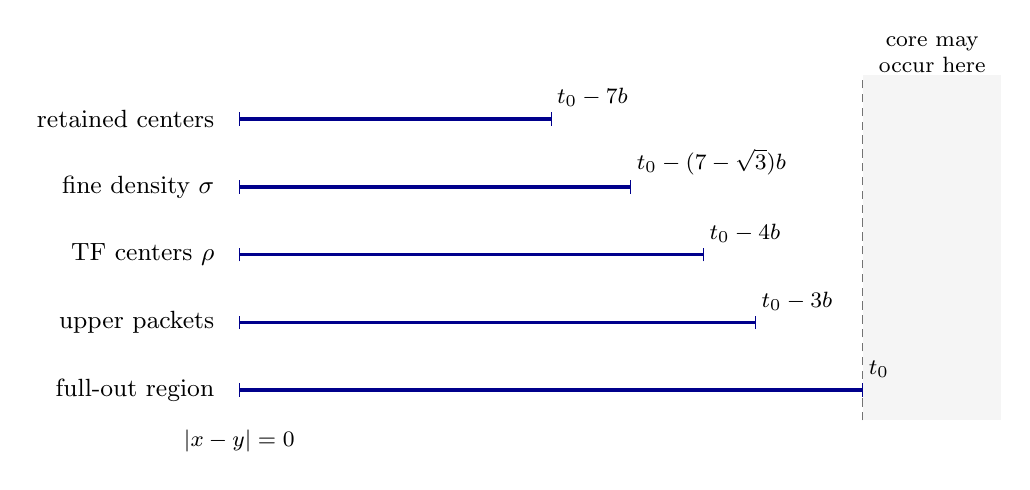
\begin{tikzpicture}[x=.88cm,y=.86cm,font=\small]
  \fill[black!4] (9,-.45) rectangle (11,4.65);
  \draw[densely dashed,black!55] (9,-.45)--(9,4.65);
  \node[align=center,font=\footnotesize] at (10,4.95) {core may\\occur here};
  \foreach \yy/\endx/\lefttext/\righttext in {
       4/4.5/{retained centers}/{$t_0-7b$},
       3/5.65/{fine density $\sigma$}/{$t_0-(7-\sqrt3)b$},
       2/6.7/{TF centers $\rho$}/{$t_0-4b$},
       1/7.45/{upper packets}/{$t_0-3b$},
       0/9/{full-out region}/{$t_0$}} {
    \node[anchor=east] at (-.22,\yy) {\lefttext};
    \draw[very thick,blue!55!black] (0,\yy)--(\endx,\yy);
    \draw[blue!55!black] (0,\yy-.1)--(0,\yy+.1);
    \draw[blue!55!black] (\endx,\yy-.1)--(\endx,\yy+.1);
    \node[anchor=south west,font=\footnotesize,inner sep=2pt]
      at (\endx,\yy+.09) {\righttext};
  }
  \node[anchor=north,font=\footnotesize] at (0,-.45) {$|x-y|=0$};
\end{tikzpicture}

 \caption{Radial supports in the interior comparison (schematic, not to
 scale). Fine smears of retained particles lie inside the TF domain,
 and the upper packets remain at distance at least $3b$ from the
 conditional core. This particle-support geometry is common to both
 applications. The atomic distance scale makes $B(y,20a)$ free of
 nuclei; the molecular scale may leave nuclei there, and their packet
 loss is retained in \eqref{m:eq:screen-comparison}.}
 \label{m:fig:screen-patch}
\end{figure}

\paragraph{Choice of cut and the conditional field.}
For a candidate $t\in[5a,6a]$, let the cut transition in a shell of
width $b$, using sine and cosine of an angle.  Let $n_{\rm del}$ count
the out particles not retained.  Such a particle lies in
$t-7b\le|x-y|\le t+b$.  For each raw pair of particles the set of
$t$ for which both lie in this shell has length at most $8b$.
Averaging over $t$ therefore bounds its expected squared count by
$C\beta Pm^2$, since $B(y,7a)$ has a bounded comparable-scale cover.
The same averaging, applied to the nuclear integral, uses
\eqref{m:eq:screen-nuclear-power} to give a bound $C\beta a^{-7}$.
Averaging the sum of the two normalized nonnegative quantities selects
one $t_0$ for which both bounds hold:
\begin{equation}\label{m:eq:screen-deleted-shell}
 \begin{gathered}
 \E n_{\rm del}^2\le C\beta Pm^2,\qquad
 \E n_o^2\le CPm^2,\qquad
 \mathrm{IMS}\le Cb^{-2}\sqrt Pm,\\
 \int_{\{t_0-7b\le|x-y|\le t_0+b\}}V_{\rm loc}^{5/2}
       \le C\beta a^{-7}.
 \end{gathered}
\end{equation}
The full out-count and IMS bounds in the same display follow from
the comparable-scale cover and $\E n_z\le\sqrt Pm_z$.

On the cut support and on $\Omega$ we have
\begin{equation}\label{m:eq:screen-field-cap}
 \Phi_X\le V_{\rm loc}+F,\qquad F\ge0,\qquad
 \|F\|_2\le C\frac{\sqrt Pm}{a}.
\end{equation}
To see this, the raw sources outside $B(y,20a)$ give a harmonic
conditional field on $B(y,10a)$; these electrons are all core particles.
Its value at $v\in B(y,10a)$ is at most
$\E[J_v\mid X]+Ca^{-4}$, by the same exclusion comparison as
\eqref{m:eq:screen-harmonic-raw}.  Take $F$ to be the positive supremum
on $B(y,7a)$.  Harmonic means and
Lemma~\ref{m:lem:screen-positive-field} prove \eqref{m:eq:screen-field-cap}.
The cells of this initial cut have scale comparable to $a$ and
$D_z\le C\beta^{-1}$, so \eqref{m:eq:screen-patch-condition} verifies
that lemma's hypothesis.

\paragraph{The unconstrained minimizer.}
The core is at distance at least $4b$ from $\Omega$, so its potential
is bounded and smooth there.  Hence $\Phi_X\in L^{5/2}(\Omega)$.
Young's inequality makes \eqref{m:eq:screen-tf-functional} coercive in
$L^{5/3}$.  The positive Coulomb form is weakly lower semicontinuous:
by Lemma~\ref{lem:loc-coulomb} it is a squared Hilbert norm, or
one may express it as the supremum of its affine dual forms.
The direct method on the closed positive cone gives a minimizer,
and strict convexity of the kinetic term gives uniqueness.
Nonnegative variations, followed by signed compact multiplicative
variations, give
\[
 \frac53\cT\rho^{2/3}-\Phi_X+K*\rho\ge0,
 \qquad
 \left(\frac53\cT\rho^{2/3}-\Phi_X+K*\rho\right)\rho=0,
\]
which is \eqref{m:eq:screen-tf-equation}.

This minimizer depends continuously in $L^{5/3}$ on its field in
$L^{5/2}$.  Indeed convergent fields give uniformly bounded minimizers;
weak lower semicontinuity and comparison with the limit minimizer
identify each weak limit and give convergence of the minimum values.
Lower semicontinuity of $D$ then forces convergence of the kinetic
norms.  Uniform convexity of $L^{5/3}$ gives strong convergence.
The conditional field, being jointly measurable and taking values
in the separable space $L^{5/2}(\Omega)$, is measurable as a
function with values in that space.  The continuity just proved
establishes the stated measurability of $\rho$.

The diameter of $\Omega$ is at most $12a$, so
$D(\rho)\ge(\int\rho)^2/(24a)$.  The minimum is nonpositive because
zero is admissible.  Absorbing $V_{\rm loc}$ with Young's inequality
in \eqref{m:eq:screen-field-cap} gives
\[
 \frac{(\int\rho)^2}{Ca}\le Ca^{-7}+F\int\rho.
\]
It follows that
\begin{equation}\label{m:eq:screen-tf-mass}
 \int\rho\le C(aF+a^{-3}),\qquad
 \int\rho^{5/3}\le C(aF^2+a^{-7}).
\end{equation}
When $V_{\rm loc}=0$, the same nonpositive-minimum argument uses
only $\Phi_X\le F$ and gives the sharper estimates
\begin{equation}\label{a:eq:screen-minimizer-mass}
 \int\rho\le CaF,\qquad \int\rho^{5/3}\le CaF^2.
\end{equation}
In particular all trial errors below are integrable in $X$.

\paragraph{Upper quantum comparison.}
The centers $\rho$ lie in $\Omega=B(y,t_0-4b)$; packets of width
$b$ remain at distance at least $3b$ from the core.  Thus
Lemma~\ref{lem:loc-hole-trial} applies, and radial smearing leaves
the core potential unchanged.  The nuclear loss is bounded at
centers by
\[
 V_b^{\rm loss}(x)=\sum_{R_m\in B(y,20a)}
             \frac{z_m}{|x-R_m|}\1_{\{|x-R_m|\le2b\}}.
\]
Weighted convexity, the total local charge bound, and integration of
$|x|^{-5/2}$ over a ball of radius $2b$ give
\[
 \int(V_b^{\rm loss})^{5/2}\le C\beta^{1/2}a^{-7}.
\]
Nuclei not in the indicated local ball are harmonic on all packets.
Young's inequality now gives, pathwise,
\begin{equation}\label{m:eq:screen-patch-upper}
 E\le e_X+\mathcal T_X(\rho)+Cb^{-2}\int\rho
       +C\epsilon\int\rho^{5/3}
       +C\epsilon^{-3/2}\beta^{1/2}a^{-7}.
\end{equation}

\paragraph{Lower quantum comparison.}
Reserve a fraction $\epsilon T_o$ of the out kinetic energy.  The
coarse kinetic inequality absorbs both $V_b^{\rm loss}$ and the
nuclear attraction of deleted particles, at cost
$C\epsilon^{-3/2}\beta^{1/2}a^{-7}$, using
\eqref{m:eq:screen-deleted-shell}.  The deleted $F$ contribution costs
at most
\[
 \|F\|_2\|n_{\rm del}\|_2\le C\sqrt\beta Pe.
\]
The retained fine density $\sigma$ is supported in $\Omega$, because
its centers have radius less than $t_0-7b$ and its kernel radius is
$\sqrt3b$.  The core potential is harmonic on these kernels, and
the loss of nuclear attraction is again covered by $V_b^{\rm loss}$
at the actual particle positions.  Applying the remaining fraction
of Lemma~\ref{lem:loc-cubes} and its pair-repulsion bound in the
localization identity gives
\begin{align}\label{m:eq:screen-patch-lower}
 q_n[\psi]+\mathrm{IMS}
 &\ge\E\left[e_X+\mathcal T_X(\sigma)
                    -\epsilon\cT\int\sigma^{5/3}\right]
       -C\mathcal R,\\
 \mathcal R&=\epsilon^{-3/2}\beta^{1/2}a^{-7}
             +\sqrt\beta Pe+b^{-1}\sqrt Pm
             +b^{-2}\left(P^{2/3}m^{4/3}+\sqrt Pm\right).\notag
\end{align}
Here $\E n_o^{4/3}\le(\E n_o^2)^{2/3}$; no higher out-count
moment is required.

The Euler equation gives the exact expansion
\begin{equation}\label{m:eq:screen-tf-expansion}
 \mathcal T_X(\sigma)-\mathcal T_X(\rho)
       =D(\sigma-\rho)+\mathcal L+\int W_-\sigma.
\end{equation}
Besides being nonnegative, the convex remainder satisfies
\[
 \mathcal L\ge c\int\sigma^{5/3}-C\int\rho^{5/3},
\]
by Young's inequality applied to the tangent term.  For small
$\epsilon$ this absorbs $\epsilon\cT\int\sigma^{5/3}$ into half
of $\mathcal L$, with error $C\epsilon\int\rho^{5/3}$.
Average \eqref{m:eq:screen-patch-upper}, compare it with
\eqref{m:eq:screen-patch-lower}, and use
\eqref{m:eq:screen-tf-mass}, \eqref{m:eq:screen-field-cap}, and the IMS
bound.  The terms $\epsilon\E\int\rho^{5/3}$ cost $C\epsilon Pe$;
the packet kinetic term costs
$Cb^{-2}(\sqrt Pm+a^{-3})\le Cb^{-2}\sqrt Pm$.
This proves \eqref{m:eq:screen-comparison}, after multiplying its
constant to restore the full nonnegative remainder, and also the
asserted bound for $\E\int\sigma^{5/3}$.

\paragraph{The source-free improvement.}
If $\nu(B(y,20a))=0$, every nucleus and the conditional core are
outside the packet supports.  The field $\Phi_X$ is harmonic on
those supports, so radial averaging is exact and the upper comparison
is
\begin{equation}\label{a:eq:screen-upper}
 E\le e_X+\mathcal T_X(\rho)+Cb^{-2}\int\rho.
\end{equation}
For the lower comparison, use all the out kinetic energy.
Harmonicity and the deleted-count bound give
\[
 \sum_{i\ \mathrm{retained}}\Phi_X(x_i)=\int\Phi_X\sigma,
 \qquad \E(Fn_{\rm del})\le C\sqrt\beta Pe.
\]
The full sharp kinetic
and pair bounds of Lemma~\ref{lem:loc-cubes} therefore give
\begin{equation}\label{a:eq:screen-lower}
 q_n[\psi]+\mathrm{IMS}
 \ge\E[e_X+\mathcal T_X(\sigma)]
 -C\left[\sqrt\beta Pe+b^{-1}\sqrt Pm
       +b^{-2}(P^{2/3}m^{4/3}+\sqrt Pm)\right].
\end{equation}
Subtract the average upper inequality and use the exact expansion
\eqref{m:eq:screen-tf-expansion}, the mass estimate
\eqref{a:eq:screen-minimizer-mass}, and the IMS bound.  This proves
\eqref{a:eq:screen-patch}, including its full convex remainder,
without the nuclear loss or an $\epsilon$ error.

There is a useful separate kinetic bound.  In the localization identity
use only $e_X\ge E$, drop pair repulsion, and use
\eqref{m:eq:screen-field-cap}.  Half the coarse kinetic inequality
absorbs $V_{\rm loc}$ at cost $Ca^{-7}$; also
$\E(Fn_o)\le CPe$.  The result is
\eqref{m:eq:screen-out-kinetic}.

\paragraph{Interior field bound.}
The core vanishes in $B(y,4a)$ and this ball lies in $\Omega$.
There
\[
 \Delta W=-4\pi\nu+\cF W_+^{3/2}.
\]
Put $s=4a$ and
\[
 U(x)=V_{\rm loc}(x)+\frac{C s^4}{(s^2-|x-y|^2)^4}.
\]
The Laplacian of the bump is at most
$80Cs^6/(s^2-|x-y|^2)^6$.  For a sufficiently large universal $C$
this is at most $\cF$ times its $3/2$ power.  Thus $U$ is a
supersolution for the displayed equation.  The difference $W-V_{\rm loc}$
is bounded above: the far nuclear field is bounded on this ball,
the core potential is nonnegative, and $K*\rho\ge0$.
Consequently $(W-U)_+$ has compact support inside the ball.
Nuclear singularities cancel in $W-U$, which is locally $H^1$;
testing the difference inequality by its positive part yields
\[
 -\int|\nabla(W-U)_+|^2
 \ge\cF\int_{\{W>U\}}(W_+^{3/2}-U^{3/2})(W-U)\ge0.
\]
The test is valid by compact $H^1$ approximation: the densities
are locally in $L^{5/3}$, and the nuclear point terms have already
canceled.  Hence $W\le U$.  On $B(y,3a)$ the bump is $Ca^{-4}$,
proving the first part of \eqref{m:eq:screen-interior-upper}.
If $V_{\rm loc}=0$, this yields $W\le Ca^{-4}$; the Euler equation
then gives $\rho\le Ca^{-6}$ and proves
\eqref{a:eq:screen-interior}.  In this source-free case,
\begin{equation}\label{a:eq:screen-poisson}
 \Delta W=\cF W_+^{3/2}=4\pi\rho
       \quad\hbox{on }B(y,4a).
\end{equation}
Finally, weighted powers and $\nu(B(y,20a))\le a^{-3}$ give
\[
 \int_{B(y,2a)}\rho
 \le C\int_{B(y,2a)}(V_{\rm loc}^{3/2}+a^{-6})
 \le C(a^{-9/2}a^{3/2}+a^{-3})\le Ca^{-3}.
\]
\end{proof}

\subsection{Closing the count estimate}

The comparison in a hole bounds its electron count through a smooth
Coulomb test.  The resulting inequality improves any sufficiently
large value of the provisional constant $P$, and therefore makes
that constant universal.

\begin{lemma}[Local second moments]\label{m:lem:screen-count}
For every normalized $\delta$-state in any finite sector and every
$y\in\mathcal Y$,
\begin{equation}\label{m:eq:screen-count}
 \E n_y^2\le C\left(\max(a_y^{-6},1)+\delta a_y\right).
\end{equation}
In particular the number $P$ in
\eqref{m:eq:screen-count-normalization} is at most a universal constant.
\end{lemma}

\begin{proof}
Fix small $\epsilon>0$ and $0<\beta<1/100$, to be chosen in that
order.  We need only consider $P\ge\beta^{-4}$, since $\beta$ will
be fixed universally.  Then $\beta^{-2}/(am)\le\sqrt P$ at every
target, and the patch of Lemma~\ref{m:lem:screen-patch} is available.
Every raw particle in $B_y$ is retained, and its fine smear is
contained in $B(y,1.1a)$ because $\beta<1/100$.
Choose a nonnegative smooth $\chi$, equal to one there, supported
in $B(y,2a)$, with $\|\nabla\chi\|_2\le C\sqrt a$.
Lemma~\ref{lem:loc-coulomb} and
\eqref{m:eq:screen-interior-upper} give
\[
 n_y\le\int\chi\sigma
 \le Ca^{-3}+C\sqrt{aD(\sigma-\rho)},\qquad
 \E n_y^2\le Ca^{-6}+Ca\,\E D(\sigma-\rho).
\]
Divide by $Pm^2$ and use \eqref{m:eq:screen-comparison}.  Since
$\delta a\le m^2$, the result is at most
\begin{align}\label{m:eq:screen-bootstrap-ratio}
 C\bigg[&P^{-1}+\epsilon+\sqrt\beta
       +\frac{\epsilon^{-3/2}\beta^{1/2}}P
       +\frac{\beta^{-1}}{\sqrt Pm}\\
       &+\frac{\beta^{-2}}{P^{1/3}am^{2/3}}
       +\frac{\beta^{-2}}{\sqrt Pam}\bigg].\notag
\end{align}
In the atomic distance geometry, using \eqref{a:eq:screen-patch}
instead gives the sharper intermediate inequality
\begin{equation}\label{a:eq:screen-count-bootstrap}
 \frac{\E n_y^2}{Pm_y^2}
 \le C\left[P^{-1}+\sqrt\beta
 +\frac{\beta^{-1}}{\sqrt Pm_y}
 +\frac{\beta^{-2}}{P^{1/3}a_ym_y^{2/3}}
 +\frac{\beta^{-2}}{\sqrt P a_ym_y}\right].
\end{equation}
For the common bound it suffices to use
\eqref{m:eq:screen-bootstrap-ratio} in both geometries.
First choose $\epsilon$ small, then $\beta$ small, and finally a
universal threshold $P_0$ large.  The inequalities
\eqref{m:eq:screen-normalization-inequalities} show that the expression
is at most $1/2$ whenever $P>P_0$.  Enlarge $P_0$ so that
$P_0\ge\beta^{-4}$; this verifies
\eqref{m:eq:screen-patch-condition} at every target.  If $P>P_0$, we
would obtain $\E n_y^2/m_y^2\le P/2$ for every $y$, contradicting
the definition of $P$.  Thus $P\le P_0$.  Since
$m_y^2\le2\max(a_y^{-6},1)+2\delta a_y$, this proves
\eqref{m:eq:screen-count}.
\end{proof}

\begin{proposition}[Uniform local counts and conditional fields]
\label{a:prop:screen-local}
In either geometry, every normalized $\delta$-state in a finite sector
satisfies $P\le C$.  Fix $y\in\mathcal Y$.  Suppose the initial
finite sequence of cuts has total out support covered by at most
$C_0$ cells $B_z$, with $C_0^{-1}\le a_z/a_y\le C_0$, and satisfies
the gradient hypothesis of Lemma~\ref{m:lem:screen-positive-field}.
The absent-cut case is allowed.  Then
\begin{equation}\label{a:eq:screen-local}
 P\le C,\qquad
 \big\|(\E[J_y\mid X])_+\big\|_2
             \le C(C_0)\frac{m_y}{a_y}.
\end{equation}
Neither constant depends on the nuclear system, particle number,
state, target, or $\delta$.
\end{proposition}

\begin{proof}
The count assertion is Lemma~\ref{m:lem:screen-count}.
Comparable scales have comparable $m$ and $e=m^2/a$, uniformly in
$\delta$, so $e_*\le C(C_0)e_y$ in
Lemma~\ref{m:lem:screen-positive-field}.  Substitute $P\le C$
into that lemma to obtain the field assertion.
\end{proof}

\begin{lemma}[Fine comparison and local density]\label{m:lem:screen-density}\label{a:cor:screen-refined}
There is a universal $a_0>0$ with the following property.  If
$a=a_y<a_0$ and $\psi$ is a $\delta$-state with
$\delta\le a^{-7+0.02}$, choose the patch of
Lemma~\ref{m:lem:screen-patch} with $b=a^{1+0.2}$.  Its densities obey
\begin{equation}\label{m:eq:screen-fine-error}
 \E\left[D(\sigma-\rho)+\mathcal L+\int W_-\sigma\right]
       \le Ca^{-7+0.02},\qquad
 \E\int\sigma^{5/3}\le Ca^{-7}.
\end{equation}
The raw one-body density satisfies
\begin{equation}\label{m:eq:screen-density}
 \int_{B(y,4a)}\rho_\psi^{5/3}\le Ca^{-7}.
\end{equation}
In particular, the two estimates needed in the atomic application are
\begin{equation}\label{a:eq:screen-refined}
 \E\left[D(\sigma-\rho)+\int W_-\sigma\right]\le Ca^{-7+.02},
 \qquad \int_{B(y,4a)}\rho_\psi^{5/3}\le Ca^{-7}.
\end{equation}
\end{lemma}

\begin{proof}
Take $\beta=a^{0.2}$ and $\epsilon=a^{0.02}$.  The energy assumption
gives $m\le Ca^{-3}$, while
$\beta^{-2}/(am)\le a^{1.6}$, so the patch hypothesis holds for
small $a$.  By Lemma~\ref{m:lem:screen-count}, $P\le C$.
The terms on the right of \eqref{m:eq:screen-comparison} are bounded
respectively by constant multiples of
\[
 a^{-6.98},\quad a^{-6.98}+a^{-6.9},\quad
 a^{-6.93},\quad a^{-4.2},\quad a^{-6.4}+a^{-5.4}.
\]
All are at most $Ca^{-7+0.02}$ for $a<1$, proving
\eqref{m:eq:screen-fine-error}.  Equation~\eqref{m:eq:screen-out-kinetic}
gives $T_o\le Ca^{-7}$.  Since the cut is full out on $B(y,4a)$,
the out density equals $\rho_\psi$ there.  Applying
Lemma~\ref{lem:loc-kinetic} proves \eqref{m:eq:screen-density}.
\end{proof}

\begin{corollary}[Raw near-Coulomb bound]
Under the hypotheses of Lemma~\ref{m:lem:screen-density}, for
$0<u\le4a$,
\begin{equation}\label{a:eq:screen-near-coulomb}
 \E\sum_{|x_i-y|<u}\frac1{|x_i-y|}
       \le Ca^{-4}(u/a)^{1/5}.
\end{equation}
\end{corollary}

\begin{proof}
The expectation is $\int_{B(y,u)}|x-y|^{-1}\rho_\psi(x)\,dx$.
H\"older's inequality, the raw density bound, and direct radial
integration give
\[
 \int_{B(y,u)}\frac{\rho_\psi(x)}{|x-y|}\,dx
 \le\left(\int_{B(y,4a)}\rho_\psi^{5/3}\right)^{3/5}
       \left(\int_{|z|<u}|z|^{-5/2}\,dz\right)^{2/5}
 \le Ca^{-21/5}u^{1/5}.
\]
This is the stated bound in either geometry.
\end{proof}

\subsection{Source-free oscillation and atomic annuli}

The next estimate controls also a very negative field.  It applies
when the patch contains no local nuclear source; molecular patches
containing nuclei instead use the offset oscillation estimate proved
with the nuclear splitting below.

\begin{lemma}[Interior oscillation]
\label{a:lem:screen-oscillation}
For every patch in Lemma~\ref{a:lem:screen-patch} with
$\nu(B(y,20a))=0$, and every
$0<s'\le a/2$, almost surely in its data,
\begin{equation}\label{a:eq:screen-oscillation}
 \sup_{x\in B(y,s')}|W(x)-W(y)|
       \le C\frac{s'}a\bigl(a^{-4}+W(y)_-\bigr).
\end{equation}
\end{lemma}

\begin{proof}
By \eqref{a:eq:screen-poisson} and \eqref{a:eq:screen-interior},
$0\le\Delta W\le Ca^{-6}$ on $B(y,2a)$.  Write
\[
 Q(x)=\frac1{4\pi}
       \int_{B(y,2a)}\frac{\Delta W(z)}{|x-z|}\,\dd z.
\]
For $x\in B(y,2a)$, direct integration of $|x-z|^{-1}$ and
$|x-z|^{-2}$ gives
\[
 0\le Q(x)\le Ca^{-4},\qquad |\nabla Q(x)|\le Ca^{-5}.
\]
Since $\Delta Q=-\Delta W$ inside that ball,
$H=W+Q$ is harmonic there.  By \eqref{a:eq:screen-interior},
$H\le C_1a^{-4}$.  Choose $C_2>C_1$ universally and put
$h=C_2a^{-4}-H$, a positive harmonic function on $B(y,2a)$.
The Poisson formula on a sphere of radius $3a/2$ gives
\[
 \sup_{B(y,a)}|\nabla h|\le Ca^{-1}h(y).
\]
Indeed the differentiated Poisson kernel on $B(y,a)$ is bounded
by $C/a$ times its value at the center; integrating the
nonnegative boundary values gives precisely this inequality.
Also $h(y)\le Ca^{-4}+W(y)_-$, since $Q(y)\ge0$.
Integrate the gradient along segments in $B(y,s')$, and add
the bound for $\nabla Q$.  This proves
\eqref{a:eq:screen-oscillation}.
\end{proof}

\begin{corollary}[Annular counts]
\label{a:cor:screen-annular}
In the atomic distance geometry, for every
$0<\lambda<\Lambda<\infty$ and $u>0$, every normalized
$\delta$-state of finite particle number satisfies
\begin{equation}\label{a:eq:screen-annular}
 \left\|\#\{i:\lambda u<|x_i|<\Lambda u\}\right\|_2
 \le C_{\lambda,\Lambda}
       \bigl(\max(u^{-3},1)+\sqrt{\delta u}\bigr).
\end{equation}
All constants are independent of $Z$ and of the particle number.
\end{corollary}

\begin{proof}
The compact annulus $\{\lambda\le|x|\le\Lambda\}$ has a finite
cover by cells $B_z$ whose radii are comparable to one, with
constants allowed to depend on $\lambda,\Lambda,L$.  Dilate this
cover by $u$.  Because $a_{uz}=ua_z$, the dilated balls are
again cells, now with radii comparable to $u$.  The annular count
is bounded by their sum of counts.  Minkowski's inequality and
\eqref{a:eq:screen-local} bound its $L^2$ norm by $C\sum_z m_z$,
which is the right side of \eqref{a:eq:screen-annular}.  Boundary
spheres carry zero raw probability, since the one-electron
density is absolutely continuous.  Thus the same estimate holds
with any choice of open or closed endpoints.
\end{proof}

\section{Common observation and change-of-law estimates}\label{sec:observations}

The two geometries use different master widths and nuclear fields, but
share the observation likelihood, the cost of imposing an event, and
the transfer from the observed field to a fresh patch field. We prove
these statements here. In particular, the last transfer compares
expectations under a specified law; it does not identify the two
conditional fields on individual configurations.

\subsection{Likelihoods and conditional versions}

Let $\Psi$ be a normalized antisymmetric state in a finite $n$-electron
sector. Under a probability law $P$, raw positions and spins
$(x,\boldsymbol\sigma)$ have density $|\Psi|^2$. Fix finitely many
widths $\ell_0,\ldots,\ell_{m-1}>0$. Independently of the raw data,
take independent scalar noises $U_{ji,b}$ with density
\[
 \zeta(u)=c_\zeta\exp\!\left(-\frac1{1-u^2}\right)
                         \1_{(-1,1)}(u).
\]
At scale $j$, form the labeled observations
$\widehat Y_{ji,b}=x_{i,b}+\ell_jU_{ji,b}$ and then forget the
particle labels separately in each array. Represent the result by
its lexicographically sorted tuple $Y_j$ in the strict sorted chamber
$\mathcal C\subset(\R^3)^n$. Ties have probability zero. Set
\[
 \mathcal F_j=\sigma(Y_j,\ldots,Y_{m-1}),\qquad
 \mathcal F_m=\{\varnothing,\Omega\}.
\]
Thus the sigma-fields decrease as $j$ increases.

Let $t_z$ be a deterministic measurable width with
$t_z\ge t_{\min}>0$ for the fixed system, and use the smooth radial
packet of Section~\ref{sec:localization} to define
$\mathcal K_z(y)=g_{t_z}(y-z)^2$. Write
$V=V_s+V_c$, where $V_s$ is the deterministic nuclear potential
retained in the observed field. In the molecular application it is
the smoothed nuclear potential. In the atomic application
$V_s=V$ and $V_c=0$. Where relevant put
$\nu_s=-(4\pi)^{-1}\Delta V_s$ distributionally; it is the
smoothed nuclear measure in the first case and the original
point measure in the second.

\begin{lemma}[Conditional densities and fields]\label{lem:obs-data}
There are jointly Borel versions of
\[
 \mu_j(y)=\E_P\!\left[\sum_{i=1}^n\mathcal K_{x_i}(y)
                                      \mid\mathcal F_j\right],
 \qquad H_j(y)=V_s(y)-(K*\mu_j)(y),
\]
with the following properties. At every positive-density data tuple,
$\mu_j\ge0$, $\int\mu_j=n$, and $\mu_j$ is smooth in its spatial
variable. Every spatial derivative has a deterministic bound for
the fixed system. The potential $K*\mu_j$ is $C^1$, with bounded
value and gradient, and
\begin{equation}\label{eq:obs-poisson}
 \Delta H_j=-4\pi\nu_s+4\pi\mu_j
\end{equation}
in distributions. In particular, the always valid regularity
statement is that $H_j-V_s$ is $C^1$ and bounded with bounded
gradient. If $V_s$ and its gradient are bounded and continuous,
these conclusions hold for $H_j$ itself. Conditional averaging
satisfies
\begin{equation}\label{eq:obs-tower}
 \E_P[\mu_j(y)\mid\mathcal F_{j+1}]=\mu_{j+1}(y),\qquad
 \E_P[H_j(y)\mid\mathcal F_{j+1}]=H_{j+1}(y)
\end{equation}
where $V_s(y)$ is finite. The same towers hold for nonnegative
spatial integrals, and for integrable signed observables.
These statements include the trivial data at $j=m$. None of the
fixed-system regularity bounds is asserted to be uniform in the
nuclear system or in $t_{\min}$.
\end{lemma}

\begin{proof}
On $\mathcal C$ the exact likelihood of an array is
\begin{equation}\label{eq:obs-likelihood}
 L_j(x,Y_j)=\sum_{\pi\in S_n}\prod_{i=1}^n\prod_{b=1}^3
 \ell_j^{-1}\zeta\!\left(
           \frac{Y_{j,\pi(i),b}-x_{i,b}}{\ell_j}\right).
\end{equation}
Set it equal to zero outside the chamber. Integration of the
permutation sum over $\mathcal C$ equals integration of the labeled
product over all arrays, and is therefore one. Define
\[
 \Lambda_{\ge j}(x,Y)=\prod_{h=j}^{m-1}L_h(x,Y_h),\qquad
 p_{\ge j}(Y)=\sum_{\boldsymbol\sigma}\int
       |\Psi(x,\boldsymbol\sigma)|^2\Lambda_{\ge j}(x,Y)\dd x,
\]
with the empty product and $p_{\ge m}$ both equal to one. At a tuple
with $p_{\ge j}>0$, use the probability density
$|\Psi|^2\Lambda_{\ge j}/p_{\ge j}$ as the conditional raw law.
Equivalently, the conditional mean of a nonnegative Borel raw
observable $G$ is the ratio
\[
 \frac{\displaystyle\sum_{\boldsymbol\sigma}\int
       G(x,\boldsymbol\sigma)|\Psi(x,\boldsymbol\sigma)|^2
                      \Lambda_{\ge j}(x,Y)\dd x}
      {p_{\ge j}(Y)}.
\]
On zero-density tuples use the unconditional raw law. All these
versions are jointly Borel, including their dependence on an
additional spatial variable. At every parent tuple with
$p_{\ge j+1}>0$, the conditional density of the next array is
$p_{\ge j}/p_{\ge j+1}$. Tonelli's theorem and $\int L_j\dd Y_j=1$
show that it integrates to one. Substitution of the ratios gives
the tower property, also after nonnegative spatial integration;
positive and negative parts give the integrable signed case.

For each multi-index $\alpha$,
$|\partial_y^\alpha\mathcal K_z(y)|
 \le C_\alpha t_{\min}^{-3-|\alpha|}$ uniformly in $z,y$.
Differentiation under the conditional integral therefore gives all
claimed derivatives and bounds. Tonelli gives the mass $n$.
For the potential and its gradient, split the kernels $|u|^{-1}$
and $|u|^{-2}$ at unit distance. The near parts are integrable and
are controlled by $\|\mu_j\|_\infty$; the far parts are controlled
by $n$. Splitting again at a small radius, then using dominated
convergence on its complement, proves continuity of the potential
and gradient. Finally $-\Delta K=4\pi\delta_0$ gives
\eqref{eq:obs-poisson}. In the atomic case this argument does not
remove the nuclear singularity of $V_s$.
\end{proof}

\subsection{Dimension-free energy cost}

\begin{lemma}[Energy cost of a data event]\label{lem:obs-tilt}
Suppose $\Psi$ is an eigenstate of its sector Hamiltonian with
energy $e_\Psi$, where $0\le e_\Psi-E\le D_0$. In particular,
$e_\Psi=E_n$ for a sector ground state. Suppose further that
\[
 \sum_{h=j}^{m-1}\ell_h^{-2}\le C_\ell\ell_j^{-2}
\]
with a fixed numerical $C_\ell$. This holds for the dyadic scales
$\ell_h=r_h^{1.01}$, $r_{h+1}=2r_h$, with
$C_\ell=(1-2^{-2.02})^{-1}$. If $A\in\mathcal F_j$ has probability
$p=P(A)>0$, put $p_A(x)=P(A\mid x)$ and
\[
 \Psi_A=\sqrt{p_A(x)/p}\,\Psi.
\]
Then $\Psi_A$ is a normalized antisymmetric form-domain vector,
its raw position-and-spin law is the raw marginal of $P$ conditioned
on $A$, and
\begin{equation}\label{eq:obs-tilt}
 q_n[\Psi_A]\le e_\Psi+C\ell_j^{-2}\log^5(e/p)
       \le E+D_0+C\ell_j^{-2}\log^5(e/p).
\end{equation}
The constant depends only on $C_\ell$ and the chosen noise law,
not on $n$, the number of arrays, or the nuclear system. The same
assertion holds for an event of one unordered observation at any
width $\ell$, using $\ell$ in place of $\ell_j$. No upper bound
on the particle number in terms of the nuclear charge is needed.
\end{lemma}

\begin{proof}
In labeled observation coordinates place the sorting map inside
the indicator of $A$. The translated product density is continuously
differentiable in $L^1$, since $\zeta$ is smooth and compactly
supported. Hence $p_A$ is continuously differentiable even for a
Borel event. The scalar translation score is
\[
 S(u)=-\frac{\zeta'(u)}{\zeta(u)}
       =\frac{2u}{(1-u^2)^2},\qquad |u|<1.
\]
Its law is symmetric and centered. It satisfies
$\|S(U)\|_q\le Cq^2$ for $q\ge2$: indeed,
$T=(1-U^2)^{-1}$ has a finite exponential moment of every order
less than one, so integration of its exponential tail gives
$\|T\|_q\le Cq$, while $|S(U)|\le2T^2$.

For a unit vector $v\in\R^{3n}$ the directional derivative of the
likelihood pairs the event indicator with
\[
 Q_v=\sum_{h=j}^{m-1}\sum_{i=1}^n\sum_{b=1}^3
                    \ell_h^{-1}v_{i,b}S(U_{hi,b}).
\]
Multiplication by independent random signs preserves the joint law
of the independent symmetric scores. For deterministic coefficients,
\[
 \prod_\alpha\cosh(sc_\alpha)
       \le\exp\!\left(\frac{s^2}{2}\sum_\alpha c_\alpha^2\right)
\]
gives the Gaussian tail estimate and consequently
$\|\sum_\alpha\epsilon_\alpha c_\alpha\|_q
 \le C\sqrt q(\sum_\alpha c_\alpha^2)^{1/2}$.
Conditioning on the scores and then using the triangle inequality
in $L^{q/2}$ yields
\[
 \|Q_v\|_q\le Cq^{5/2}
       \left(\sum_{h,i,b}\ell_h^{-2}v_{i,b}^2\right)^{1/2}
       \le Cq^{5/2}\ell_j^{-1}.
\]
The identity $\sum_{i,b}v_{i,b}^2=1$ and the geometric square-sum
bound are precisely what avoid factors depending on dimension
or on the number of observations.

H\"older's inequality at fixed $x$ gives
$|D_vp_A(x)|\le Cq^{5/2}\ell_j^{-1}p_A(x)^{1-1/q}$.
For $p_A(x)>0$ choose $q=\max\{2,\log(e/p_A(x))\}$ and then take
the supremum over unit vectors. At a zero the gradient of the
nonnegative differentiable function $p_A$ vanishes. Therefore
\begin{equation}\label{eq:obs-score-gradient}
 |\nabla p_A|\le C\ell_j^{-1}p_A\log^{5/2}(e/p_A),
\end{equation}
with right side zero at $p_A=0$.

Regularize the square root by $\sqrt{p_A+\eta}$. Since
$\sqrt u\log^{5/2}(e/u)$ is bounded on $[0,1]$, these functions
have a common Lipschitz bound. Their uniform limit $\sqrt{p_A}$ is
Lipschitz. Its gradient vanishes almost everywhere on its zero set,
and the ordinary chain rule applies elsewhere. Thus
\[
 \left|\nabla\sqrt{p_A/p}\right|^2
       \le C\ell_j^{-2}\frac{p_A}{p}\log^5(e/p_A).
\]
The permutation sum in \eqref{eq:obs-likelihood} shows that $p_A$
is invariant under raw particle permutations and is spin independent.
The bounded Lipschitz multiplier therefore preserves antisymmetry
and the form domain. Its squared norm and its raw law are as claimed
by the definition of $p_A$.

Lemma~\ref{lem:sector-multiplier}, applied with eigenvalue $e_\Psi$,
now gives
\[
 q_n[\Psi_A]-e_\Psi
    \le C\ell_j^{-2}\E_P[\log^5(e/p_A(x))\mid A].
\]
Under this conditional law,
\[
 P\{p_A(x)<e^{-u}\mid A\}
   =p^{-1}\E_P[p_A\1_{\{p_A<e^{-u}\}}]
   \le\min\{1,e^{-u}/p\}\qquad(u\ge0).
\]
Integration of this tail, split at $\log(e/p)$, bounds the fifth
moment by $C\log^5(e/p)$ and proves \eqref{eq:obs-tilt}.
The proof for a single array is identical with the square-sum
constant equal to one.
\end{proof}

\subsection{Transfer to a fresh patch}

The following quantitative formulation isolates exactly the local
screening estimates needed by both applications. It allows either
a patch containing singular nuclei or a patch containing none.
The fine density below is the actual sum of packets around retained
raw particles, not its conditional average.

\begin{lemma}[Averaged field transfer]\label{lem:obs-transfer}
Fix a point $y$ where $V_s(y)$ is finite and a length $a>0$.
Let $A\in\mathcal F_j$ have positive $P$-probability, and let $Q$
be $P$ conditioned on $A$, extended by fresh localization labels.
Its raw marginal is the law of $\Psi_A$ from
Lemma~\ref{lem:obs-tilt}. Let $X$ denote the fresh patch data,
and let $\rho_X^c$ be the conditional density of core particles
under this tilted localization law. Partition the remaining raw
particles into retained and deleted particles. Let
\[
 \sigma=\sum_{i\ {\rm retained}}\vartheta_b(\cdot-x_i),\qquad
 h_X=V_s-K*\rho_X^c-K*\rho_X,\qquad W_X=V_c+h_X,
\]
where $\vartheta_b$ is the radial probability kernel of
Lemma~\ref{lem:loc-cubes}, supported in $B(0,\sqrt3b)$, and
$\rho_X\ge0$ is a measurably chosen patch comparison density.
Assume $\rho_X$ and
$\sigma$ belong to $L^{5/3}$ and have compact support for almost
every patch datum. Put $t=t_y$, $\tau=t/a$, and $\beta=b/a$,
and suppose $0<t,b\le a/10$. Assume the following estimates, with
fixed constants:
\begin{enumerate}
\item The master width $z\mapsto t_z$ is Lipschitz with constant
at most $1/2$. The raw one-particle density $\rho_{\Psi_A}$ satisfies
\[
 \int_{B(y,4a)}\rho_{\Psi_A}^{5/3}\le Ca^{-7}.
\]
\item Deleted particles have $|x_i-y|\ge ca$, and their count obeys
$\E_Q n_{\rm del}\le Ca^{-3}\sqrt\beta$.
\item For some $\varepsilon_a\ge0$,
\[
 \E_Q D(\rho_X-\sigma)\le Ca^{-7}\varepsilon_a^2.
\]
\item On $B(y,t)$ either the source-free bound
$\rho_X\le Ca^{-6}$ holds, or
\[
 \rho_X=k(W_X)_+^{3/2},\qquad
 W_X\le V_{\rm loc}+Ca^{-4},\qquad
 V_{\rm loc}(z)=\sum_\alpha\frac{q_\alpha}{|z-R_\alpha|},
 \qquad\sum_\alpha q_\alpha\le Ca^{-3},
\]
with $q_\alpha\ge0$. The latter alternative permits arbitrary
locations of the local nuclei.
\end{enumerate}
Then the two expectation towers are
\begin{equation}\label{eq:obs-two-towers}
 \E_Q(K*\mu_j)(y)=\E_Q P^{\rm ms}(y),\qquad
 \E_Q(K*\rho_X^c)(y)=\E_Q P^c(y),
\end{equation}
where $P^{\rm ms}$ is the potential of the raw master packets and
$P^c$ is the raw core potential. Moreover,
\begin{equation}\label{eq:obs-transfer}
 \begin{split}
 |\E_Q(H_j-h_X)(y)|\le Ca^{-4}\big[&
    \tau^{1/5}+\beta^{1/5}+\sqrt\beta
      +\varepsilon_a\tau^{-1/2}\\
    &+R(\tau)+(\tau+\sqrt3\beta)^{1/5}\big],
 \end{split}
\end{equation}
where $R(\tau)=\tau^2$ in the source-free alternative and
$R(\tau)=\tau^2+\tau^{1/2}$ in the nuclear alternative.
Thus the common upper bound $R(\tau)\le C\tau^{1/2}$ is always
available. All constants are independent of the number of particles;
they depend only on the constants in the displayed hypotheses.
\end{lemma}

\begin{proof}
Write
\[
 P^{\rm raw}(y)=\sum_iK(y-x_i),\qquad
 P^{\rm ms}(y)=\sum_i(K*\mathcal K_{x_i})(y),\qquad
 P^{\rm raw}=P^c+P^{\rm ret}+P^{\rm del}.
\]
The first identity in \eqref{eq:obs-two-towers} follows by multiplying
the original $P$-conditional expectation defining $\mu_j$ by
$\1_A$, using $A\in\mathcal F_j$, and dividing by $P(A)$.
The fresh labels do not alter this expectation. For the second
identity, condition the raw-plus-label marginal of $Q$ on $X$.
That marginal is exactly the localization law of $\Psi_A$; the
original observations can be integrated out. Tonelli justifies
both identities initially for nonnegative potentials. In
particular the first tower is under the original observation
law, while the second uses the fresh tilted patch law.

Subtracting the definitions of $H_j$ and $h_X$, and then using
these towers, gives the exact algebraic identity
\begin{equation}\label{eq:obs-transfer-decomposition}
 \begin{split}
 \E_Q(H_j-h_X)(y)=\E_Q\big[&
 (P^{\rm raw}-P^{\rm ms})-P^{\rm del}\\
 &-(P^{\rm ret}-K*\sigma)+K*(\rho_X-\sigma)\big](y).
 \end{split}
\end{equation}
The estimates below also establish finiteness of all terms, so this
subtraction involves no difference of infinite expectations.

For $0<u\le4a$, the local density bound and H\"older's inequality
give
\begin{equation}\label{eq:obs-near-coulomb}
 \begin{split}
 \E_Q\sum_{|x_i-y|<u}K(y-x_i)
 &\le\left(\int_{B(y,4a)}\rho_{\Psi_A}^{5/3}\right)^{3/5}
       \left(\int_{|z|<u}|z|^{-5/2}\dd z\right)^{2/5}\\
 &\le Ca^{-4}(u/a)^{1/5}.
 \end{split}
\end{equation}
The complementary raw potential is bounded by $n/(4a)$.
By radial smearing, $P^{\rm raw}-P^{\rm ms}\ge0$ and only centers
with $|x_i-y|\le t_{x_i}$ can contribute. Lipschitz continuity of
the width implies $|x_i-y|\le t_y+|x_i-y|/2$, hence these centers
lie in $B(y,2t)$. Equation~\eqref{eq:obs-near-coulomb} bounds its
mean by $Ca^{-4}\tau^{1/5}$. The same Newton comparison for each
fine packet gives
\[
 0\le\E_Q(P^{\rm ret}-K*\sigma)(y)
             \le Ca^{-4}\beta^{1/5}.
\]
The distance and count assumptions for the deleted particles give
$\E_Q P^{\rm del}(y)\le Ca^{-4}\sqrt\beta$.

For the signed density difference take
$v_t(z)=\min\{|y-z|^{-1},t^{-1}\}$. This is in $\dot H^1$ and
\[
 \|\nabla v_t\|_2^2=4\pi\int_t^\infty r^{-2}\dd r=4\pi/t.
\]
Lemma~\ref{lem:loc-coulomb} and Cauchy--Schwarz in probability give
\[
 \E_Q\left|\int v_t(\rho_X-\sigma)\right|
   \le Ct^{-1/2}\sqrt{\E_QD(\rho_X-\sigma)}
   \le Ca^{-4}\varepsilon_a\tau^{-1/2}.
\]
It remains to control the two nonnegative remainders of the
truncation inside $B(y,t)$. In the source-free case,
\[
 \int_{B(y,t)}K(y-z)\rho_X(z)\dd z
                         \le Ca^{-6}t^2=Ca^{-4}\tau^2.
\]
For the nuclear alternative, weighted convexity gives, with
$Q_{\rm loc}=\sum_\alpha q_\alpha$,
\[
 V_{\rm loc}^{3/2}
   \le Q_{\rm loc}^{1/2}\sum_\alpha
                           q_\alpha|z-R_\alpha|^{-3/2}.
\]
The assertion is read as zero if $Q_{\rm loc}=0$. Uniformly in
$R\in\R^3$,
\[
 \int_{B(y,t)}\frac{\dd z}{|y-z|\,|z-R|^{3/2}}
                                                  \le Ct^{1/2}.
\]
For completeness, apply H\"older to the second factor with any
exponent $q\in(3/2,2)$ and to the first with conjugate exponent
$q'\in(2,3)$. Integrals of these radial decreasing powers over a
ball are no larger than their centered-ball integrals; the powers
of $t$ combine to $t^{1/2}$. Since
$\rho_X\le C(a^{-6}+V_{\rm loc}^{3/2})$, its remainder is at most
\[
 C\big(a^{-6}t^2+Q_{\rm loc}^{3/2}t^{1/2}\big)
                    \le Ca^{-4}(\tau^2+\tau^{1/2}).
\]
This proves the asserted nuclear bound even when a nucleus lies at
$y$; only $V_s(y)$, not the unsmoothed $V(y)$, was required finite.

For $\sigma$, only packets centered within $t+\sqrt3b$ of $y$
meet the truncation ball. Extend each such packet's kernel integral
to all space and use radial smearing to bound it by its raw point
potential. Equation~\eqref{eq:obs-near-coulomb} bounds the mean
remainder by $Ca^{-4}(\tau+\sqrt3\beta)^{1/5}$. The truncated
$\sigma$ potential is integrable, being at most $n/t$. Together
with Coulomb duality and the just obtained remainder bound, this
also proves integrability of the full $\rho_X$ potential. The
raw and core potentials were already integrable by
\eqref{eq:obs-near-coulomb}. Hence all the preceding subtractions
are valid. Adding the four estimates in
\eqref{eq:obs-transfer-decomposition} proves \eqref{eq:obs-transfer}.
\end{proof}

In both later applications the screening estimates supply
$\varepsilon_a=a^{.01}$ and $\beta=a^{.2}$. The master geometry
supplies $\tau\ge ca^w$, with $w=10^{-5}$, and an upper bound on
$\tau$ tending to zero with the outer small parameter. Consequently
\[
 a^{.01}\tau^{-1/2}\le Ca^{.01-w/2},\qquad
 .01-w/2=.009995>0,
\]
and every term in the bracket in \eqref{eq:obs-transfer} tends to
zero uniformly in the participating bands. Thus the transfer is
$o(a^{-4})$. The specific lower probability thresholds for the
events are used in those applications to verify the screening
hypotheses through \eqref{eq:obs-tilt}; no probability threshold is
needed for the transfer identity itself.

\subsection{Maxima before conditional averaging}

The next local rule joins fields on actual open neighborhoods. It will be
used in both propagation arguments after their common singularities have
been canceled.

\begin{lemma}[Maximum of weak subsolutions]
\label{lem:maximum}
Let $\mathcal O\subset\R^3$ be open, let $g$ be locally bounded, and let
$F(y,t)$ be measurable in $y$, continuous in $t$, and bounded on compact
spatial sets and bounded ranges of $t$.  If finitely many functions
$v_i\in C(\mathcal O)\cap H^1_{\mathrm{loc}}(\mathcal O)$ satisfy
\[
 \Delta v_i\ge g+F(y,v_i)
\]
in distributions, their maximum satisfies the same inequality with its
own value in the reaction term.  The assertion also holds for functions
$v_i=V+a_i$ with continuous locally $H^1$ offsets $a_i$, when all
inequalities have the common singular term $-4\pi\nu$ and the reaction
vanishes in a neighborhood of $\operatorname{supp}\nu$.
\end{lemma}

\begin{proof}
It suffices to consider two functions.  For a nonnegative compactly
supported smooth test $\varphi$, choose an increasing Lipschitz function
$\theta_\eta$ that is zero on $(-\infty,0]$ and one on
$[\eta,\infty)$.  Test the first inequality with
$\theta_\eta(v_1-v_2)\varphi$ and the second with
$(1-\theta_\eta(v_1-v_2))\varphi$.  These nonnegative compactly
supported $H^1$ tests are legitimate by mollification, since the right
sides are bounded on their support.  The sum of the left sides is
\begin{align*}
 &-\int\bigl[\theta_\eta(v_1-v_2)\nabla v_1
       +(1-\theta_\eta(v_1-v_2))\nabla v_2\bigr]\cdot\nabla\varphi\\
 &\hspace{8mm}
 -\int\theta_\eta'(v_1-v_2)|\nabla(v_1-v_2)|^2\varphi.
\end{align*}
The second term is nonpositive.  Deleting it and letting $\eta\downarrow0$
gives the gradient of $\max(v_1,v_2)$ by the Sobolev positive-part
formula.  Dominated convergence gives the reaction at the maximum;
the reactions agree at ties.  Induction proves the finite version.

For the last assertion subtract $V$ in each inequality.  The singular
measures cancel, and the reaction for the offsets becomes
$F(y,V(y)+a_i(y))$. It is locally bounded: it vanishes near every
nuclear point, and $V$ is smooth off $\operatorname{supp}\nu$.
Apply the first assertion to
the offsets and then add $V$ back.
\end{proof}


\section{Electron counts in large nuclear voids}\label{m:sec:void}

The local count bound of Lemma~\ref{m:lem:screen-count} controls the
electrons in each annulus whose radius is comparable to its distance
from the nuclei.  Summing that bound over arbitrarily many annuli would
lose a factor equal to the number of scales.  We first remove this loss
in a nuclear void.  A geometric decomposition will then reduce the
exterior region of an arbitrary molecule to only $O(M)$ such voids.

Throughout this section $\Psi$ is the normalized eigenstate in the
largest strictly bound sector, and $E=E_N=\inf_{j\ge0}E_j$, as in
Lemma~\ref{lem:sector-global-minimum}.  Expectations without an additional
subscript refer to its position law, with spins summed.  Constants may
depend on the fixed numbers $A=40$ and $L=10^6$, but on no feature of the
molecule.

\begin{lemma}[A large nuclear void]\label{m:lem:void-shell}
There are universal constants $t_0,C>0$ with the following property.
Let $O\in\R^3$, $t\ge t_0$ and $T=2^Jt$, where $J\ge1$ is an integer.
Suppose that at least one nucleus lies in $B(O,t/100)$ and that every
nucleus satisfies
\[
 |R_m-O|<t/100\qquad\text{or}\qquad |R_m-O|>100T.
\]
Then
\begin{equation}\label{m:eq:void-annulus-count}
 \left\|\#\{i:t\le |x_i-O|<T\}\right\|_{L^2(\Psi)}\le C.
\end{equation}
\end{lemma}

\begin{proof}
Translate $O$ to the origin.  Put $u_i=|x_i|$, $s_k=2^kt$ and
\[
 n_k=\#\{i:s_k\le u_i<2s_k\},\qquad
 L_{\mathrm{ann}}=\sum_{k=0}^{J-1}n_k.
\]
For $s_k/4\le |v|\le8s_k$, the nuclear assumptions give
$c s_k\le d(v)\le C s_k$, where $d(v)$ is the distance to the nearest
nucleus.  Indeed, the inner nucleus supplies the upper bound; the inner
and outer alternatives supply the lower bound.  Choose $t_0$ so large
that $d(v)/L>1$ on all these annuli.  Lemma~\ref{m:lem:screen-scale} then
gives $a_v=d(v)/L\asymp s_k/L$.

Each enlarged annulus is covered by a universally bounded number of
local balls $B(v,a_v)$ with comparable scales.  For example, take a
maximal set of centers in the annulus separated by $c s_k/L$, with $c$
small; the disjoint balls of half that radius give the bound on their
number.  Lemma~\ref{m:lem:screen-count}, applied to any $\delta$-state
$\omega$ in the fixed sector $N$, consequently yields
\begin{equation}\label{m:eq:void-local-shell}
 \|n_k\|_{L^2(\omega)}
 +\|n_{\mathrm{neigh},k}\|_{L^2(\omega)}
 \le C(1+\sqrt{\delta s_k}),
 \qquad
 n_{\mathrm{neigh},k}=\#\{i:s_k/2\le u_i\le4s_k\}.
\end{equation}
This proves the result when $J$ is bounded.  We may therefore assume that
$J$ exceeds a fixed sufficiently large integer.

\medskip\noindent
\emph{A weighted eigenstate inequality.}
Choose $0\le\chi\le1$ supported in $(32t,T/32)$, equal to one on
$[64t,T/64]$, and satisfying
$|\chi'(u)|\le C/u$, $|\chi''(u)|\le C/u^2$.
Such a function is obtained by multiplying a fixed cutoff at scale $t$
by a fixed cutoff at scale $T$.  Set $w(u)=u\chi(u)^2$.
It is a bounded smooth multiplier that vanishes near the origin.
For each weighted index, integration by parts gives
\begin{align*}
 \operatorname{Re}\langle w(u_i)\Psi,-\tfrac12\Delta_i\Psi\rangle
 &=\tfrac12\int w(u_i)|\nabla_i\Psi|^2
   -\tfrac14\int \Delta_iw(u_i)|\Psi|^2\\
 &\ge-C\E\frac{\1_{\{t\le u_i<T\}}}{u_i}.
\end{align*}
These identities hold first after form-domain approximation and then
by continuity, since $w$ and its derivatives are bounded for fixed
$t,T$.  Summing the last bound costs at most
$C\sum_k s_k^{-1}\E n_k\le C/t\le C$ by
\eqref{m:eq:void-local-shell} with $\delta=0$.
After fixing $x_i$ and its spin, the remaining Hamiltonian has energy at
least $E_{N-1}\ge E$.  Its contribution against the nonnegative weight
$w(u_i)$ is therefore nonnegative.  Testing the eigen-equation with
$\sum_iw(u_i)\Psi$ shows that weighted repulsion minus attraction is at
most $C$.

For an electron in a shell meeting the support of $\chi$, keep only its
repulsion against electrons at radius $<t$, at radius $\ge T$, and in
shells $l\le k-5$.  Dropping the other repulsions preserves the upper
bound.  Write
\[
 P_k=\sum_{\substack{0\le l<J\\l\le k-5}}n_l,
 \qquad q=\nu(B(0,t))-\#\{i:u_i<t\},
\]
and define the exterior signed potential at the origin by
\[
 B=\int_{|R|>100T}\frac{d\nu(R)}{|R|}
       -\sum_{u_i\ge T}\frac1{u_i}.
\]
For each such $k$, use a cut that is full out on
$[s_k/2,4s_k]$, supported in $[s_k/4,8s_k]$, and has gradients bounded
by $C/s_k$.  Let $X_k$ be its out data as in
Lemma~\ref{lem:loc-identity}; a bar will mean conditional expectation
given $X_k$ in this paragraph and below.  Set
\[
 \varphi(v)=V(v)-\sum_{u_i<t}\frac1{|v-x_i|}
                   -\sum_{u_i\ge T}\frac1{|v-x_i|},
 \qquad
 \psi_k(v)=\overline{\varphi(v)
            -\sum_{l\le k-5}\sum_{i\in l}\frac1{|v-x_i|}}.
\]
Every supported shell satisfies $32t\le s_k\le T/64$.
All sources defining $\psi_k$ are outside
$\{s_k/4<|v|<8s_k\}$: prefix electrons have radius $<s_k/16$,
inner electrons have radius $<t\le s_k/32$, and exterior electrons have
radius $\ge T\ge64s_k$.  Thus $\psi_k$ has a continuous harmonic version
on this annulus.  Newton's sphere-average formula gives
\begin{equation}\label{m:eq:void-sphere-mean}
 \langle\psi_k\rangle_u
   =\frac{\bar q-\bar P_k}{u}+\bar B,
 \qquad s_k/4<u<8s_k,
\end{equation}
where $\langle F\rangle_u=(4\pi u^2)^{-1}\int_{|v|=u}F(v)\,dS(v)$.
The shell-$k$ positions are all recorded in $X_k$.  We may therefore
condition the selected interaction terms while retaining their weights.
The preceding eigenstate inequality becomes
\begin{equation}\label{m:eq:void-weighted-field}
 -\E\sum_k\sum_{i\in k}u_i\chi(u_i)^2\psi_k(x_i)\le C,
\end{equation}
where $k$ ranges over the supported shells.  Conditional harmonic
versions and sphere averages are justified directly by the positive
distance to these sources and their fixed finite total masses.

\medskip\noindent
\emph{A size-biased law for one shell.}
Fix a supported $k$.  Choose a smooth function $b_k$, equal to one on
$[s_k,2s_k]$, supported in $(s_k/2,4s_k)$, with
$0\le b_k\le1$ and $|b_k'|\le C/s_k$.  Put
\[
 S_k=\sum_i b_k(u_i)^2,\qquad m_k=\E S_k.
\]
Then $n_k\le S_k\le n_{\mathrm{neigh},k}$.  If $m_k=0$, every
shell-$k$ contribution vanishes and can be omitted.  Otherwise define
\[
 \Psi_k=\sqrt{S_k/m_k}\,\Psi,
\]
and denote its expectation and $L^2$ norm by $\E_k$ and $\|\cdot\|_{2,k}$.
The square root of a sum of squares is Lipschitz, and, off its zero set,
\[
 |\nabla\sqrt{S_k}|^2
 =\frac{\sum_i b_k(u_i)^2|\nabla b_k(u_i)|^2}{S_k}
 \le Cs_k^{-2}\1_{\{n_{\mathrm{neigh},k}>0\}}
 \le Cs_k^{-2}n_{\mathrm{neigh},k}.
\]
Its gradient is zero almost everywhere on its zero set.  The multiplier
identity in Lemma~\ref{lem:sector-multiplier} shows that $\Psi_k$ is a
$\delta_k$-state, with
\begin{equation}\label{m:eq:void-tilt-energy}
 \delta_k\le
 \frac{C\E n_{\mathrm{neigh},k}}{s_k^2m_k}.
\end{equation}
The random variable $S_k$ is $X_k$-measurable, because its support is
inside the full-cut zone.  The joint position and cut-label law changes
by the factor $S_k/m_k$.  Its conditional position law given $X_k$ is
therefore unchanged on $S_k>0$.  In particular all the barred fields and
counts above have the same conditional versions under this new law.
This permits us to use the local estimates for $\Psi_k$ without changing
the fields in \eqref{m:eq:void-weighted-field}.

\medskip\noindent
\emph{A positive bound and a signed harmonic comparison.}
On the broad annulus of harmonicity, the base and prefix sources lie
outside the exclusion defining $J_v$.  Its radius $Aa_v$ is a fixed
small fraction of $|v|$, since $A/L$ is small.  The additional electrons
subtracted by $J_v$ give the upper bound
\begin{equation}\label{m:eq:void-positive-comparison}
 \psi_k(v)\le\overline{J_v}
       +C\sum_{l\ge k-4}\frac{\bar n_l}{\max(s_l,s_k)}.
\end{equation}
For comparable shells the exclusion supplies the denominator
$c s_k$; for sufficiently larger shells radial separation supplies
$c s_l$.  These are precisely the electrons absent from the definition
of $\psi_k$.

The cut defining $X_k$ is covered by a universally bounded number of
cells at scales comparable to $s_k/L$.  Its gradients are $C/s_k$ and
$a_v\ge1$ there, so it meets the initial-cut hypothesis of
Lemma~\ref{m:lem:screen-positive-field}.  For targets in the same broad
annulus, that lemma and \eqref{m:eq:void-local-shell}, now applied under
$\Psi_k$, give
\[
 \|(\psi_k(v))_+\|_{2,k}
 \le \frac{C(1+\sqrt{\delta_k s_k})}{s_k}.
\]
Conditional Jensen's inequality bounds $\|\bar n_l\|_{2,k}$ by
$\|n_l\|_{2,k}$.  Thus the added count terms are bounded by the convergent series
\[
 C\sum_{l\ge k-4}\frac{1+\sqrt{\delta_k s_l}}{s_l}
 \le \frac{C(1+\sqrt{\delta_k s_k})}{s_k}.
\]
Positive parts of harmonic functions are subharmonic.  Covering the
compact annulus $\{s_k/2\le|v|\le3s_k\}$ by a fixed number of interior
balls in the broad annulus, and using the ball submean inequality and
Minkowski's inequality, consequently gives
\begin{equation}\label{m:eq:void-positive-supremum}
 A_k=s_k\sup_{s_k/2\le|v|\le3s_k}(\psi_k(v))_+,
 \qquad \|A_k\|_{2,k}\le C(1+\sqrt{\delta_k s_k}).
\end{equation}
The function $A_k/s_k-\psi_k$ is nonnegative and harmonic in the interior
of this latter annulus.  Its value at any point of a sphere
$s_k\le u\le2s_k$ is at least $c$ times its sphere mean, for one universal
$c>0$.  Indeed, after scaling, a bounded chain of interior balls joins
any two points of these spheres; on a ball, this comparison follows by
comparing its Poisson kernels on a smaller concentric ball.  Applying
this comparison and \eqref{m:eq:void-sphere-mean} gives
\begin{equation}\label{m:eq:void-harnack}
 u\psi_k(v)\le C A_k+c(\bar q+u\bar B-\bar P_k),
 \qquad |v|=u\in[s_k,2s_k].
\end{equation}
The negative prefix term retains a fixed positive coefficient.

\medskip\noindent
\emph{The endpoint fields.}
Put $s_-=2t$ and $s_+=T/2$.  For a supported shell and $u\in[s_k,2s_k]$,
\[
 \bar q+u\bar B
 =(1-\vartheta(u))(\bar q+s_-\bar B)
      +\vartheta(u)(\bar q+s_+\bar B),
 \quad
 \vartheta(u)=\frac{u-s_-}{s_+-s_-},
 \quad 0\le\vartheta(u)\le C s_k/T.
\]
At either endpoint all base sources are outside the $J_v$ exclusion.
Sphere averaging $\bar\varphi$ and adding back the annular electrons
therefore yields
\begin{equation}\label{m:eq:void-endpoint-field}
 \bar q+s\bar B\le
 s\langle(\overline{J_v})_+\rangle_s
       +Cs\sum_l\frac{\bar n_l}{\max(s_l,s)},
 \qquad s\in\{s_-,s_+\}.
\end{equation}
Indeed, the omitted contribution of an annular electron is nonnegative
and at most its full Coulomb kernel.  The latter has sphere average
$1/\max(s,u_i)\le1/\max(s,s_l)$ for an electron in shell $l$.
For these targets $a_v\asymp s/L$.  The initial cut is still at scale
$s_k/L$, so the energy parameter in
Lemma~\ref{m:lem:screen-positive-field} satisfies
$e_*\le C(\min(s,s_k)^{-1}+\delta_k)$.  The precise consequence is
\begin{equation}\label{m:eq:void-endpoint-norm}
 \left\|s\langle(\overline{J_v})_+\rangle_s\right\|_{2,k}
 \le C\sqrt{\frac{s}{\min(s,s_k)}+\delta_k s}.
\end{equation}
At $s=s_-$ this is at most $C(1+\sqrt{\delta_k s_k})$.
At $s=s_+$ the interpolation weight gives instead
\[
 C\frac{s_k}{T}\sqrt{\frac{T}{s_k}+\delta_k T}
 \le C\left(\sqrt{\frac{s_k}{T}}
       +\sqrt{\delta_k s_k}\sqrt{\frac{s_k}{T}}\right)
 \le C(1+\sqrt{\delta_k s_k}).
\]
The inner endpoint count term in \eqref{m:eq:void-endpoint-field} has
norm at most
\[
 C\sum_l2^{-l}(1+\sqrt{\delta_k2^lt})
 \le C(1+\sqrt{\delta_k t}).
\]
For the outer endpoint, $s_+/\max(s_l,s_+)\le1$; we retain its
contribution as $C(s_k/T)\bar L_{\mathrm{ann}}$.
Thus \eqref{m:eq:void-harnack} supplies a nonnegative, $X_k$-measurable
random variable $D_k$, the same for every electron in shell $k$,
such that
\begin{equation}\label{m:eq:void-final-field-bound}
 u_i\psi_k(x_i)\le D_k+C\frac{s_k}{T}\bar L_{\mathrm{ann}}-c\bar P_k,
 \qquad \|D_k\|_{2,k}\le C(1+\sqrt{\delta_k s_k}).
\end{equation}

\medskip\noindent
\emph{Summation over shells.}
Changing to the size-biased law and using
\eqref{m:eq:void-tilt-energy}, $s_k\ge1$, and
$m_k\le\E n_{\mathrm{neigh},k}$, gives
\begin{align}
 \E[n_kD_k]&\le m_k\E_kD_k
 \le C m_k(1+\sqrt{\delta_k s_k})\notag\\
 &\le C\left(m_k+
       \sqrt{m_k\E n_{\mathrm{neigh},k}/s_k}\right)
 \le C\E n_{\mathrm{neigh},k}.
 \label{m:eq:void-local-error-sum}
\end{align}
The neighbor annuli for supported $k$ lie inside $\{t\le|x|<T\}$ and
have bounded overlap, so these costs sum to $C\E L_{\mathrm{ann}}$.
For the outer term, $n_k$ is $X_k$-measurable and the tower property gives
\begin{align*}
 \sum_k\frac{s_k}{T}\E[n_k\bar L_{\mathrm{ann}}]
 &=\sum_k\frac{s_k}{T}\E[n_kL_{\mathrm{ann}}]\\
 &\le\|L_{\mathrm{ann}}\|_2
       \sum_k\frac{s_k}{T}\|n_k\|_2
 \le C\|L_{\mathrm{ann}}\|_2.
\end{align*}
Here the unconditioned norms use \eqref{m:eq:void-local-shell} with
$\delta=0$, and $\sum_k s_k/T\le1$.
Insert \eqref{m:eq:void-final-field-bound} into
\eqref{m:eq:void-weighted-field}.  The weights
$W_k=\sum_{i\in k}\chi(u_i)^2$ are $X_k$-measurable and satisfy
$0\le W_k\le n_k$.  Removing the bar on $P_k$ by the tower property,
we obtain
\begin{equation}\label{m:eq:void-prefix-products}
 \E\sum_kW_kP_k\le C(1+\|L_{\mathrm{ann}}\|_2).
\end{equation}

Let $I_{\mathrm{mid}}$ consist of the shells entirely contained in
$[64t,T/64]$, and set $L_{\mathrm{mid}}=\sum_{k\in I_{\mathrm{mid}}}n_k$.
On these shells $W_k=n_k$.  The sum on the left of
\eqref{m:eq:void-prefix-products} therefore includes all products
$n_kn_l$ with $k,l\in I_{\mathrm{mid}}$ and $l\le k-5$.
For every omitted close pair $|k-l|<5$, including $k=l$, use the tilt at
$k$ and \eqref{m:eq:void-local-shell} to obtain
\[
 \E n_kn_l\le m_k\E_kn_l
 \le C m_k(1+\sqrt{\delta_k s_l})
 \le C\E n_{\mathrm{neigh},k}.
\]
The last step uses $s_l\asymp s_k$ and the same calculation as
\eqref{m:eq:void-local-error-sum}.  Each $k$ has only a bounded number of
such neighbors.  Thus the close-pair costs sum to
$C\E L_{\mathrm{ann}}$, rather than a cost proportional to $J$.
Expanding $L_{\mathrm{mid}}^2$ now gives
\[
 \E L_{\mathrm{mid}}^2\le C(1+\|L_{\mathrm{ann}}\|_2).
\]
Only a fixed number of endpoint shells were omitted, so
$\|L_{\mathrm{ann}}-L_{\mathrm{mid}}\|_2\le C$ by
\eqref{m:eq:void-local-shell}.  Consequently
$X=\|L_{\mathrm{ann}}\|_2$ satisfies $X^2\le C(1+X)$, proving the lemma.
\end{proof}


\begin{lemma}[Exterior count]\label{m:lem:void-count}
There is a universal constant $C$ such that, for $0<s\le 1$,
\begin{equation}\label{m:eq:void-count}
 \E\#\{i:a_{x_i}\ge s\}\le CMs^{-3}.
\end{equation}
The constant is independent of the charges and the distances between
nuclei.
\end{lemma}

\begin{proof}
Write $\mathcal R=\{R_1,\ldots,R_M\}$ and
$d(x)=\operatorname{dist}(x,\mathcal R)$. We use
$d(x)\le L a_x$ from Lemma~\ref{m:lem:screen-scale}. For a Borel set $B$, write
$n(B)=\#\{i:x_i\in B\}$. The local count bound
\eqref{m:eq:screen-count}, applied with $\delta=0$, gives
\begin{equation}\label{m:eq:void-net-local-count}
 \E n(B(y,a_y))
 \le C\max\{a_y^{-3},1\}.
\end{equation}
We first prove that
\begin{equation}\label{m:eq:void-net-far-count}
 \E n(\{d\ge U\})\le CM
\end{equation}
for a sufficiently large universal constant $U$. A direct summation of
local bounds over all large distance scales would give an infinite
series. We instead group scales into a bounded number of annuli to which
Lemma~\ref{m:lem:void-shell} applies.

\paragraph{Nested sets of nuclear representatives.}
Fix
\[
 h=12,\qquad \varepsilon=2^{1-h}=\frac1{2048},\qquad
 D_0=1000,\qquad q=10.
\]
Thus
\[
 \varepsilon<\frac1{200},\qquad D_0-\varepsilon>400,
 \qquad D_0>3\varepsilon,\qquad 2^q>D_0.
\]
Choose an integer $j_0$ such that $2^{j_0}/L\ge1$ and
$2^{j_0-1}$ exceeds the lower threshold for the inner radius in
Lemma~\ref{m:lem:void-shell}. Set $U=2^{j_0}$.
Since the nuclei are distinct, there is an integer $l_0<j_0-h$ such that
$\mathcal R$ is $2^{l_0}$-separated. Put $P_{l_0}=\mathcal R$.
For each $l>l_0$, choose a maximal $2^l$-separated subset
$P_l\subset P_{l-1}$, where separated means that distinct points have
distance at least $2^l$.

For each $p\in P_{l-1}$ choose a parent $\pi_l(p)\in P_l$, keeping
$\pi_l(p)=p$ for $p\in P_l$. Maximality permits this choice with
$|p-\pi_l(p)|<2^l$ whenever $p$ is removed. Composing these maps gives
an ancestor $\alpha_l(R)\in P_l$ for every original nucleus $R$, and
\begin{equation}\label{m:eq:void-net-ancestor-offset}
 |R-\alpha_l(R)|<2^{l+1}.
\end{equation}
Indeed, the accumulated displacement is less than
$\sum_{k=l_0+1}^l2^k<2^{l+1}$; at $l=l_0$ it is zero.
Every representative is an original nucleus, and a removed nucleus never
reappears in the nested sets.

For $j\ge j_0$, put $u_j=2^j$. Choose a nearest nucleus $R(x)$
measurably, breaking ties by the least index. Assign a point of the dyad
$u_j\le d(x)<2u_j$ to
$c=\alpha_{j-h}(R(x))\in P_{j-h}$, and denote its assigned set by
$A_{j,c}$. These are Borel sets, disjoint at each scale, and
\begin{equation}\label{m:eq:void-net-assigned-set}
 |R(x)-c|<\varepsilon u_j,\qquad
 A_{j,c}\subset B(c,(2+\varepsilon)u_j).
\end{equation}

\paragraph{Only finitely many crowded pairs.}
Call $(j,c)$ crowded if there is a distinct
$w\in P_{j-h}$ with $|w-c|\le D_0u_j$; otherwise call it isolated.
We claim that the number of crowded pairs is at most $CM$.
For each crowded pair choose one witness $w$. The points $c$ and $w$
cannot both survive to $P_{j+q}$, since that set is
$2^{j+q}$-separated and $2^{j+q}>D_0u_j$. Let $r$ be the first level
at which either endpoint is removed, and charge $(j,c)$ to one such
removal event $(r,p)$, where $p\in P_{r-1}\setminus P_r$. Then
\begin{equation}\label{m:eq:void-net-charge-window}
 j-h<r\le j+q,
 \qquad\text{or equivalently}\qquad
 r-q\le j\le r+h-1.
\end{equation}

A fixed removal event can therefore receive charges from at most $q+h$
levels $j$. At any one of these levels, a center $c$ charging $(r,p)$
is either $p$ itself or has $p$ as its witness. In either case,
$c\in P_{j-h}\cap\overline B(p,D_0u_j)$. Such centers are
$2^{j-h}$-separated. The disjoint balls of radius $2^{j-h-1}$ around
them lie in the ball of radius $D_0u_j+2^{j-h-1}$ around $p$, so their
number is at most $(1+2D_0 2^h)^3$. This is a fixed constant. There are
at most $M-1$ removal events, since the nested sets eventually contain
one nucleus. Consequently
\begin{equation}\label{m:eq:void-net-crowded-number}
 \#\{(j,c):j\ge j_0,\ (j,c)\text{ is crowded}\}\le CM.
\end{equation}
Simultaneous removals cause no difficulty: the charge uses just one of
the two removed endpoints.

Each crowded assigned set has bounded expected particle count. To see
this, choose a maximal $u_j/(2L)$-separated subset of $A_{j,c}$.
By \eqref{m:eq:void-net-assigned-set}, a volume comparison bounds its cardinality
by $CL^3$. Its balls of radius $u_j/(2L)$ cover $A_{j,c}$.
At every center $y$ we have
$a_y\ge d(y)/L\ge u_j/L\ge1$, so these covering balls are contained
in $B(y,a_y)$. Equation~\eqref{m:eq:void-net-local-count} therefore gives
\begin{equation}\label{m:eq:void-net-assigned-count}
 \E n(A_{j,c})\le C.
\end{equation}
Together, \eqref{m:eq:void-net-crowded-number} and
\eqref{m:eq:void-net-assigned-count} show that all crowded assigned sets cost at
most $CM$ expected particles.

\paragraph{Isolated runs give empty annuli.}
For a fixed nucleus $c$, the levels $j\ge j_0$ at which
$c\in P_{j-h}$ form an initial integer interval, possibly empty or
infinite. Removing its crowded levels leaves consecutive runs of
isolated levels. The number of these runs is at most one plus the
number of crowded levels for $c$. Summing over $c$ and using
\eqref{m:eq:void-net-crowded-number}, the total number of isolated runs is at
most $CM$.

At an isolated level $j$ for $c$, every original nucleus $R$ satisfies
one of the two alternatives
\begin{equation}\label{m:eq:void-net-cluster-dichotomy}
 |R-c|<\varepsilon u_j
 \qquad\text{or}\qquad
 |R-c|>(D_0-\varepsilon)u_j.
\end{equation}
Indeed, if $\alpha_{j-h}(R)=c$, the first alternative follows from
\eqref{m:eq:void-net-ancestor-offset}. Otherwise isolation gives
$|\alpha_{j-h}(R)-c|>D_0u_j$, and the ancestor offset gives the
second alternative.

The alternative for a fixed nucleus cannot change between consecutive
isolated levels $j$ and $j+1$ for the same center $c$. A nucleus near
$c$ at level $j$ remains too close to satisfy the far alternative at
$j+1$. Conversely, a nucleus far at $j$ could be near at $j+1$ only if
its fixed distance from $c$ were both greater than
$(D_0-\varepsilon)u_j$ and less than $2\varepsilon u_j$, which is
impossible because $D_0>3\varepsilon$. Thus the set of near nuclei is
constant throughout each isolated run. This argument permits ancestor
maps to change and uses only the gap in
\eqref{m:eq:void-net-cluster-dichotomy}.

Consider first a finite run $j=a,\ldots,b$ and put
\[
 O=c,\qquad t=u_a/2,\qquad T=4u_b.
\]
The near nuclei have distance less than
$\varepsilon u_a<t/100$ from $c$. All other nuclei have distance
greater than $(D_0-\varepsilon)u_b>100T$. There is a nucleus at $c$,
and $T/t=2^{b-a+3}$ is a power of two. By the choice of $j_0$,
Lemma~\ref{m:lem:void-shell} applies. Every assigned point from this run
belongs to its annulus, since $c$ is itself a nucleus and
\[
 t\le u_a\le d(x)\le |x-c|<(2+\varepsilon)u_b<T.
\]
It follows that the union of the assigned sets over this run has
expected particle count at most $C$, independently of its length.
For an infinite run, apply the same argument to each finite initial
segment and then use monotone convergence for their increasing assigned
unions. There are at most $CM$ runs, so the total contribution of all
isolated assigned sets is at most $CM$. Combined with the crowded sets,
this proves \eqref{m:eq:void-net-far-count}.

\paragraph{The remaining distances.}
It remains to count particles with $a_x\ge s$ and $d(x)<U$.
For the part with $d(x)<s$, choose a maximal $s/2$-separated subset
of $\{d<s,\ a\ge s\}$. Its centers lie in
$\bigcup_{m=1}^M B(R_m,s)$. Disjoint balls of radius $s/4$ around
them show, by volume comparison, that there are at most $CM$ centers.
Their balls of radius $s/2$ cover the set and are contained in the
corresponding local balls $B(y,a_y)$, since $a_y\ge s$.
Equation~\eqref{m:eq:void-net-local-count} bounds this contribution by
$CMs^{-3}$.

For a distance dyad $u\le d(x)<2u$, choose a maximal
$u/(2L)$-separated subset. Its centers lie in
$\bigcup_m B(R_m,2u)$, so there are at most $CL^3M$ of them.
Their local balls cover the dyad, because $a_y\ge d(y)/L\ge u/L$.
Thus \eqref{m:eq:void-net-local-count} bounds its expected count by
\[
 CM\max\{(u/L)^{-3},1\}.
\]
Take $u=2^ks$ for $0\le k\le K$, where $K$ is the least nonnegative
integer such that $2^Ks\ge U$. These dyads cover $s\le d(x)<U$.
The sum of the inverse-cube terms is bounded by $Cs^{-3}$.
For the constant terms with $u<1$, use $1\le u^{-3}$; the number of
remaining dyads, with $1\le u\le2U$, is bounded by a universal constant.
Their total contribution is therefore at most $CMs^{-3}$.
Adding \eqref{m:eq:void-net-far-count} proves
\eqref{m:eq:void-count}.
\end{proof}

\section{Deterministic comparison fields}\label{m:sec:barriers}

We now construct positive fields that can be compared across all the
local scales.  The construction uses only the nuclear measure.  Its
output is a family of continuous offsets satisfying a nonlinear
subsolution inequality, together with a strictly positive gap when the
scale doubles.  The gap will allow the quantum field to replace a
comparison field in the next stage of the proof.

Fix a nuclear system and a small parameter $r_*>0$.  Its value in terms
of the excess charge, together with the dyadic scales used for the
observations, will be chosen in Section~\ref{m:sec:conditioning}.
Every smallness threshold for $r_*$ in the present deterministic
construction is universal and independent of the nuclear system.

Throughout this section, $p=3/2$, $k=((5/3)\cT)^{-3/2}$, and
$\cF=4\pi k$.  Recall that $K(x)=|x|^{-1}$ and that $a_x$ is the nuclear
scale of Lemma~\ref{m:lem:screen-scale}.  All constants in this section are independent of the nuclear
configuration and charges.  They may depend on the fixed localization
constants and the smooth radial function $g$ used for wave packets.

\subsection{Global Thomas--Fermi fields}

The variational and comparison framework for point and smoothed
sources is classical
\citep[Theorems~II.14, II.17--II.18, and IV.7--IV.10]{LiebSimon1977}.
We give a proof on the Coulomb-space cone used here, including the decay
needed for comparison on an unbounded domain.  If $\zeta$ is a finite
sum of positive point charges and nonnegative smooth compactly supported
radial charges, write $V_\zeta=K*\zeta$.  A radial charge is specified by
its center, profile, and total mass.  Set
\[
 \mathcal X_+=\{\rho\ge0:\rho\in L^{5/3}(\mathbb R^3)
                  \cap(\dot H^1(\mathbb R^3))^*\}.
\]
By Lemma~\ref{lem:loc-coulomb}, the Coulomb energy of an element of this
cone is the squared norm
$D(\rho)=\|\nabla K*\rho\|_2^2/(8\pi)$.

\begin{lemma}[Global comparison problem]\label{m:lem:barrier-global-tf}
Let $\zeta$ be as above, with total mass $Q>0$.  The functional
\[
 \mathcal T_\zeta(\rho)
   =\cT\int\rho^{5/3}-\int V_\zeta\rho+D(\rho),
       \qquad \rho\in\mathcal X_+,
\]
has a unique minimizer.  Its field $W=V_\zeta-K*\rho$ satisfies
\begin{equation}\label{m:eq:global-tf-equation}
 \rho=kW_+^p,\qquad
 \Delta W=-4\pi\zeta+\cF W_+^p,\qquad
 W\ge0,\qquad \int\rho\le2Q.
\end{equation}
The screening potential $K*\rho$ is continuous and tends to zero at
infinity.  Consequently $W$ tends to zero at infinity and is continuous
away from point charges.
\end{lemma}

\begin{proof}
Smear the point charges at any fixed positive widths and leave the
smooth charges unchanged.  This decomposes $V_\zeta=V_s+V_c$ with
$V_s\in\dot H^1$ and compactly supported $V_c\in L^{5/2}$.  Thus
\[
 \left|\int V_s\rho\right|
     \le C\|\nabla V_s\|_2\sqrt{D(\rho)},\qquad
 \left|\int V_c\rho\right|
     \le\|V_c\|_{5/2}\|\rho\|_{5/3}.
\]
For the fixed source and smearing widths, both displayed potential norms
are finite. Young's inequality proves coercivity in both spaces defining
$\mathcal X_+$.  A bounded minimizing sequence has weakly convergent
subsequences in these two reflexive spaces.  Their limits agree as
distributions, since both converge against compact smooth tests;
nonnegativity passes to this limit.  The two linear terms are weakly
continuous in their respective spaces, and both positive terms are
weakly lower semicontinuous.  This proves existence.  The strictly
convex kinetic term proves uniqueness.

Nonnegative smooth compact variations give
\[
 d:=\tfrac53\cT\rho^{2/3}-V_\zeta+K*\rho\ge0
 \quad\text{almost everywhere}.
\]
For bounded smooth compactly supported $\varphi$, the variations
$(1+t\varphi)\rho$ are admissible for sufficiently small positive and
negative $t$.  Indeed $|\varphi\rho|\le\|\varphi\|_\infty\rho$, and
positivity of the Coulomb kernel bounds its Coulomb energy.  The
nonnegative pairing property in Lemma~\ref{lem:loc-coulomb} therefore
justifies differentiating these variations and gives
$\int d\varphi\rho=0$.  Hence $d\rho=0$, proving the Euler equation in
\eqref{m:eq:global-tf-equation} and its distributional Laplacian.

To establish finite mass without assuming it, let the source components
have centers $R_m$ and masses $Q_m$, and put
\[
 U(x)=\sum_m\frac{Q_m}{|x-R_m|},\qquad w(x)=U(x)^{-1}.
\]
Newton's theorem gives $V_\zeta\le U$.  Where $\rho>0$, the Euler
equation gives $K*\rho\le V_\zeta$.  For any ball $B$, multiply this
inequality by $1_Bw\rho$ and restrict the screening integral below to
$B$.  Write
$q_m(x)=w(x)Q_m/|x-R_m|$, so that $\sum_mq_m=1$.  The triangle
inequality gives
\[
 \frac{w(x)+w(y)}{|x-y|}
     \ge\sum_m\frac{q_m(x)q_m(y)}{Q_m}.
\]
The resulting symmetrization and Cauchy--Schwarz yield, with
$m_B=\int_B\rho$,
\[
 m_B\ge\frac12\sum_m\frac{(\int_Bq_m\rho)^2}{Q_m}
       \ge\frac{m_B^2}{2Q}.
\]
All integrals in this calculation are local and finite; in particular
$w$ is bounded on $B$, and the local Coulomb energy is finite.  Increasing
$B$ proves $\int\rho\le2Q$.

For completeness, $L^1\cap L^{5/3}$ implies continuity and decay of the
screening potential.  The kernel restricted to a fixed ball belongs to
$L^{5/2}$, so its pairing with translates of $\rho$ is continuous.  The
complementary kernel contributes at most $\|\rho\|_1/R$ when the
cutoff radius is $R$.  For fixed $R$, the local $L^{5/3}$ norm of $\rho$
on a ball whose center tends to infinity tends to zero.  First letting
the center tend to infinity and then $R\to\infty$ proves decay.

Finally, $(W+\varepsilon)_-$ is compactly supported away from point
charges for every $\varepsilon>0$: $W\to0$ at infinity, and its positive
Coulomb singularities dominate the continuous screening potential.
On the support of this test $\rho=0$, and hence $\Delta W\le0$.
Testing the equation gives
$\int|\nabla(W+\varepsilon)_-|^2\le0$.
The test is justified by compact $H^1$ approximation away from the
singularities.  Letting $\varepsilon\downarrow0$ proves $W\ge0$.
\end{proof}

\begin{lemma}[Point fields and mixtures]\label{m:lem:barrier-mixture}
For one point charge $Q>0$ at $R$, the field in
Lemma~\ref{m:lem:barrier-global-tf} satisfies
\begin{equation}\label{m:eq:single-field-lower}
 W(x)\ge c\min\left(\frac{Q}{|x-R|},|x-R|^{-4}\right).
\end{equation}
For a single point charge or radial smooth charge of mass $Q$, its
screening potential is bounded by $CQ^{4/3}$.

More generally, select source components of masses $Q_i$, truncate them
to masses $q_i\le Q_i$, and put $q=\sum_iq_i>0$.  Let $W_i$ be the
single-source field of mass $q$ at the $i$th center with that source's
normalized profile.  If $W$ is the full-source field, then
\begin{equation}\label{m:eq:tf-mixture}
 \sum_i\frac{q_i}{q}W_i\le W.
\end{equation}
\end{lemma}

\begin{proof}
For a single source, Newton's theorem and the Euler equation give
$\rho(z)\le k(Q/|z-R|)^{3/2}$.  For every $x,R$ and $s>0$,
\begin{equation}\label{m:eq:local-power-potential}
 \int_{B(x,s)}\frac{dz}{|x-z|\,|z-R|^{3/2}}
       \le Cs^{1/2}.
\end{equation}
To see the uniformity in $R$, apply H\"older with exponent $q_1\in(3/2,2)$
to the second factor and its conjugate $q_1'\in(2,3)$ to the first.
The integrals of both radial powers over $B(x,s)$ are bounded by their
integrals over centered balls of the same radius.  Their powers of $s$
combine to $s^{1/2}$.  Split $K*\rho(x)$ at $s=Q^{-1/3}$.  The near
part is at most $CQ^{3/2}s^{1/2}$ by
\eqref{m:eq:local-power-potential}, and the far part at most $2Q/s$ by
Lemma~\ref{m:lem:barrier-global-tf}.  Both are $CQ^{4/3}$.

For a point charge this gives $W\ge Q/(2d)$ for
$d=|x-R|\le cQ^{-1/3}$.  Outside that sphere set $v=\lambda d^{-4}$.
For sufficiently small universal $\lambda>0$,
\[
 \Delta v=12\lambda d^{-6}\ge \cF v^{3/2},
\]
and its boundary value is below the preceding lower bound.  On the
exterior domain, testing the equation for $v-W$ with
$(v-W-\varepsilon)_+$ gives a nonpositive gradient square bounded
below by zero.  This test has compact support since both fields decay.
Thus $v\le W$.  Together with the inner estimate this proves
\eqref{m:eq:single-field-lower}.

For the mixture $F=\sum_i(q_i/q)W_i$, convexity gives
\[
 \Delta F\ge-4\pi\zeta_{\rm truncated}+\cF F^p
            \ge-4\pi\zeta+\cF F^p.
\]
Compare with the equation for $W$ and test with
$(F-W-\varepsilon)_+$.  The support is compact.  Near a point charge
whose mass was strictly decreased, $F-W$ tends to $-\infty$, so the
test vanishes there.  If the masses agree, the singular terms cancel
and the difference is locally $H^1$.  The remaining density terms are
locally in $L^{5/3}$, so compact $H^1$ approximation is valid.  Monotonicity
of the power gives $F\le W$.
\end{proof}

\subsection{Fields adapted to the nuclear scale}

Fix a sufficiently small constant $c_1\in(0,1/100)$.  Smear the $m$th
nucleus with the radial probability $g_{c_1a_{R_m}}^2$ and denote the
resulting density by $\nu_s$.  Put
\begin{equation}\label{m:eq:nuclear-splitting}
 V_s=K*\nu_s,\qquad V_c=V-V_s\ge0.
\end{equation}
The subscript $c$ records the part confined near the nuclei.  A nucleus
contributing to $V_c(x)$ lies within $2c_1a_x$ of $x$.  Its scale is
comparable to $a_x$, and the total contributing charge is at most
$a_x^{-3}$.  Therefore
\begin{equation}\label{m:eq:smoothed-source-bounds}
 \nu_s(x)\le Ca_x^{-6},\qquad V_c\in L^{5/2}_c(\mathbb R^3).
\end{equation}
The smooth potentials of nuclei within any of the fixed local multiples
of $a_x$ used below sum to at most $Ca_x^{-4}$.  Indeed each such width
is comparable to $a_x$, each unit-mass smooth potential is at most
$C/a_x$, and the total local charge is at most $a_x^{-3}$.

Let $W_0,\rho_0$ be the field and density for the original nuclear measure
$\nu$.  Its continuous offset is
\[
 h_0=W_0-V_c=V_s-K*\rho_0.
\]
For a fixed positive $\theta$, to be chosen below, let $W_s$ be the field
for the smooth source $\theta\nu_s$.

\begin{lemma}[Two reference fields]\label{m:lem:barrier-fields}
There are fixed constants $c_0>0$, $\theta>0$, $c_\theta>0$, and $C<\infty$
such that, off the nuclei,
\begin{equation}\label{m:eq:reference-field-bounds}
 W_0(x)\ge c_0a_x^{-4},\qquad |h_0(x)|\le Ca_x^{-4},
\end{equation}
and everywhere
\begin{equation}\label{m:eq:smooth-reference-bounds}
 c_\theta a_x^{-4}\le W_s(x)\le Ca_x^{-4},\qquad
 |\nabla W_s(x)|\le Ca_x^{-5},\qquad W_s(x)\le1.01W_0(x).
\end{equation}
Here $h_0$ is continuous, and $W_s$ is locally $C^1$.  Both fields decay
at infinity.
\end{lemma}

\begin{proof}
By the scale definition,
$\nu(B(x,2La_x))>(2a_x)^{-3}$.  Truncate charges in this ball to total
$q=(2a_x)^{-3}$ and apply Lemma~\ref{m:lem:barrier-mixture}.  Their distances
from $x$ are at most $2La_x$, so
\eqref{m:eq:single-field-lower} gives the first bound in
\eqref{m:eq:reference-field-bounds} with a fixed $c_0>0$.

If some charges contribute to $V_c(x)$, denote their total by
$q\le a_x^{-3}$.  The screening estimate for each single field of
charge $q$, followed by the mixture comparison, gives
\[
 W_0(x)\ge\sum_{\rm contributors}\frac{z_m}{|x-R_m|}-Cq^{4/3}
          \ge V_c(x)-Ca_x^{-4}.
\]
If there are no contributors, the same conclusion follows from
$W_0\ge0$.

For the upper bound, set $a=a_x$, $s=4a$, and let $V_{\rm loc}$ be the
potential of nuclei within $20a$ of $x$.  On $B(x,s)$ the function
\[
 V_{\rm loc}(z)+\frac{C s^4}{(s^2-|z-x|^2)^4}
\]
is a supersolution of the field equation when $C$ is large: the
Laplacian of the second term is at most
$80Cs^6/(s^2-|z-x|^2)^6$, whereas its $p$th power has the same
spatial dependence and coefficient $C^{3/2}$.  The boundary blowup
dominates $W_0-V_{\rm loc}$.  The positive-difference test is legitimate
because the point singularities cancel.  Thus
$W_0(x)\le V_{\rm loc}(x)+Ca^{-4}$.  Subtracting $V_c(x)$ and using
the smooth local potential bound proves the upper offset estimate.
The expression defining $h_0$ proves its continuity.

For $W_s$, the same bump without $V_{\rm loc}$ is a supersolution after
its coefficient is enlarged to absorb the locally bounded source
$4\pi\theta\nu_s$.  This proves $W_s\le Ca^{-4}$.  Its Laplacian is
bounded by $Ca^{-6}$ on a local ball.  Subtract the Newton potential
of this source restricted to that ball.  Its gradient is bounded by
$Ca^{-5}$, since the integral of $|z|^{-2}$ on a ball of radius $a$ is
$Ca$.  The remaining harmonic function is bounded by $Ca^{-4}$ on a
smaller ball; its interior gradient bound proves the stated estimate
and local $C^1$ regularity.

For the lower bound, select and truncate the same charges as in the
first paragraph, before multiplying them by $\theta$.  Their smearing
widths are at most $3c_1a$, because their centers are within $2La$.
A single such blob of charge $\theta(2a)^{-3}$ has bare potential at
$x$ at least $c_L\theta a^{-4}$: every source point is within
$(2L+3c_1)a$ of $x$.  Its screening potential is at most
$C\theta^{4/3}a^{-4}$.  Choose $\theta$ sufficiently small and apply
the mixture comparison to obtain $W_s\ge c_\theta a^{-4}$.

Decrease $\theta$ further if necessary.  The source bound and the lower
bound for $W_0$ imply
\[
 4\pi\theta\nu_s
   \le \cF\bigl(1.01^{3/2}-1.01\bigr)W_0^{3/2}.
\]
Consequently $1.01W_0$ is a supersolution for the field of
$\theta\nu_s$; its extra negative point sources have the required
sign.  The positive-difference test for $W_s-1.01W_0$, supported away
from those point singularities, proves the final comparison.
Decay follows from Lemma~\ref{m:lem:barrier-global-tf}.
\end{proof}

The reference fields now have positive lower bounds at every scale.
To compare them with the local quantum constructions, we also need to
control variation over a much smaller ball.  The offset is the right
quantity for this purpose: subtracting $V_c$ removes every nuclear
singularity from the function being compared.

\begin{lemma}[Oscillation of offsets]\label{m:lem:barrier-oscillation}
Fix $y$ and write $a=a_y$.  Let $h=h_0$, or let $h=W-V_c$ for an interior
Thomas--Fermi patch centered at $y$ satisfying the hypotheses of
Lemma~\ref{m:lem:screen-patch}.  Then $h$ has a continuous representative.  For
$0<s\le a/10$ and $|z-y|\le s$,
\begin{equation}\label{m:eq:offset-oscillation}
 |h(z)-h(y)|\le Ca^{-4}(s/a)^{1/2}+C(s/a)h(y)_-.
\end{equation}
For $h=h_0$ the final term can be omitted.
\end{lemma}

\begin{proof}
In either case the local upper field estimate in
\eqref{m:eq:screen-interior-upper} or Lemma~\ref{m:lem:barrier-fields}
gives $h\le Ca^{-4}$
on a fixed ball about $y$.  The patch core is absent there.  The Euler
equation, the bound on $\nu_s$, and the weighted power inequality give
\begin{equation}\label{m:eq:offset-laplacian-bound}
 |\Delta h(z)|\le Ca^{-6}
     +Ca^{-3/2}\sum_{\rm loc}z_m|z-R_m|^{-3/2}.
\end{equation}
Here all centers in the sum belong to one fixed local ball and their
total charge is at most $a^{-3}$.  The same estimate holds for $h_0$
by Lemma~\ref{m:lem:barrier-fields}.

Take the Newton particular solution for this Laplacian restricted to
a ball of radius $a$.  Equation~\eqref{m:eq:local-power-potential} bounds
it by $Ca^{-4}$ on a smaller ball.  Its variation over distance $s$
is at most $Ca^{-4}(s/a)^{1/2}$.  In detail, the part within distance
$Cs$ of either evaluation point is at most
\[
 C\bigl(a^{-6}s^2+a^{-9/2}s^{1/2}\bigr).
\]
On a dyadic ring of radius $l\ge Cs$, the difference of the two Coulomb
kernels is at most $Cs/l^2$, and the source mass in that ring is at most
$C(a^{-6}l^3+a^{-9/2}l^{3/2})$.  Summing the rings up to radius $a$
gives the asserted variation.

The harmonic remainder is bounded above by $Ca^{-4}$.  Harnack's
inequality and the harmonic gradient estimate, applied to this upper
constant minus the remainder, bound its variation by
$C(s/a)(a^{-4}+h(y)_-)$.  Combining the estimates gives
\eqref{m:eq:offset-oscillation}, as well as continuity.  For $h_0$,
Lemma~\ref{m:lem:barrier-fields} bounds its negative part by $Ca^{-4}$,
which is absorbed by the first term.
\end{proof}

\subsection{Averaging at a smaller radius}

Fix $w=10^{-5}$, and use the small parameter $r_*$ fixed above.
Define the smearing widths, center kernels,
and averaging operator by
\begin{equation}\label{m:eq:master-kernel}
 t_z=c_1a_z\min(a_z,r_*)^w,\qquad
 \mathcal K_z(y)=g_{t_z}^2(y-z),\qquad
 Rf(y)=\int\mathcal K_z(y)f(z)\,dz,
 \qquad \tau_y=t_y/a_y.
\end{equation}
Thus $R$ smooths a mass at its own center-dependent width.  It preserves
total mass, although it need not preserve the constant function exactly.

\begin{lemma}[Kernel and potential estimates]\label{m:lem:barrier-kernel}
Uniformly as $r_*\downarrow0$, a center contributing to $Rf(y)$ satisfies
$|z-y|\le2t_y$ and $t_z/t_y=1+O(r_*^w)$.  Moreover,
\begin{equation}\label{m:eq:master-kernel-bounds}
 R1(y)=1+O(r_*^w),\qquad
 \|\nabla_z\mathcal K_z(y)\|_\infty\le Ct_y^{-4},\qquad
 \|\nabla_z\mathcal K_z(y)\|_2\le Ct_y^{-5/2}.
\end{equation}
The norms in these gradient estimates are taken in the center variable $z$.
The operator $R$ is bounded on $L^{5/3}$ and preserves integrals.
The correction
\begin{equation}\label{m:eq:potential-correction}
 q_0=K*(\rho_0-R\rho_0)
\end{equation}
is nonnegative, continuous, belongs to $\dot H^1$, and tends to zero at
infinity.  It satisfies
\begin{equation}\label{m:eq:potential-correction-bound}
 0\le q_0(y)\le Ca_y^{-4}\tau_y^{1/2}.
\end{equation}
\end{lemma}

\begin{proof}
The scale function is $1/L$-Lipschitz.  The function
$a\mapsto c_1a\min(a,r_*)^w$ has Lipschitz constant $O(r_*^w)$.
Thus $|t_z-t_y|\le O(r_*^w)|z-y|$.  If $|z-y|\le t_z$, this proves
the support and comparability assertions.  Replacing $t_z$ by $t_y$
changes the kernel by at most $Cr_*^wt_y^{-3}$ on a ball of radius
$2t_y$, giving the first assertion of \eqref{m:eq:master-kernel-bounds}.
The chain rule for a Lipschitz width gives the gradient bounds, first
pointwise almost everywhere and then in $L^2$ by the support bound.
Since $\int\mathcal K_z(y)\,dy=1$, Fubini proves preservation of
integrals.  Weighted Jensen followed by Fubini, using the bound on
$R1$, proves the $L^{5/3}$ estimate.

Newton's theorem gives the nonnegative representation
\[
 q_0(y)=\int\rho_0(z)
   \bigl[K(y-z)-(K*g_{t_z}^2)(y-z)\bigr]\,dz.
\]
Only $|z-y|\le2t_y$ contributes.  The local field bound gives
\[
 \rho_0(z)\le Ca_y^{-6}
    +Ca_y^{-3/2}\sum_{\rm loc}z_m|z-R_m|^{-3/2}.
\]
Equation~\eqref{m:eq:local-power-potential} therefore bounds the displayed
integral by
$C(a_y^{-6}t_y^2+a_y^{-9/2}t_y^{1/2})$, proving
\eqref{m:eq:potential-correction-bound}.  Both $\rho_0$ and $R\rho_0$
belong to $L^1\cap L^{5/3}$, hence also to $L^{6/5}$.  Their potentials
are continuous and decay by the proof of Lemma~\ref{m:lem:barrier-global-tf};
the Sobolev inequality and the Coulomb energy identity put their
difference in $\dot H^1$.
\end{proof}

Define the nonlinearity acting on an offset $h\in\mathbb R$ by
\begin{equation}\label{m:eq:offset-reaction}
 f_y(h)=\cF\int\mathcal K_z(y)(V_c(z)+h)_+^p\,dz.
\end{equation}
For each $y$, this is finite, convex, continuous, and nondecreasing in
$h$.  These properties follow from those of the positive power and the
local integrability of $V_c^p$.  We will use this averaged law in place
of the unsmeared Thomas--Fermi equation.

\subsection{Barriers with a strict gap between scales}

We have established the reference fields and the averaging estimates.
The remaining task is to lower the reference field just enough that its
averaged density pays for the Laplacian of the lowering term.  The
strict inequality between the coefficients below leaves room for all
errors from averaging.

\begin{lemma}[Comparison barriers]\label{m:lem:barrier-subsolution}
There are fixed positive constants $\alpha,\epsilon_0,C'_0,c_b,c'$
with the following properties for all
sufficiently small $r_*>0$.  For $0<r\le r_*$ define
\begin{equation}\label{m:eq:barrier-definition}
 \Gamma_r=\epsilon_0W_s+C'_0r^{4\alpha}W_s^{1+\alpha},\qquad
 B_r=W_0+q_0-\Gamma_r,\qquad b_r=B_r-V_c,
 \qquad h_b=h_0-c_ba^{-4}.
\end{equation}
The offsets $b_r$ are continuous and locally $H^1$ and decay at infinity.
On $\{a\ge r\}$ their Laplacian densities satisfy
\begin{equation}\label{m:eq:barrier-subsolution}
 \Delta b_r\ge-4\pi\nu_s+f_y(b_r).
\end{equation}
More precisely, this inequality holds almost everywhere there between
the locally integrable densities representing the two sides; on every
open set contained in this region it is also a distributional inequality.
On the same region,
\begin{equation}\label{m:eq:barrier-bounds}
 B_r\ge0.9W_0>0,\qquad
 h_b+c'a^{-4}\le b_r\le Ca^{-4}.
\end{equation}
For every contributing center $z$ in \eqref{m:eq:offset-reaction},
\begin{equation}\label{m:eq:reaction-positive-margin}
 V_c(z)+h_b(y)\ge ca_y^{-4}
 \quad\text{almost everywhere in }z.
\end{equation}
All these constants are independent of $r,r_*$ and the nuclear system.
\end{lemma}

\begin{proof}
First fix $\theta$ as in Lemma~\ref{m:lem:barrier-fields}.  That lemma
implies
\[
 D_*:=\sup_x\frac{|\nabla W_s(x)|^2}{W_s(x)^{5/2}}<\infty
\]
with a fixed universal bound.  Since
$\Delta W_s\le \cF W_s^{3/2}$, the chain rule gives
\[
 \Delta(W_s^{1+\alpha})
 \le(1+\alpha)(\cF+\alpha D_*)W_s^{\alpha+3/2}.
\]
Choose $\alpha>0$ so small that
$(1+\alpha)(1+\alpha D_*/\cF)\le1.1$.  Consequently
\begin{equation}\label{m:eq:damping-laplacian}
 \Delta\Gamma_r\le1.1\cF\sqrt{W_s}\,\Gamma_r.
\end{equation}
All chain rules are local: $W_s$ is positive and locally $C^1$ with
locally bounded Laplacian, so multiplication in the weak equation
justifies them.

Choose $c_b>0$ smaller than a sufficiently small fixed fraction of
$c_0$.  On $a\ge r$,
$r^{4\alpha}W_s^\alpha\le C^\alpha$.  We may therefore choose positive
$\epsilon_0,C'_0$ so small that, throughout this region, $\Gamma_r$
is a tiny fixed fraction of $W_s$, is at most $0.1c_0a^{-4}$, and is
at most $(c_b/2)a^{-4}$.  At the same time,
\begin{equation}\label{m:eq:damping-lower}
 \Gamma_r\ge\epsilon_0c_\theta a^{-4}.
\end{equation}
These choices precede every smallness requirement on $r_*$.

The equations for $h_0$ and $q_0$ give the exact cancellation
\begin{equation}\label{m:eq:smoothed-reference-equation}
 \Delta(h_0+q_0)=-4\pi\nu_s+\cF R(W_0^p).
\end{equation}
Fix $y$ with $a_y\ge r$.  For a contributing center $z$, the offset
oscillation estimate and \eqref{m:eq:potential-correction-bound} imply
\begin{align*}
 V_c(z)+b_r(y)
 &=W_0(z)+h_0(y)-h_0(z)+q_0(y)-\Gamma_r(y)\\
 &\le W_0(z)-\Gamma_r(y)+Ca_y^{-4}\tau_y^{1/2}.
\end{align*}
By \eqref{m:eq:damping-lower}, the final error is $o(\Gamma_r(y))$
uniformly as $r_*\to0$.  Furthermore,
\[
 W_0(z)\ge\frac{W_s(z)}{1.01}
      \ge\frac{1-o(1)}{1.01}W_s(y),
\]
using the gradient and lower bounds for $W_s$ and $|z-y|\le2t_y$.
The chosen small ratio $\Gamma_r/W_s$ and the derivative of the power
therefore give
\[
 W_0(z)^p-(V_c(z)+b_r(y))_+^p
       \ge 1.35\sqrt{W_s(y)}\,\Gamma_r(y)
\]
for sufficiently small damping fractions and then sufficiently small
$r_*$.  Indeed the limiting coefficient is
$p/\sqrt{1.01}>1.49$.  After integration in $z$, the factor
$R1(y)=1+o(1)$ leaves the lower bound
$1.3\sqrt{W_s(y)}\Gamma_r(y)$.  Combine this with
\eqref{m:eq:smoothed-reference-equation} and
\eqref{m:eq:damping-laplacian} to prove
\eqref{m:eq:barrier-subsolution}.  All terms represent locally integrable
densities, so the assertion includes points of a level set of $a$ up
to a Lebesgue-null set; no regularity of those level sets is required.

Because $q_0\ge0$ and $\Gamma_r\le0.1W_0$, we have $B_r\ge0.9W_0$.
The upper offset bound follows from $b_r\le h_0+q_0$.  Also
\[
 b_r-h_b=q_0-\Gamma_r+c_ba^{-4}\ge(c_b/2)a^{-4},
\]
so one may take $c'=c_b/2$.  On the kernel support,
\[
 V_c(z)+h_b(y)
   =W_0(z)+h_0(y)-h_0(z)-c_ba_y^{-4}
   \ge ca_y^{-4},
\]
by the lower bound for $W_0$, scale comparability, and the offset
oscillation estimate, after decreasing $r_*$ further.  This proves
\eqref{m:eq:reaction-positive-margin}.

Finally, $h_0,q_0$ are continuous and locally $H^1$, and the same is true
of $\Gamma_r$.  Their decay proves the remaining assertions.
\end{proof}

\Needspace{4\baselineskip}
\begin{lemma}[Gap under doubling]\label{m:lem:barrier-gap}
Fix $\kappa\in(0,1/10)$.  The barriers in
Lemma~\ref{m:lem:barrier-subsolution} have a fixed constant $\gamma>0$ such
that, whenever $R_+=2r\le r_*$,
\begin{equation}\label{m:eq:barrier-gap}
 b_r-b_{R_+}\ge\gamma R_+^{-4}
 \qquad\text{on }\{R_+\le a\le(1+\kappa)R_+\}.
\end{equation}
\end{lemma}

\begin{proof}
The difference is exactly
\[
 b_r-b_{R_+}
   =C'_0(1-2^{-4\alpha})R_+^{4\alpha}W_s^{1+\alpha}.
\]
The lower bound for $W_s$ gives the assertion with
\[
 \gamma=C'_0(1-2^{-4\alpha})
       c_\theta^{1+\alpha}(1+\kappa)^{-4(1+\alpha)}>0.
\]
\end{proof}

The lower margin in \eqref{m:eq:reaction-positive-margin} also controls
inversion of the averaged law.  If $\delta_0>0$ is a sufficiently small
fixed constant, differentiation under the integral gives
\begin{equation}\label{m:eq:barrier-reaction-derivative}
 \frac{d}{dh}\frac{f_y(h)}{4\pi}\ge ca_y^{-2}
 \qquad\text{for }h\ge h_b(y)-\delta_0a_y^{-4}.
\end{equation}
Indeed $(V_c(z)+h)_+^{p-1}\ge ca_y^{-2}$ on the kernel support, and
$R1(y)$ is bounded below.  This derivative bound and the gap
\eqref{m:eq:barrier-gap} are the two margins used in the conditional field
comparisons and the subsequent passage from $r$ to $2r$.

\section{Noisy observations and conditional screening}\label{m:sec:conditioning}

We compare the conditional electron density with the nonlinear reaction
law of Section~\ref{m:sec:barriers}. The observation noise makes a rare
data event inexpensive to impose on the eigenstate. A local quantum
comparison in the resulting state will then rule out each failure of
the desired inverse relation. We use the master kernels and deterministic
barriers of Section~\ref{m:sec:barriers}, with the small parameter now
chosen from the proposed excess charge.

Suppose, towards a contradiction, that the asserted uniform excess-charge
bound fails.  By Lemma~\ref{lem:sector-global-minimum}, choose systems at
their largest strictly bound sectors such that
\[
 K_{\rm exc}:=N-Z>0,\qquad K_{\rm exc}/M\longrightarrow\infty.
\]
Fix a universal constant $B_0>2$, to be enlarged in the final argument,
and define
\begin{equation}\label{m:eq:barrier-scales}
 r_*=(B_0M/K_{\rm exc})^{1/3}\longrightarrow0,\qquad
 r_0=2^{-n}r_*,\qquad r_j=2^jr_0\quad(0\le j\le n),
\end{equation}
where the finite integer $n\ge1$ is chosen so that $r_0<Z^{-1/3}$.
The crude bound $N\le3Z$ and $M\ge1$ imply $r_*>Z^{-1/3}$.
All subsequent smallness assertions concern this sequence of systems;
their thresholds will be universal and independent of $n$.


\subsection{The common observation construction in molecular geometry}

Set $\ell_j=r_j^{1.01}$ for $j<n$. Use the unordered arrays and likelihood
versions of Section~\ref{sec:observations}, with $N$ particles, indices
$j,\ldots,n-1$, and $\mathcal F_n$ trivial. The master kernels are those
of \eqref{m:eq:master-kernel}. Define
\[
 \mu_j(y)=\E\left[\sum_{i=1}^N\mathcal K_{x_i}(y)\mid\mathcal F_j\right],
 \qquad H_j=V_s-K*\mu_j.
\]
Lemma~\ref{lem:obs-data} gives the joint versions, fixed-system regularity,
Poisson equation, and the tower property. Here the ground state attains
$E$, so Lemma~\ref{lem:obs-tilt} gives offset
$C\ell_j^{-2}\log^5(e/P_A)$ for every event of probability $P_A>0$.

\subsection{Upper tails and a spatial cap}

The observations have two uses. First, their conditional electron density
is a continuous field to which elliptic comparisons apply. Second, an
event of these observations can be imposed at the small energy cost in
Lemma~\ref{lem:obs-tilt}. We first use that cost to exclude large positive
fields and excessive local observed counts.

For this subsection fix a numerical constant $L_1\ge1$. Its value will be
chosen after the universal field caps have been obtained. At scale
$r=r_j$, put $R_+=2r$. Constants in estimates of small probabilities may
depend on $L_1$; the field thresholds below do not.

\begin{lemma}[Positive conditional-field tail]\label{m:lem:cond-tail}
If $r/2\le a_y\le5L_1r$, then, for a universal $C$ and every $s>C$,
\begin{equation}\label{m:eq:cond-tail}
 \Prob\{H_j(y)>s a_y^{-4}\}
 \le e\exp\{-c_{L_1}(s-C)^{2/5}a_y^{-1+.004}\}.
\end{equation}
All estimates hold for sufficiently small $r_*$, uniformly in $j<n$.
\end{lemma}

\begin{proof}
Write $a=a_y$ and tilt the event in question, if it has positive
probability $P_A$. By the tower property, its average of $K*\mu_j$ is
the tilted raw average of the potential of the master smears.
Nuclei within a fixed multiple of $a$ contribute at most $Ca^{-4}$
to $V_s$. More distant electron smears have exactly their bare
potential at $y$: a contributing smear near $y$ has center within
$2t_y\ll a$. Dropping the remaining negative electron terms therefore
gives
\[
 \E[H_j(y)\mid A]\le Ca^{-4}+\E_{\psi_A}J_y.
\]
Lemmas~\ref{m:lem:screen-positive-field} and~\ref{m:lem:screen-count}, with
no initial cut, bound the last expression by
$Ca^{-4}+C\sqrt{\delta/a}$. Indeed, for small $a$, their scale quantity
is bounded by $C(a^{-7}+\delta)$. Lemma~\ref{lem:obs-tilt} and
$\ell_j\ge c_{L_1}a^{1+.01}$ imply
\[
 s-C\le C a^{7/2}\ell_j^{-1}\log^{5/2}(e/P_A)
       \le C_{L_1}a^{2.49}\log^{5/2}(e/P_A).
\]
Solving for $P_A$ proves the assertion. The deterministic threshold
comes solely from the universal local field estimates.
\end{proof}

Call $\{r\le a\le2L_1R_+\}$ the participating band. Use a grid of closed
cubes $Q$ of side $r/100$ meeting this band. Let $Q'$ be concentric
enlargements, chosen
with bounded overlap to contain every ball of radius $r$ centered in
$Q$, with an additional margin. The Lipschitz bound for $a$ ensures
that $a_Q:=\inf_{Q'}a\ge r/2$ and that all points in $Q'$ fall in the
range of Lemma~\ref{m:lem:cond-tail}. Choose smooth $0\le\chi_Q\le1$
equal to one on $Q$, supported in $Q'$, with
$|\Delta\chi_Q|\le Cr^{-2}$.

\begin{lemma}[Spatial cap and its exceptional cost]\label{m:lem:cond-cap}
There are universal thresholds $C'_{\rm cap},C_{\rm cap}$ with the
following properties. Define
\[
 \begin{split}
 Q\text{ is bad}&\quad\Longleftrightarrow\quad
       \sup_QH_j>C'_{\rm cap}a_Q^{-4},\\
 B_Q&=\1_{\{Q\text{ bad}\}}\sup_Q(H_j)_+,
 \qquad \Pi=\sum_QB_Q\chi_Q,\qquad
 \mathcal E=\bigcup_{Q\text{ bad}}Q'.
 \end{split}
\]
Then $H_j-\Pi\le C_{\rm cap}a^{-4}$ on the participating band.
For each fixed $m\ge1$ and $A'>0$,
\begin{equation}\label{m:eq:cond-cap-moments}
 \Prob(Q\text{ bad})+a_Q^{4m}\E B_Q^m
       \le C_{L_1,m,A'}r^{A'}.
\end{equation}
At each deterministic point, $\Prob(y\in\mathcal E)$ has the same
arbitrarily high polynomial bound. The cube families are finite, and
\begin{equation}\label{m:eq:cond-band-volume}
 \sum_Q|Q'|\le C_{L_1}Mr^3.
\end{equation}
All these random objects are jointly measurable in the data and the
spatial variable. For the fixed system and scale, their sizes and
supports have deterministic bounds.
\end{lemma}

\begin{proof}
Since $\Delta H_j\ge-Ca_Q^{-6}$ on $Q'$, adding a quadratic and
applying the ball submean inequality gives, for any fixed large $C'$
and a universal $C''$,
\[
 \sup_QH_j\le C''a_Q^{-4}
       +Cr^{-3}\int_{Q'}(H_j-C'a_Q^{-4})_+.
\]
The same inequality follows for distributional Laplacians by
mollification. Choose $C'$ above the threshold in
Lemma~\ref{m:lem:cond-tail}. Because $a_z/a_Q$ is bounded and
$a_z\le5L_1r$ on $Q'$, integration of that tail yields
\[
 \E(H_j(z)-C'a_Q^{-4})_+^m
       \le C a_Q^{-4m}r^{A'}
\]
for arbitrary fixed $m,A'$. Jensen's inequality for the spatial
average gives the same bound for the integral term. Taking
$C'_{\rm cap}>C''+1$, Markov's inequality gives the bad-cube
probability. On a bad cube its supremum is bounded by the integral
term plus $C''a_Q^{-4}$; the probability just proved controls the
latter contribution to every moment. This proves
\eqref{m:eq:cond-cap-moments}.

If a point lies in a bad cube, the corresponding term of $\Pi$
dominates $(H_j)_+$ there. Otherwise the good-cube bound gives the
asserted cap, since $a_Q$ and the local scale are comparable by a
universal factor. At a fixed point only a bounded number of enlarged
cubes occur, proving the estimate for $\mathcal E$.
Every participating or enlarged cube lies within distance
$C_{L_1}r$ of some nucleus, by $d_y\le La_y$.
Counting grid cubes in this union proves finiteness and
\eqref{m:eq:cond-band-volume}.
Cube suprema are measurable through a countable dense subset,
because $H_j$ is continuous. The bounds from
Lemma~\ref{lem:obs-data} also give the last assertion.
\end{proof}

\subsection{The inverse comparison and the order of constants}

We now fix the constants needed for propagation. Choose $C_{\rm inv}$
larger than the barrier upper bound in $a^{-4}$ units and than
$C_{\rm cap}$. Choose $C_{\rm top}>C_{\rm inv}$ sufficiently large and
put $h_{\rm top}(y)=C_{\rm top}a_y^{-4}$; this also exceeds $h_b$ with
a fixed margin. If $\gamma$ is the constant in
Lemma~\ref{m:lem:barrier-gap}, choose
$0<\lambda_2<\lambda_1<\gamma/4$.
Choose $L_1$ sufficiently large that, when
$a>L_1R_+$, subtracting $\lambda_2R_+^{-4}$ from either upper cap
places it strictly below $b_{R_+}$. This is possible since
$|b_{R_+}|\le Ca^{-4}$ there. The preceding probability estimates
now apply with this fixed $L_1$.

Choose a safety constant $e_0>0$ so small that
$\eta=e_0R_+^{-4}$ is smaller than the barrier margin above $h_b$
throughout $R_+\le a\le2L_1R_+$ and than the shift gap. Finally choose
$\delta_0>0$ small compared with that margin, $\lambda_2$, and
$\lambda_1-\lambda_2$, so that
\begin{equation}\label{m:eq:cond-shift-order}
 16\delta_0+2e_0<\lambda_1-\lambda_2,\qquad
 \delta_0<\lambda_2,\qquad 2e_0<c'(2L_1)^{-4}.
\end{equation}
These choices precede the final smallness requirement on $r_*$.

Define
\[
 T_y(h)=\frac{f_y(h)}{4\pi},\qquad
 I_y(m)=\begin{cases}
 h_b(y),&m\le T_y(h_b(y)),\\
 T_y^{-1}(m),&T_y(h_b(y))<m<T_y(h_{\rm top}(y)),\\
 h_{\rm top}(y),&m\ge T_y(h_{\rm top}(y)).
 \end{cases}
\]
The positivity on the master kernel established with the barriers
implies
\begin{equation}\label{m:eq:cond-inverse-derivative}
 T_y'(h)\ge ca_y^{-2}
       \quad(h\ge h_b(y)-\delta_0a_y^{-4}).
\end{equation}
Indeed, differentiating the power $3/2$ leaves a positive square root
bounded below by $ca_y^{-2}$ on a kernel of integral $1+o(1)$.
Thus the inverse on the indicated interval exists and is continuous.
The clipped inverse satisfies
\begin{equation}\label{m:eq:cond-clipping}
 \begin{aligned}
 m\ge T_y(h_b)&\ \Longrightarrow\ T_y(I_y(m))\le m,\\
 m\le T_y(h_{\rm top})&\ \Longrightarrow\ T_y(I_y(m))\ge m.
 \end{aligned}
\end{equation}

\begin{lemma}[One-sided inverse comparisons]\label{m:lem:cond-inverse}
Fix $j<n$, and put $r=r_j$ and $R_+=2r$. For each deterministic $y$ with $r\le a_y\le2L_1R_+$, the failure
probability of each implication below is less than $r^{40}$:
\begin{equation}\label{m:eq:cond-inverse}
 \begin{aligned}
 \mu_j(y)\ge T_y(h_b(y))
   &\ \Longrightarrow\ H_j(y)\ge I_y(\mu_j(y))-\delta_0a_y^{-4},\\
 \mu_j(y)\le T_y(h_{\rm top}(y))
   &\ \Longrightarrow\ H_j(y)\le I_y(\mu_j(y))+\delta_0a_y^{-4}.
 \end{aligned}
\end{equation}
The constants and the smallness threshold for $r_*$ are independent
of the system and the number of scales.
\end{lemma}

\begin{proof}
The argument has three steps. Observation matching first relates
the conditional density to the particles retained by a fresh patch.
The patch comparison then determines the local offset except for a
small event, whose negative-field cost must also be controlled.
Finally, two separate tower identities transfer the offset comparison
back to the master field.

\paragraph{A count-good event and the fresh patch.}
Write $a=a_y$, $t=t_y$, $\tau=t/a$. Recall that
$Rf(y)=\int\mathcal K_z(y)f(z)\,dz$: the averaging and the kernel
gradient estimates below concern the center variable $z$.
There is a universal $K_0$ such that
\begin{equation}\label{m:eq:cond-observed-count}
 \Prob\{\#\{i:Y_{ji}\in B(y,3a)\}>K_0a^{-3}\}<r^{42}.
\end{equation}
Otherwise tilt this event. Lemma~\ref{lem:obs-tilt} gives
$\delta\le Cr^{-2.02}\log^5(e/r^{42})\le a^{-7+.02}$ for small
$r_*$. The last inequality is uniform: after multiplication by
$a^{6.98}$ its left side is at most
$C_{L_1}r^{4.96}\log^5(e/r^{42})$.
Every compatible raw configuration has the same excessive count in
$B(y,4a)$, because $\sqrt3\ell_j=o(a)$.
A fixed cell cover and Lemma~\ref{m:lem:screen-count} contradict this
for large enough $K_0$.

Call the complement of this excessive-count event count-good. On
such an observation path, match its entries to any compatible raw
configuration. The kernel Lipschitz bound gives
\begin{equation}\label{m:eq:cond-matching}
 \left|\sum_i\mathcal K_{x_i}(y)
             -\sum_i\mathcal K_{Y_{ji}}(y)\right|
       \le Ca^{-3}\ell_jt^{-4}.
\end{equation}
Only observations in $B(y,3a)$ can contribute to this difference.
The conditional ratios in Lemma~\ref{lem:obs-data} are supported on
compatible configurations. Averaging \eqref{m:eq:cond-matching}
therefore gives the same bound with $\mu_j(y)$ replacing the raw sum.

If an implication in \eqref{m:eq:cond-inverse} fails with probability
at least $r^{40}$, intersect its failure event with count-good data
and call the result $A$. Then $P_A:=\Prob(A)\ge r^{41}$ for small $r$.
Write $P$ for the original joint law of raw variables and all noisy
arrays, and $Q=P(\cdot\mid A)$. Its raw marginal is the law of
$\psi_A=\sqrt{p_A/P_A}\Psi$, with
$\delta\le a^{-7+.02}$.
Apply Lemma~\ref{m:lem:screen-patch} to this state, choosing
$b=a^{1+.2}$ and $\beta=b/a=a^{.2}$.
Once selected by shell averaging, the patch radius is deterministic.
Extend $Q$ by sampling the fresh cut labels conditionally on the raw
variables with the cut's squared partition probabilities.
The raw-label marginal is exactly the patch construction for
$\psi_A$. Write $X$ for its cut data, $\rho_X^c$ for its conditional
core density, $\rho$ for its local Thomas--Fermi minimizer, and
$\sigma$ for its retained fine density. These are conditional objects
under this tilted patch law. In contrast, $\mu_j$ remains the
conditional density defined under $P$.

\begin{center}
\small
\begin{tabular}{@{}p{.12\linewidth}p{.82\linewidth}@{}}
\toprule
Law & Construction and conditional quantities\\
\midrule
$P=\Prob$ & The raw state $\Psi$ with independent noisy arrays.
The fields $\mu_j,H_j$ retain their definitions using $\mathcal F_j$
under this law.\\[.6ex]
$Q$ & $P(\cdot\mid A)$, extended by the fresh cut labels.
The quantities $\rho_X^c,\rho,\sigma$ use its raw-label marginal
and the cut data $X$.\\
\bottomrule
\end{tabular}
\end{center}

The fine smearing moves retained centers by at most $\sqrt3b$.
Every particle relevant to the master kernel is in the retained
central region. Thus \eqref{m:eq:cond-matching} implies, $Q$-almost surely,
\begin{equation}\label{m:eq:cond-fine-matching}
 |R\sigma(y)-\mu_j(y)|\le Ca^{-3}(\ell_j+b)t^{-4}=o(a^{-6}).
\end{equation}
Let $G=\{D(\sigma-\rho)\le a^{-7+.01}\}$.
Lemma~\ref{m:lem:screen-density} gives
\begin{equation}\label{m:eq:cond-patch-budget}
 \E_Q\left[D(\sigma-\rho)+\int W_-\sigma\right]
       \le Ca^{-7+.02},\qquad
 \E_Q\int\sigma^{5/3}\le Ca^{-7}.
\end{equation}
In particular $Q(G^c)\le Ca^{.01}$. On $G$,
Lemma~\ref{lem:loc-coulomb} gives
\[
 |R\rho(y)-R\sigma(y)|\le Ct^{-5/2}a^{-3.5+.005}=o(a^{-6}).
\]
For clarity, after division by $a^{-6}$ these two errors are bounded
by
\begin{equation}\label{m:eq:cond-density-errors}
 C\{a^{.01}\tau^{-4}+a^{.2}\tau^{-4}
                         +a^{.005}\tau^{-5/2}\}=o(1).
\end{equation}
The lower bound $\tau\ge c_{L_1}a^w$, $w=10^{-5}$, makes every power
positive.

\paragraph{The local inverse comparison and rare negative fields.}
Put $h_X=W-V_c$. On $G$, in the high-density case one must have
\begin{equation}\label{m:eq:cond-good-high}
 h_X(y)\ge I_y(\mu_j(y))-\tfrac14\delta_0a^{-4}.
\end{equation}
Indeed, the opposite inequality and
Lemma~\ref{m:lem:barrier-oscillation} imply on the master kernel
$h_X(z)\le I_y(\mu_j(y))-\delta_0a^{-4}/8$.
To cover arbitrarily negative $h_X(y)$, note that
$h\mapsto h+C\tau h_-$ is increasing for small $\tau$; evaluate it
at the proposed upper threshold, which is bounded in $a^{-4}$ units.
The oscillation error there is $o(a^{-4})$.
The Thomas--Fermi equation, \eqref{m:eq:cond-inverse-derivative}, and
the first part of \eqref{m:eq:cond-clipping} then yield
$R\rho(y)\le\mu_j(y)-c\delta_0a^{-6}$, contradicting
\eqref{m:eq:cond-density-errors}.
In the low-density case the lower oscillation estimate and the
increasing function $h\mapsto h-C\tau h_-$ similarly give, on $G$,
\begin{equation}\label{m:eq:cond-good-low}
 h_X(y)\le I_y(\mu_j(y))+\tfrac14\delta_0a^{-4}.
\end{equation}
Here the second clipping inequality is used.

The deterministic upper bound $h_X(y)\le Ca^{-4}$ controls the
positive error on $G^c$ in the low-density case. The high-density case
requires a bound on negative fields there. By kernel positivity,
$\mu_j\ge T_y(h_b)\ge ca^{-6}$. Equation~\eqref{m:eq:cond-fine-matching}
and $\mathcal K_z(y)\le Ct^{-3}$ force, on every configuration,
\[
 m_\sigma:=\int_{B(y,2t)}\sigma\ge ca^{-6}t^3=ca^{-3}\tau^3.
\]
The upper oscillation bound implies on this ball
\[
 W_-\ge(1-C\tau)h_X(y)_--V_c-Ca^{-4}\tau^{1/2}.
\]
Integrate against $\sigma$, divide by $m_\sigma$, and average over
$G^c$. The patch bound controls the $W_-\sigma$ numerator by
$Ca^{-7+.02}$. For the nuclear term, weighted convexity and the
uniform integral of $|z-R_m|^{-5/2}$ on a radius-$2t$ ball give
\[
 \int_{B(y,2t)}V_c^{5/2}\le Ca^{-7}\tau^{1/2}.
\]
H\"older's inequality on probability times space therefore gives
\[
 \begin{split}
 \E_Q\1_{G^c}\int_{B(y,2t)}V_c\sigma
 &\le\left(\E_Q\int\sigma^{5/3}\right)^{3/5}
       \left(Q(G^c)\int_{B(y,2t)}V_c^{5/2}\right)^{2/5}\\
 &\le Ca^{-7+.004}\tau^{.2}.
 \end{split}
\]
We conclude that
\begin{equation}\label{m:eq:cond-negative-error}
 \E_Q\1_{G^c}h_X(y)_-
 \le Ca^{-4}\{a^{.02}\tau^{-3}+a^{.004}\tau^{-2.8}
                              +Q(G^c)\tau^{1/2}\}=o(a^{-4}).
\end{equation}
Since $|I_y|\le Ca^{-4}$, the bounds on $G$ now imply the
corresponding one-sided comparisons in expectation, with error
$\delta_0a^{-4}/4+o(a^{-4})$.

\paragraph{Transfer of averaged fields.}
The remaining step compares the expectation of this fresh patch
offset with that of the master offset under the event law $Q$.
Apply Lemma~\ref{lem:obs-transfer} with the nuclear splitting
$V=V_s+V_c$, master width $t=t_y$, and fine width $b=a^{1.2}$.
Lemma~\ref{m:lem:screen-density} gives the raw local density and Coulomb
error bounds; the deleted shell estimate is
\eqref{m:eq:screen-deleted-shell}. The pointwise density bound required
for the nuclear remainder follows from
$\rho=kW_+^{3/2}$ and \eqref{m:eq:screen-interior-upper}; its potential
on a radius-$t$ ball is $Ca^{-4}(t/a)^{1/2}$ by
\eqref{m:eq:local-power-potential}.
Thus the explicit transfer estimate is
\begin{equation}\label{m:eq:cond-transfer}
 |\E_Q(H_j-h_X)(y)|
 \le Ca^{-4}\{\tau^{1/5}+\beta^{1/5}+\beta^{1/2}
                +a^{.01}\tau^{-1/2}+\tau^{1/2}\}=o(a^{-4}).
\end{equation}
Here $\beta=a^{.2}$, $c_{L_1}a^w\le\tau\le c_1r_*^w$, and
$.01-w/2>0$. The two expectations in the common lemma use different
conditional laws; this verification identifies neither posterior pathwise.

On the high failure event, every path has
$H_j(y)<I_y(\mu_j(y))-\delta_0a^{-4}$.
Equations~\eqref{m:eq:cond-good-high} and~\eqref{m:eq:cond-negative-error},
together with \eqref{m:eq:cond-transfer}, instead give
\[
 \E_QH_j(y)\ge\E_QI_y(\mu_j(y))
                 -\tfrac14\delta_0a^{-4}-o(a^{-4}),
\]
a contradiction. The low failure event is contradicted in the same
way by \eqref{m:eq:cond-good-low}, the deterministic upper bound on
$h_X$, and \eqref{m:eq:cond-transfer}. All remainders are uniform:
$a\asymp_{L_1}r$, $\tau\ge c_{L_1}a^w$, and the smallest power
in \eqref{m:eq:cond-negative-error} is $.004-2.8w>0$.
The constants were fixed before letting $r_*\to0$.
\end{proof}

\subsection{Moments for the integrated exceptional cost}

The inverse estimates concern each deterministic spatial point.
Their use in the next section requires integrable costs for failed
comparisons, not a single event on which all points succeed.

\begin{lemma}[Conditional-density and reaction moments]\label{m:lem:cond-moments}
Fix $j<n$, put $r=r_j$ and $R_+=2r$, and let
$r\le a_y\le2L_1R_+$. Under the original joint law $P=\Prob$,
\begin{equation}\label{m:eq:cond-field-moments}
 \|\mu_j(y)\|_2\le Ct_y^{-3}a_y^{-3},\qquad
 \|f_y(H_j(y))\|_2
        \le Ca_y^{-6}(1+\tau_y^{-3/2}).
\end{equation}
Consequently, if $F_y$ is either failure event from
Lemma~\ref{m:lem:cond-inverse}, then
\begin{equation}\label{m:eq:cond-integrated-cost}
 \int_{\{r\le a_y\le2L_1R_+\}}
 \E\big[\1_{F_y}(\mu_j(y)+f_y(H_j(y)))\big]\dd y
       \le CM r^{20-3-3w}.
\end{equation}
The same bound holds with $F_y$ replaced by $\{y\in\mathcal E\}$,
and the expected integral over all of $\R^3$ of
$r^{-2}\sum_QB_Q\1_{Q'}$ is bounded by the right side as well.
\end{lemma}

\begin{proof}
Conditional Jensen, the master-kernel support, and
Lemma~\ref{m:lem:screen-count} give
\[
 \|\mu_j(y)\|_2\le Ct_y^{-3}
       \|\#\{i:x_i\in B(y,a_y)\}\|_2
       \le Ct_y^{-3}a_y^{-3}.
\]
The tail bound implies $\|(H_j(y)_+)^{3/2}\|_2\le Ca_y^{-6}$.
For the nuclear part of the reaction, weighted convexity and the
uniform integral of $|z-R_m|^{-3/2}$ on a radius-$2t_y$ ball give
\[
 \int\mathcal K_z(y)V_c(z)^{3/2}\dd z
       \le Ct_y^{-3}a_y^{-9/2}t_y^{3/2}
       =Ca_y^{-6}\tau_y^{-3/2}.
\]
This proves \eqref{m:eq:cond-field-moments}.
Cauchy--Schwarz against $\Prob(F_y)<r^{40}$ contributes $r^{20}$.
Use $a_y\asymp_{L_1}r$, $\tau_y\ge c_{L_1}r^w$, and
\eqref{m:eq:cond-band-volume} to obtain
\eqref{m:eq:cond-integrated-cost}. The arbitrarily high polynomial
bounds in Lemma~\ref{m:lem:cond-cap} give the other assertions, choosing
their exponent larger if necessary. All integrations are licensed
by the joint measurable versions already constructed.
\end{proof}

\section{Outward propagation and the excess-charge bound}
\label{m:sec:outward}

The inverse comparisons now allow us to replace a reaction term by the
conditional electron density on one more layer of local scales.  We perform
this replacement before forgetting the observations at the current scale.
The failed comparisons contribute a nonnegative error density.  Its expected
integral, rather than the probability of a simultaneous comparison throughout
space, is the quantity that we shall sum.

We use the scales $r_j=2^j r_0$, $r_n=r_*$ and the retained data
$\mathcal F_j$ of Section~\ref{m:sec:conditioning}.
The data $\mathcal F_n$ are trivial.  Write $\mu_j$ for their conditional
smoothed density. At each step we take a local maximum of the previous
comparison field and the observed field $H_j$, after lowering them by
different constants. The previous field supplies the nonlinear reaction;
$H_j$ supplies the actual density through its Poisson equation. The unequal
shifts let the inverse comparisons prove the missing source inequality
for each branch that can attain the maximum.

After the last observations are forgotten, the resulting positive exterior
field will bound the smoothed electron mass in $\{a<r_*\}$ by $Z$ plus
the accumulated error. The exterior-count estimate of
Lemma~\ref{m:lem:void-count} controls the remaining smoothed mass, while
the error has integral $o(M)$. These are the two contributions to the
final excess-charge estimate.

The invariant at scale $r=r_j$ is a continuous locally
$H^1$ offset $u$ and a nonnegative bounded compactly supported error density
$d_j$ such that
\begin{equation}
\label{m:eq:outward-invariant}
 \Delta u\ge -4\pi\nu_s
       +4\pi\1_{\{a<r\}}\mu_j-4\pi d_j
       +\1_{\{a\ge r\}}f_y(u)
 \quad\text{in distributions},
\end{equation}
and
\begin{equation}
\label{m:eq:outward-bounds}
 b_r\le u\le C_{\mathrm{inv}}a^{-4}\quad\text{on }\{a\ge r\},
 \qquad u=b_r\quad\text{on }\{a>L_1r\}.
\end{equation}
Here and below an inequality between spatial functions is asserted for every
positive-density retained path, using the versions of
Lemma~\ref{lem:obs-data}.  The functions $u,d_j$ are jointly measurable
in the retained data and space.  We also maintain deterministic bounds, for the
fixed physical system and step, on the modulus of continuity and the $H^1$
norm of $u$ on every compact set, and on the size and support of $d_j$.
These additional bounds justify conditional integration.  The integral
estimate for $d_j$ will instead have universal constants.

\subsection{Replacing one layer of reaction by density}

For this subsection put $r=r_j$, $R_+=2r$, and $H=H_j$.  All parameters are fixed in
the order specified in Section~\ref{m:sec:conditioning}.  We record the
inequalities that enter the argument:
\begin{equation}
\label{m:eq:outward-shifts}
 \lambda_1<\frac\gamma4,\qquad
 16\delta_0+2e_0<\lambda_1-\lambda_2,\qquad
 \delta_0<\lambda_2,\qquad
 2e_0<c'(2L_1)^{-4}.
\end{equation}
The constant $c'>0$ is the margin in $b_r\ge h_b+c'a^{-4}$.
Set $\eta=e_0R_+^{-4}$ and $T_y=f_y/(4\pi)$.

For the current data, denote the high and low failure sets of
Lemma~\ref{m:lem:cond-inverse} by
\begin{align*}
 \mathcal B^{\mathrm h}
  &=\{y:\mu_j(y)\ge T_y(h_b(y)),\quad
        H(y)<I_y(\mu_j(y))-\delta_0a_y^{-4}\},\\
 \mathcal B^{\mathrm l}
  &=\{y:\mu_j(y)\le T_y(h_{\mathrm{top}}(y)),\quad
        H(y)>I_y(\mu_j(y))+\delta_0a_y^{-4}\}.
\end{align*}
These sets are used only within the participating band
$r\le a\le2L_1R_+$.  Let $\Pi$, $B_Q$, $Q'$ and $\mathcal E$ be the penalty,
its cube coefficients, the enlarged cubes and their bad union from
Lemma~\ref{m:lem:cond-cap}.  In particular $\Pi=0$ off $\mathcal E$ and
$H-\Pi\le C_{\mathrm{cap}}a^{-4}$ throughout this band.

\begin{proposition}[One outward step]
\label{m:prop:outward-step}
Suppose that $u,d_j$ satisfy the inductive conditions above, including
\eqref{m:eq:outward-invariant}--\eqref{m:eq:outward-bounds}, at scale $r=r_j$.
There are an offset $u'$ and a nonnegative error density $\widetilde d$,
measurable with respect to the same data $\mathcal F_j$, that satisfy these
inequalities at scale $R_+$ with $\mu_j$ still in the core term.  One may take
\begin{align}
\label{m:eq:outward-error}
 \widetilde d={}&d_j+C r^{-2}\sum_Q B_Q\1_{Q'}\notag\\
 &+\1_{\{r\le a<R_+\}}\mu_j
                       \1_{\mathcal E\cup\mathcal B^{\mathrm h}}\notag\\
 &+\1_{\{R_+\le a\le2L_1R_+\}}T_y(H)
                       \1_{\mathcal E\cup\mathcal B^{\mathrm l}},
\end{align}
where $C$ is a universal constant large enough to dominate the penalty
Laplacian.
\end{proposition}

\begin{proof}
Define two shifted offsets
\[
 u_1=u-\lambda_1R_+^{-4},\qquad
 u_2=H-\lambda_2R_+^{-4}-\Pi.
\]
Use the following open cover to define $u'$:
\begin{equation}
\label{m:eq:outward-branches}
\begin{array}{c|c}
 \text{open region}&u'\\ \hline
 a<(1+\kappa)R_+&\max(u_1,u_2)\\
 (1+\kappa/2)R_+<a<2L_1R_+&\max(u_1,u_2,b_{R_+})\\
 a>L_1R_+&b_{R_+}.
\end{array}
\end{equation}
The definitions agree on overlaps.  On the lower overlap,
Lemma~\ref{m:lem:barrier-gap} and \eqref{m:eq:outward-shifts} give
\[
 u_1\ge b_r-\lambda_1R_+^{-4}>b_{R_+}.
\]
On the upper overlap the shifted cap inequalities, ensured by the choice of
$L_1$, put both $u_1$ and $u_2$ below $b_{R_+}$.  Thus the local maxima glue
to a continuous locally $H^1$ function.  No assertion about the measure or
regularity of a level set of $a$ is required.  The new exterior bounds follow
from the same comparisons: for $R_+\le a<(1+\kappa)R_+$ the lower bound is
supplied by $u_1$, and elsewhere the barrier is an included branch.

We verify the differential inequality locally.  At a fixed point in one of
the open regions, discard branches more than $\eta$ below the maximum.
There is a neighborhood on which these discarded branches cannot attain
the maximum, while every retained branch is within $2\eta$ of it.  We show
that each retained branch satisfies the common inequality
\begin{equation}
\label{m:eq:outward-common}
 \Delta v\ge -4\pi\nu_s+4\pi\1_{\{a<R_+\}}\mu_j
             -4\pi\widetilde d+\1_{\{a\ge R_+\}}f_y(v)
\end{equation}
on that neighborhood.

For $u_1$, the old core inequality suffices on $a<r$, and monotonicity of
$f_y$ gives the required reaction on $a\ge R_+$.  On the gain region
$r\le a<R_+$, the error in \eqref{m:eq:outward-error} pays $\mu_j$ at points
of $\mathcal E\cup\mathcal B^{\mathrm h}$.  At every other gain point,
$\Pi=0$ and near activity yields
\[
 H\le u-(\lambda_1-\lambda_2)R_+^{-4}+2\eta.
\]
Here $h_b\le u\le h_{\mathrm{top}}$.  If $\mu_j>T_y(u)$, then the high
comparison applies and $I_y(\mu_j)\ge u$, including the case where the
inverse is clipped at its upper endpoint.  It would follow that
\[
 H\ge u-\delta_0a^{-4}\ge u-16\delta_0R_+^{-4},
\]
contrary to \eqref{m:eq:outward-shifts}.  Thus $4\pi\mu_j\le f_y(u)$.
The old reaction supplies precisely the new core term on the gain region.

For $u_2$, the identity $\Delta H=-4\pi\nu_s+4\pi\mu_j$ gives the required
core term on all of $a<R_+$, while the first increment in
\eqref{m:eq:outward-error} pays the Laplacian of $\Pi$.  Consider the remaining
points where $u_2$ is retained.  The lower splice or the included barrier gives
\[
 u_2\ge b_{R_+}-2\eta
       \ge h_b+c'a^{-4}-2e_0R_+^{-4}>h_b.
\]
The last inequality uses $a\le2L_1R_+$ and
\eqref{m:eq:outward-shifts}.  On
$\mathcal E\cup\mathcal B^{\mathrm l}$ the last error term pays the
reaction because $u_2\le H$ and $f_y$ is nondecreasing.  Otherwise $\Pi=0$
and the cap gives $H<h_{\mathrm{top}}$.  If $\mu_j<T_y(u_2)$, the low
comparison applies and $I_y(\mu_j)\le u_2$, also when the inverse is clipped
at its lower endpoint.  We would obtain
\[
 H\le u_2+\delta_0a^{-4}\le u_2+\delta_0R_+^{-4},
\]
contradicting $H=u_2+\lambda_2R_+^{-4}$.  Therefore
$4\pi\mu_j\ge f_y(u_2)$, as required.

The barrier branch appears only where $a>R_+$, and
Lemma~\ref{m:lem:barrier-subsolution} gives \eqref{m:eq:outward-common} there.
The old error density and every additional error are nonnegative, so they
can only weaken the required lower bound.

These comparisons cover the exact level sets as well: $a=r$ belongs to the
gain region and uses the old reaction, whereas $a=R_+$ belongs to the new
exterior and uses its reaction.  All right-side comparisons hold almost
everywhere on the chosen neighborhood and therefore upgrade each retained
branch's distributional inequality to \eqref{m:eq:outward-common}.
The source $\nu_s$ is a smooth bounded density for the fixed system,
and all branches here are continuous and locally $H^1$. The reaction
is also bounded on bounded ranges of its argument: for a fixed system,
$t_{\min}:=\inf_z t_z>0$ and $V_c\in L_c^{5/2}$ give, for every $A>0$,
\[
 \sup_{y,\,|h|\le A} f_y(h)
 \le C t_{\min}^{-3}\int V_c^{3/2}
       +CA^{3/2}\sup_y R1(y)<\infty.
\]
Thus the first,
nonsingular part of Lemma~\ref{lem:maximum}, followed by a partition
of unity, proves the inequality for $u'$ on all of $\R^3$. No vanishing
of the reaction near the original nuclei is needed in this step.
\end{proof}

\subsection{Averaging the data and summing the error}

The next step explains why the nonlinear reaction survives the removal of
observations.  It also records the integrability needed in that operation.

\begin{lemma}[Forgetting the current observations]
\label{m:lem:outward-average}
Set
\[
 u_{j+1}=\E[u'\mid\mathcal F_{j+1}],\qquad
 d_{j+1}=\E[\widetilde d\mid\mathcal F_{j+1}].
\]
Then $u_{j+1},d_{j+1}$ satisfy
\eqref{m:eq:outward-invariant}--\eqref{m:eq:outward-bounds} at scale $r_{j+1}$,
with conditional density $\mu_{j+1}$.  They retain continuity and local
$H^1$ regularity for the offset and bounded compact support for the
nonnegative error density.
\end{lemma}

\begin{proof}
For the fixed system there are finitely many scales and cubes, and all
master smoothing widths have a positive minimum.
Lemma~\ref{lem:obs-data} therefore gives deterministic bounds for the
conditional densities, their potentials and their gradients.  The offsets
and error densities in the assertion are jointly measurable: maxima,
clipped inverses and failure flags preserve measurability, and each cube
supremum may be taken over a fixed countable dense subset.

Inductively the branches have deterministic continuity moduli and local
$H^1$ bounds on each compact set.  Their open definitions agree on overlaps;
a finite subcover of a compact set supplies a Lebesgue number and hence a
modulus for the glued function.  The gradient of a finite maximum is almost
everywhere one of the branch gradients.  Conditional averaging consequently
preserves continuity.  It preserves the local $H^1$ bound by testing weak
derivatives against compactly supported vector fields, using Fubini and
Cauchy--Schwarz.  The error terms have deterministic bounded size and support
for the fixed system and step, so the same is true after averaging.

Integrate the distributional inequality of
Proposition~\ref{m:prop:outward-step} against a fixed nonnegative compact test
and then against the explicit positive-parent conditional law of
Lemma~\ref{lem:obs-data}.  The preceding bounds justify Fubini.  The tower
property gives
$\E[\mu_j\mid\mathcal F_{j+1}]=\mu_{j+1}$, while convexity gives
\[
 \E[f_y(u')\mid\mathcal F_{j+1}]
     \ge f_y\bigl(\E[u'\mid\mathcal F_{j+1}]\bigr).
\]
This is the required lower bound for the reaction.  The exterior bounds and
the exterior equality are deterministic and pass to the average.
\end{proof}

\begin{lemma}[Integrated error]
\label{m:lem:outward-error}
Starting with $u=b_{r_0}$ and $d_0=0$, the preceding construction reaches
scale $r_n=r_*$ and produces a deterministic error density with
\begin{equation}
\label{m:eq:outward-total-error}
 \int d_n\le C M r_*^{17-3w}=o(M)
 \qquad\text{along the contradiction sequence}.
\end{equation}
The constant is independent of the number of scales and of the nuclear
configuration.
\end{lemma}

\begin{proof}
Since $r_0<Z^{-1/3}\le a$, Lemma~\ref{m:lem:barrier-subsolution} gives the
initial invariant everywhere; there is no initial core region.

At scale $r=r_j$, apply Lemma~\ref{m:lem:cond-moments} to the three
increments in \eqref{m:eq:outward-error}.  The high-failure estimate pays
$\mu_j$ on the gain region; the low-failure estimate pays
$T_y(H)=f_y(H)/(4\pi)$ on the remaining participating region.
The same Lemma pays membership in $\mathcal E$ and the penalty
Laplacian. For $\mathcal B\in\{\mathcal B^{\mathrm h},\mathcal B^{\mathrm l}\}$,
use $\1_{\mathcal E\cup\mathcal B}\le\1_{\mathcal E}+\1_{\mathcal B}$.
All these integrands are nonnegative, so restriction to
the indicated subregions only improves their bounds.  We obtain
\[
 \E\int(\widetilde d-d_j)\le C M r^{17-3w}.
\]

Conditional averaging preserves the unconditional expected integral of a
nonnegative density.  Because $\beta=17-3w>0$,
\[
 \sum_{j=0}^{n-1}r_j^\beta
   =r_*^\beta\sum_{h=1}^{n}2^{-h\beta}
   \le\frac{r_*^\beta}{2^\beta-1}.
\]
At the last step the data are trivial, so $d_n$ is deterministic.  This
proves \eqref{m:eq:outward-total-error}, uniformly in $n$.  The argument has
used the failure probability separately at each spatial point and then
integrated it; it has imposed no simultaneous good-data event in space.
\end{proof}

\subsection{The total-charge comparison}

We have reached the unconditional density $\mu_n$ and replaced the reaction
by this density throughout $\{a<r_*\}$, at total error $o(M)$.  A final
potential comparison converts this statement to a bound on the number of
electrons in that region.

\begin{proof}[Proof of Theorem~\ref{thm:main}]
Use the contradiction sequence and sector eigenstates of
Section~\ref{m:sec:conditioning}. Its terminal scale is
$r_*=(B_0M/K_{\mathrm{exc}})^{1/3}$. The universal $B_0$ will exceed
the fixed count constant below.  All deterministic parameters and tolerances
are chosen before taking the sequence limit.  The smallness requirements of
the preceding lemmas then hold for all its sufficiently late members,
uniformly over their scales.

At the final step put
\[
 U=V_c+u_n,\qquad
 S=\nu-\1_{\{a<r_*\}}\mu_n+d_n.
\]
The signed measure $S$ has compact support.  In fact $\{a<r_*\}$ lies in a
finite union of balls around the nuclei, the error density has compact
support, and the nuclei are finite.  Since
$\Delta V_c=-4\pi\nu+4\pi\nu_s$, the final invariant implies
\[
 \Delta(U-K*S)\ge\1_{\{a\ge r_*\}}f_y(u_n)\ge0.
\]
The nuclear singularities cancel in the explicit identity
\begin{equation}
\label{m:eq:outward-cancellation}
 U-K*S
   =u_n-V_s+K*(\1_{\{a<r_*\}}\mu_n)-K*d_n.
\end{equation}
The right-hand side is continuous and locally $H^1$ on all of $\R^3$:
the last two potentials have bounded compactly supported densities, and the
other terms have the stated regularity from the construction.

Far from the nuclei, \eqref{m:eq:outward-bounds} gives
$U=B_{r_*}=W_0+q_0-\Gamma_{r_*}$, which tends to zero by the deterministic
field estimates.  The compact source potential $K*S$ also tends to zero.
For every $\epsilon>0$, the function $(U-K*S-\epsilon)_+$ consequently has
compact support and is an admissible $H^1$ test in the subharmonic
inequality.  Testing gives a nonpositive squared gradient norm, so this
positive part vanishes.  Letting $\epsilon\downarrow0$ proves
\[
 U\le K*S\qquad\text{away from the nuclear points}.
\]
On every sufficiently large sphere $U=B_{r_*}\ge .9W_0>0$.
The spherical mean of the potential of a compactly supported signed measure,
on a sphere centered at the origin and enclosing its support, equals its
total mass divided by the sphere radius.  Hence
\begin{equation}
\label{m:eq:outward-mass}
 0<\int\dd S
   =Z-N+\int_{\{a\ge r_*\}}\mu_n+\int d_n.
\end{equation}
Only positivity on a far sphere is used here; no asymptotic charge formula
for $W_0$ is needed.

At the last scale the data have been completely averaged away, so
\[
 \mu_n(y)=\E_\Psi\sum_i\mathcal K_{x_i}(y).
\]
If a kernel centered at $x$ contributes to a point with $a_y\ge r_*$,
then its support and the Lipschitz scale estimate imply
\[
 a_y\le a_x+\frac{|x-y|}{L}
       \le a_x\left(1+\frac{c_1r_*^w}{L}\right).
\]
For small $r_*$ this forces $a_x\ge r_*/2$.  Each kernel has integral one,
and Lemma~\ref{m:lem:void-count} therefore gives
\[
 \int_{\{a\ge r_*\}}\mu_n
   \le\E_\Psi\#\{i:a(x_i)\ge r_*/2\}
   \le C M r_*^{-3}.
\]
Combining this with \eqref{m:eq:outward-total-error} and
\eqref{m:eq:outward-mass} yields
\[
 K_{\mathrm{exc}}<C M r_*^{-3}+o(M)
                  =\frac{C}{B_0}K_{\mathrm{exc}}+o(M).
\]
Choose $B_0>2C$, increasing it also to ensure the initial scale choice in
Section~\ref{m:sec:conditioning}.  Since $K_{\mathrm{exc}}/M\to\infty$, the last
inequality is impossible.  This proves the existence of one universal finite
constant bounding the excess per nucleus in every strictly bound sector.

For an arbitrary strictly bound sector, the largest strictly bound sector of
the same system has at least as many electrons, so the same bound applies.
For every integer $N>Z+CM$, strict adjacent binding is therefore impossible.
Sector monotonicity gives $E_N\le E_{N-1}$, and exclusion of the strict
inequality gives $E_N=E_{N-1}$.  Taking $M=1$ proves both atomic assertions
for every real nuclear charge $Z\ge1$.
\end{proof}

\section{Conditional density and field comparisons}\label{a:sec:conditioning}

We now specialize to one nucleus at the origin and use
$V(y)=Z/|y|$, $d_y=|y|$, and the atomic distance scale
$a_y=d_y/L$ with $L=10^5$. The comparisons in this section allow every
real $Z\ge1$; the neutral-sector conclusions below use integer charges.

Fix $0\le D_0<\infty$ and a normalized ground state $\Psi$ in a sector
with $n\le3Z$ and $E_n\le E+D_0$. The ground-state assumption in
this section is used in the multiplier identity
\eqref{eq:sector-multiplier}; the patch comparisons themselves apply
to the resulting states with an energy offset. All probabilities
below initially refer to the raw position-and-spin law of $\Psi$,
enlarged by the explicitly specified independent random variables.
The common likelihood and event-cost estimates of
Section~\ref{sec:observations} now give a simultaneous comparison throughout
an atomic annulus. This strengthens the pointwise molecular comparison by
using the absence of nuclear singularities from these annuli.

\subsection{Nested observations and master smoothing}

Choose $0<\eps<1$ and $0<s<1$, and suppose $Z$ is large enough that
$2r_0\le s$. Set
\begin{equation}\label{a:eq:cond-observations}
 r_0=\eps Z^{-1/3},\qquad r_j=2^jr_0,\qquad
 m=\max\{j:r_j\le s\},\qquad \ell_j=r_j^{1.01}\quad(j<m).
\end{equation}
Thus $s/2<r_m\le s$. At scale $j<m$ observe the positions
$x_i+\ell_j U_{ji}$ and then forget the particle labels separately
in each array. All Cartesian coordinates of all $U_{ji}$, at all
scales, are independent with density
\[
 \zeta(u)=c_\zeta\exp\!\left(-\frac1{1-u^2}\right)
                  \1_{\{|u|<1\}}.
\]
Represent the unordered array by its lexicographically sorted tuple
$Y_j$. Ties have probability zero. Write
$\mathcal F_j=\sigma(Y_j,\ldots,Y_{m-1})$ and let
$\mathcal F_m$ be trivial. These sigma-fields decrease with $j$.

Fix $w=10^{-5}$ and $0<c_1<(10L)^{-1}$. With the same smooth radial
packet $g$ as in Section~\ref{sec:localization}, define
\begin{equation}\label{a:eq:cond-master}
 \begin{gathered}
 D_x^0=\max(d_x,r_0),\qquad
 t_x=c_1D_x^0\min(D_x^0,s)^w,\qquad
 \mathcal K_x(y)=g_{t_x}(y-x)^2,\\
 \mu_j(y)=\E\!\left[\sum_{i=1}^n\mathcal K_{x_i}(y)
                    \,\middle|\,\mathcal F_j\right],\qquad
 H_j=V-K*\mu_j,\qquad
 \mathcal R f(y)=\int\mathcal K_z(y)f(z)\,\dd z.
 \end{gathered}
\end{equation}
The lower clamp in $D_x^0$ is retained also for particles close to
the nucleus; the upper clamp is only on the factor raised to $w$.
In particular, $t_x\ge t_{\min}:=c_1r_0^{1+w}>0$ and $t$ is
Lipschitz with constant at most $c_1(1+w)s^w$.


Use the likelihood-ratio versions of Lemma~\ref{lem:obs-data} for these
arrays and kernels. They give joint measurability, fixed-system derivative
bounds, $\mu_j\ge0$, $\int\mu_j=n$, and
\begin{equation}\label{a:eq:cond-tower}
 \E[\mu_j\mid\mathcal F_{j+1}]=\mu_{j+1},\qquad
 \E[H_j\mid\mathcal F_{j+1}]=H_{j+1}.
\end{equation}
The offset $H_j-V$ is locally Lipschitz and
\begin{equation}\label{a:eq:cond-poisson}
 \Delta H_j=-4\pi\nu+4\pi\mu_j.
\end{equation}
Lemma~\ref{lem:obs-tilt} applies with baseline $E_n$ and offset $D_0$.
In particular, an event of probability $p>0$ at index $j$ has tilted
energy at most $E+D_0+C\ell_j^{-2}\log^5(e/p)$. We retain this full
baseline dependence throughout the argument.

\subsection{The simultaneous inverse comparison}

\begin{proposition}[Conditional density determines the field]
\label{a:prop:cond-comparison}
There is a universal constant $C_{\rm cap}$ with the following
property. Fix $L_1\ge2$, $0<h_l<h_h<\infty$, and a sufficiently
small $\xi>0$; it suffices to require $\xi<h_l/16$.
There exists
$s_*=s_*(D_0,L_1,h_l,h_h,\xi)>0$ such that, whenever
$0<s\le s_*$, at each $j<m$, with $r=r_j$, there is an event
$\mathcal G_j\in\mathcal F_j$ satisfying
$\Prob(\mathcal G_j^c)\le Cr^{25}$ on which, simultaneously for
$r\le d_y\le4L_1r$ and $h_l\le h\le h_h$,
\begin{equation}\label{a:eq:cond-inverse}
 \begin{aligned}
 d_y^6\mu_j(y)>kh^{3/2}
       &\quad\Longrightarrow\quad d_y^4H_j(y)\ge h-\xi,\\
 d_y^6\mu_j(y)<kh^{3/2}
       &\quad\Longrightarrow\quad d_y^4H_j(y)\le h+\xi.
 \end{aligned}
\end{equation}
On the same event, $H_j(y)\le C_{\rm cap}d_y^{-4}$ throughout
that band. The constant $C$ may depend on the fixed parameters,
whereas $C_{\rm cap}$ does not depend on $D_0,L_1,h_l,h_h,\xi$.
All estimates are uniform in $Z$, the ground state, $j$, and $m$.
\end{proposition}

\begin{proof}
We first control the observed count and the positive field throughout
the band. At a fixed point and height, a hypothetical failure then
defines a tilted state. Its fresh patch compares the observed density
with the patch field, including the contribution of rare negative
fields; the two expectation towers turn this into a contradiction.
Finally, spatial and height nets give the simultaneous statement.
Every occurrence of $o(1)$ below tends to zero as $s\downarrow0$,
uniformly for $r_0\le r=r_j\le s$ and the stated bands, after the
fixed parameters in the proposition have been chosen.

\emph{Kernel geometry.}
Put $a=a_y=d_y/L$, $t=t_y$ and $\tau=t/a$.
If $\mathcal K_z(y)\ne0$, the Lipschitz bound on $t$ gives
$|z-y|\le t_z\le t_y+Cs^w|z-y|$, hence $|z-y|\le2t_y$.
On this support, $t_z/t_y=1+O(s^w)$. Comparison with the fixed-width
kernel $g_t(y-z)^2$ therefore gives
\begin{equation}\label{a:eq:cond-kernel}
 \int\mathcal K_z(y)\,\dd z=1+O(s^w),\qquad
 |\mathcal K_z(y)|\le Ct^{-3},\qquad
 |\nabla_y\mathcal K_z(y)|+|\nabla_z\mathcal K_z(y)|\le Ct^{-4}.
\end{equation}
The center derivative is a weak derivative where $t_z$ has a
corner; its stated bound also gives the needed Lipschitz estimate.
For $r/2\le d_y\le8L_1r$ one has $a\asymp_{L_1}r$ and
\begin{equation}\label{a:eq:cond-tau}
 c_{L_1}a^w\le\tau\le Cs^w.
\end{equation}
For example, when $d_y\ge r_0$, the formula is
$\tau=c_1L\min(d_y,s)^w$; on the indicated band
$\min(d_y,s)\ge c_{L_1}d_y$. The case $d_y<r_0$ is comparable,
since $d_y\ge r_0/2$.

\emph{An observed-count event.}
Let $M_j$ be the number of entries of $Y_j$ with radii in
$[r/4,12L_1r]$. For a sufficiently large fixed $C_{L_1}$,
\begin{equation}\label{a:eq:cond-count-event}
 \Prob\{M_j>C_{L_1}r^{-3}\}\le r^{40}.
\end{equation}
Indeed, if the event had probability $p>r^{40}$, its tilted raw
state from Lemma~\ref{lem:obs-tilt} would have offset
\[
 \delta\le D_0+Cr^{-2.02}\log^5(e/r^{40}).
\]
Each configuration compatible with the event has more than
$C_{L_1}r^{-3}$ raw points in $[r/8,13L_1r]$, because observation
displacements are at most $\sqrt3\ell_j=o(r)$. But
\eqref{a:eq:screen-annular} bounds its expected count by
$C'_{L_1}(r^{-3}+\sqrt{\delta r})\le2C'_{L_1}r^{-3}$ for small
$s$, a contradiction if $C_{L_1}>2C'_{L_1}$. Call the complementary
event in \eqref{a:eq:cond-count-event} $\mathcal C_j$.
For data in $\mathcal C_j$, every compatible configuration has at
most $C_{L_1}r^{-3}$ centers relevant to the master kernels on
$r/2\le d_y\le8L_1r$. Conditional averaging and
\eqref{a:eq:cond-kernel} imply there
\begin{equation}\label{a:eq:cond-count-regularity}
 \mu_j(y)\le Cr^{-6-3w},\qquad
 |\nabla\mu_j(y)|\le Cr^{-7-4w}.
\end{equation}

\emph{A universal spatial field cap.}
Fix $y$ in the same enlarged band and tilt an event
$A'=\{H_j(y)>b\,d_y^{-4}\}$ of positive probability $p$.
The original-law tower gives
\[
 \E[H_j(y)\mid A']
  =V(y)-\E_{\Psi_{A'}}\sum_i(K*\mathcal K_{x_i})(y)
  \le\E_{\Psi_{A'}}J_y.
\]
To justify the last inequality, a master smear whose potential at
$y$ differs from the point potential has
$|x_i-y|<t_{x_i}$ and hence $|x_i-y|\le2t_y<Aa_y$ for small
$s$. All terms outside that exclusion therefore have their exact
point potential, and dropping the remaining electron terms gives
$J_y$. By \eqref{a:eq:screen-local} without an initial cut and
Lemma~\ref{lem:obs-tilt},
\begin{equation}\label{a:eq:cond-positive-tail}
 b\le C_2+C_{L_1}r^{2.49}\log^{5/2}(e/p).
\end{equation}
Here $C_2$ is universal: the local field term in these units is
$C d_y^4a_y^{-4}=CL^4$, and the contribution
$C d_y^{7/2}\sqrt{D_0}$ is at most one after decreasing $s$.
Solving \eqref{a:eq:cond-positive-tail} for $p$ shows that for
$b\ge2C_2$,
\[
 \Prob\{d_y^4H_j(y)>b\}
   \le e\exp\{-c_{L_1}(b-C_2)^{2/5}r^{-0.996}\}.
\]
Tail integration consequently gives, for each fixed $M>0$,
\[
 \E(d_y^4H_j(y)-2C_2)_+\le C_{M,L_1}r^M.
\]
Subharmonicity permits a simultaneous conclusion without a
$Z$-dependent derivative estimate. Apply the ball submean inequality
with radius $d_y/10$ for $3r/4\le d_y\le6L_1r$. The averaging ball
is contained in $\{r/2\le d_z\le8L_1r\}$ and $d_z\asymp d_y$
there, so
\[
 d_y^4H_j(y)\le C_3+Cr^{-3}
   \int_{\{r/2\le d_z\le8L_1r\}}
                (d_z^4H_j(z)-2C_2)_+\,\dd z.
\]
The constant $C_3$ is universal. The integral term has expectation
$O_{M,L_1}(r^M)$, since its integration volume is $O_{L_1}(r^3)$.
Markov's inequality proves that, outside an event of probability
$C_{M,L_1}r^M$,
\begin{equation}\label{a:eq:cond-cap}
 H_j(y)\le C_{\rm cap}d_y^{-4}
       \quad(3r/4\le d_y\le6L_1r),\qquad C_{\rm cap}=C_3+1.
\end{equation}
This establishes the claimed order of dependence of the cap.

\emph{A fixed spatial point and height.}
Fix now $r\le d_y\le4L_1r$ and
$h\in[h_l/2,2h_h]$. Consider either failure of
\eqref{a:eq:cond-inverse} with tolerance $\xi/4$, intersected with
$\mathcal C_j$. If its probability were at least $r^{42}$, call
that event $A'$ and write $Q=\Prob(\,\cdot\mid A')$.
The raw marginal is the state $\Psi_{A'}$ of
Lemma~\ref{lem:obs-tilt}, with
\begin{equation}\label{eq:obs-tilted-offset}
 \delta\le D_0+Cr^{-2.02}\log^5(e/r^{42})
                    \le a^{-7+.02}
\end{equation}
for small $s$. Apply the refined patch
\eqref{a:eq:screen-refined} to this raw state at $y$, with
$\beta=a^{.2}$ and $b=\beta a$. Extend $Q$ by fresh cut labels
sampled conditional on the raw positions, exactly as in that patch.
Let $X$ be these patch data, let $\rho_X^c$ be its conditional core
density, and let $\rho,W,\sigma$ be its minimizing density,
screened field, and fine-smear density. Thus
\[
 W=V-K*\rho_X^c-K*\rho,\qquad
 \rho=kW_+^{3/2}\ \hbox{on the patch},\qquad
 \E_Q\left[D(\sigma-\rho)+\int W_-\sigma\right]
       \le Ca^{-7+.02}.
\]
The roles of these densities and their laws are distinct. The pair
$\mu_j,H_j$ keeps its original-observation definition in
\eqref{a:eq:cond-master}. Under the event law $Q$, the fresh patch gives
the conditional core density $\rho_X^c$ and its field
$\Phi_X=V-K*\rho_X^c$; $\sigma$ is the fine smear of retained out
particles, whereas $\rho$ is the auxiliary minimizing density and
$W=\Phi_X-K*\rho$. The field comparison is made after taking
$Q$-expectations in \eqref{a:eq:cond-transfer} below.

Each compatible raw configuration matches the observed array
$Y_j$ after a permutation, with displacement at most
$\sqrt3\ell_j$ per position. Both configurations and their
conditional averages at those same data therefore differ, when
tested against $x\mapsto\mathcal K_x(y)$, by at most
$Cr^{-3}\ell_jt^{-4}$. This follows from the count bound and the
center Lipschitz estimate in \eqref{a:eq:cond-kernel}; only entries
within $2t+O(\ell_j)$ of $y$ can contribute. All such raw particles
are retained by the fresh patch. Its radial fine smear moves a
retained point by at most $\sqrt3b$, adding at most
$Cr^{-3}bt^{-4}$ to the error. Consequently, on every compatible
path, including paths where the Coulomb error is large,
\begin{equation}\label{a:eq:cond-matching}
 |\mathcal R\sigma(y)-\mu_j(y)|
   \le Cr^{-3}(\ell_j+b)t^{-4}
   \le Ca^{-6}\big(a^{.01}\tau^{-4}+a^{.2}\tau^{-4}\big)
   =o(a^{-6}).
\end{equation}
In the comparison with the conditional average, one may first
compare each raw sum with $\sum_i\mathcal K_{Y_{j,i}}(y)$, then
average this same bound using the original posterior law. The
array is fixed in both comparisons, so no equality of posterior
laws is being used.

Let $G=\{D(\sigma-\rho)\le a^{-7+.01}\}$. Then
$Q(G^c)\le Ca^{.01}$. The test function
$z\mapsto\mathcal K_z(y)$ has support in $B(y,2t)$ and gradient
norm at most $Ct^{-5/2}$. Coulomb duality gives on $G$
\begin{equation}\label{a:eq:cond-smoothed-duality}
 |\mathcal R(\sigma-\rho)(y)|
  \le Ca^{-7/2+.005}t^{-5/2}
  =Ca^{-6}a^{.005}\tau^{-5/2}=o(a^{-6}).
\end{equation}
The positivity of the two powers used so far is explicit:
$.01-4w=.00996$ and $.005-(5/2)w=.004975$.

On $G$, a high-density antecedent forces
\begin{equation}\label{a:eq:cond-patch-high}
 W(y)\ge(h-\xi/16)d_y^{-4}.
\end{equation}
For if the reverse strict inequality held, the oscillation bound
\eqref{a:eq:screen-oscillation} on $B(y,2t)$ would give
$W(z)\le(h-\xi/32)d_y^{-4}$ there for sufficiently small $s$.
This remains uniform when $W(y)$ is arbitrarily negative:
the upper estimate is $W(y)+C\tau(a^{-4}+W(y)_-)$, and
$v\mapsto v+C\tau v_-$ is increasing for $C\tau<1$.
Using the patch equation and
$\int\mathcal K_z(y)\,\dd z=1+O(s^w)$ would then give
\[
 \mathcal R\rho(y)
   \le k(h-\xi/32)^{3/2}d_y^{-6}(1+O(s^w))
   <kh^{3/2}d_y^{-6}-c_{h_l,h_h,\xi}a^{-6},
\]
contradicting \eqref{a:eq:cond-matching}--\eqref{a:eq:cond-smoothed-duality}.
Similarly, on $G$ a low-density antecedent forces
\begin{equation}\label{a:eq:cond-patch-low}
 W(y)\le(h+\xi/16)d_y^{-4}.
\end{equation}
Indeed the contrary is positive, so the lower oscillation estimate
gives $W(z)\ge(h+\xi/32)d_y^{-4}$ on the contributing ball; its
reaction density contradicts the low antecedent with the same
strict margin. Constants from $d_y=La$ are fixed before $s$ is
decreased.

\emph{The negative field on the exceptional patch event.}
The upper bound \eqref{a:eq:cond-patch-low} passes to expectation
with an $o(a^{-4})$ error, by the patch bound $W(y)\le Ca^{-4}$
and $Q(G^c)\le Ca^{.01}$. To pass the lower bound to expectation
we need more than this small probability. Under the high-density
antecedent, \eqref{a:eq:cond-matching} holds on all paths and gives
$\mathcal R\sigma(y)\ge ca^{-6}$, since $h\ge h_l/2>0$.
The support and upper bound of the master kernel imply the
deterministic mass bound
\[
 M_\sigma:=\int_{B(y,2t)}\sigma\ge ca^{-6}t^3.
\]
For $Y=W(y)_-$, \eqref{a:eq:screen-oscillation} gives throughout this
ball
$W(z)_-\ge(1-C\tau)Y-C\tau a^{-4}$.
Taking $C\tau\le1/2$, integrating against $\sigma$, and using the
mass bound yields
\[
 Y\le C(a^{-6}t^3)^{-1}\int W_-\sigma+C\tau a^{-4}.
\]
Multiply by $\1_{G^c}$ and use the refined patch budget under the
same law $Q$. We obtain
\begin{equation}\label{a:eq:cond-negative-exception}
 \E_Q[\1_{G^c}W(y)_-]
  \le Ca^{-4}\big(a^{.02}\tau^{-3}+\tau\big)=o(a^{-4}),
\end{equation}
because $.02-3w=.01997>0$. Thus the high and low antecedents give,
respectively,
\begin{equation}\label{a:eq:cond-patch-means}
 \E_QW(y)\ge(h-\xi/16)d_y^{-4}-o(a^{-4}),\qquad
 \E_QW(y)\le(h+\xi/16)d_y^{-4}+o(a^{-4}).
\end{equation}


\emph{Transfer between the two conditioning procedures.}
Apply Lemma~\ref{lem:obs-transfer} with $V_s=V$, $V_c=0$ and
$h_X=W$. Its two towers are taken under the original observation law
and the fresh tilted patch law, respectively. The refined patch provides
all its inputs: the raw density bound and Coulomb budget are
\eqref{a:eq:screen-refined}, the deleted count bound is
\eqref{m:eq:screen-deleted-shell}, and $\rho\le Ca^{-6}$ on the
contributing ball by \eqref{a:eq:screen-interior}. Therefore
\begin{equation}\label{a:eq:cond-transfer}
 |\E_Q(H_j-W)(y)|
 \le Ca^{-4}\{\tau^{1/5}+\beta^{1/5}+\sqrt\beta
             +a^{.01}\tau^{-1/2}+\tau^{1/2}\}=o(a^{-4}).
\end{equation}
Here $\beta=a^{.2}$ and \eqref{a:eq:cond-tau} makes every positive-power
error vanish. The source-free potential remainder actually has the sharper
power $\tau^2$, so the common upper bound is sufficient. No equality of
posterior laws is used in this transfer.

On a high-failure event, its defining inequality is
$d_y^4H_j(y)<h-\xi/4$, whereas
\eqref{a:eq:cond-patch-means} and \eqref{a:eq:cond-transfer} give
$d_y^4\E_QH_j(y)\ge h-\xi/16-o(1)$, a contradiction for small
$s$. On a low-failure event the inequalities are reversed and
give the same contradiction. Thus each such failure intersected
with $\mathcal C_j$ has probability less than $r^{42}$. Including
\eqref{a:eq:cond-count-event}, the two implications at a fixed
point and height, with tolerance $\xi/4$, fail with probability
at most $Cr^{40}$.

\emph{Spatial and height nets.}
Choose a net of the closed band $\{r\le d_y\le4L_1r\}$ with
spacing at most $r^2$ and at most $C_{L_1}r^{-3}$ points. For
example, select one band point in each intersecting cube of side
$r^2/2$; the cube count follows from the volume of its $O(r^2)$
enlargement. Choose a finite height net in $[h_l/2,2h_h]$ with
mesh at most $\xi/64$, including its endpoints. Exclude every
point-and-height failure, the count failure, and the cap failure
with $M=40$ in \eqref{a:eq:cond-cap}. A union bound gives exceptional
probability $Cr^{37}$, and hence at most $Cr^{25}$ for $r<1$.

On the retained event, \eqref{a:eq:cond-count-regularity} shows that
$d_y^6\mu_j(y)$ varies by at most $Cr^{1-4w}=o(1)$ between a
band point and a net point within $Cr^2$. To control the field,
work in a ball of radius $cr$ around a band point, contained in
the enlarged cap band. On this ball $B$, let
$Q=K*(\1_B\mu_j)$. Then $H_j+Q$ is harmonic on $B$.
The value and gradient of $Q$ are bounded by
$Cr^{-4-3w}$ and $Cr^{-5-3w}$, respectively, so $H_j+Q$ is
bounded above by $Cr^{-4-3w}$. Its nonnegative distance from that
upper bound has, by the Poisson formula on a smaller concentric
ball, oscillation bounded by its central value times the relative
distance. It follows that
\begin{equation}\label{a:eq:cond-field-oscillation}
 |H_j(z)-H_j(y)|
   \le Cr\big(r^{-4-3w}+H_j(y)_-\big)
       \quad(|z-y|\le Cr^2).
\end{equation}
This estimate also controls the change of the normalized field
$d_y^4H_j(y)$, since $d_z/d_y=1+O(r)$. In particular, if its
value at $y$ is below $h-\xi$, its value at $z$ is below
$h-3\xi/4$ for small $s$. Arbitrarily negative values cause no
problem: the relevant upper estimate has the form
$v+Crv_-+O(r^{1-3w})$, increasing in $v$ when $Cr<1$.
If the value at $y$ exceeds $h+\xi$, it is positive and the cap
and \eqref{a:eq:cond-field-oscillation} make its value at $z$
greater than $h+3\xi/4$.

Suppose now a high-density implication failed at some $(y,h)$.
At a nearby spatial net point choose a height-net value
$h'\in[h-\xi/4,h-\xi/8]$. The positive lower height bound and
the $o(1)$ density variation preserve the high antecedent at
$h'$, while the field is below $h-3\xi/4<h'-\xi/4$.
This is an excluded net failure. For a low-density failure choose
$h'\in[h+\xi/8,h+\xi/4]$; its antecedent is preserved and the
field exceeds $h+3\xi/4>h'+\xi/4$. The height intervals lie
inside $[h_l/2,2h_h]$ by the stipulated smallness of $\xi$.
This proves simultaneity and finishes the proposition.
\end{proof}

We record also an unconditional estimate used to pay for a failed
band. For fixed $L_1$ and $r\le d_y\le4L_1r$, the support and
size of the master kernel, conditional Jensen, and
\eqref{a:eq:screen-annular} in the original state give
\begin{equation}\label{a:eq:cond-density-l2}
 \|\mu_j(y)\|_2
  \le Ct_y^{-3}
    \left\|\#\{i:r/2<d_{x_i}<8L_1r\}\right\|_2
  \le Ct_y^{-3}r^{-3}\le Cr^{-6-3w}.
\end{equation}
The middle inequality uses the offset $D_0$ and sufficiently small
$s$; its constant is uniform in the state and scale.

The order of choices is relevant. The fixed screening constants,
$g,c_1,w$, and the universal cap $C_{\rm cap}$ come first.
One may then choose $L_1,h_l,h_h,\xi$ and a bounded offset $D_0$,
and finally make $s$ small enough for every estimate above.
Thereafter any sufficiently large $Z$ with $2r_0\le s$ is
permitted. In particular no step requires $D_0=0$, and the
number of dyadic scales introduces no loss in the constants.

\section{Outward propagation and an electron deficit}
\label{a:sec:propagation}

The conditional comparisons let us extend a prescribed electron source
from the scale $Z^{-1/3}$ to a small radius independent of $Z$.  The
result applies to ground states whose energy has a bounded offset from
the minimum over all particle numbers.

\begin{proposition}[Deficit inside a fixed small ball]
\label{a:prop:prop-deficit}
There is a universal constant $c_{\mathrm{def}}>0$ with the following
property.  For every $D_0\in[0,\infty)$ there is $s_*(D_0)>0$ such that,
for each $0<s\le s_*(D_0)$, there is an integer $Z_*(D_0,s)$ for which
every integer $Z\ge Z_*(D_0,s)$ and every normalized sector ground state
$\Psi$ satisfying
\[
 n\le3Z,\qquad q_n[\Psi]=E_n\le E+D_0
\]
obey
\begin{equation}
\label{a:eq:prop-deficit}
 Z-\E_\Psi\#\{i:|x_i|<s/4\}
 \ge c_{\mathrm{def}}s^{-3}>1.
\end{equation}
All thresholds are independent of the sector and of the choice of its
ground state.  In particular, admissible fixed radii $s$ can be taken
arbitrarily small.
\end{proposition}


To prove the deficit, we construct fields $u_j$ satisfying a lower bound
for their Laplacian. Alongside the nuclear term $-4\pi\nu$, this bound
uses the conditional density term $4\pi\mu_j$ inside radius $r_j$ and
the model reaction $4\pi k(u_j)_+^{3/2}$ outside. Each outward step
replaces that reaction by the actual density on one more annulus, then
forgets the current observation array. An error density records the
source omitted on exceptional data. A positive lower barrier and a small
expected error will force a positive residual charge at the terminal
scale. The construction also gives the following result at every
intermediate stopping index.

\begin{proposition}[Intermediate atomic subsolutions]
\label{prop:atomic-intermediate}
There are universal constants $\eps,B,C_{\rm inv}>0$ and $L_1>2$
with the following property. Fix $D_0<\infty$, then take $s>0$
sufficiently small and integer $Z$ sufficiently large as in
Proposition~\ref{a:prop:prop-deficit}. For every sector ground state in
that proposition use the common observations and master packets
\eqref{a:eq:cond-observations}--\eqref{a:eq:cond-master}, with
$r_0=\eps Z^{-1/3}$ and $s/2<r_m\le s$.
For each $0\le j\le m$ there exist jointly measurable
$\mathcal F_j$-measurable fields $u_j$ and densities $p_j^{\rm err}$
with the following properties. Put $d=|y|$, $r=r_j$, and
$f(t)=4\pi k(t_+)^{3/2}$, and define
\[
 b_r(y)=Bd^{-4}\left(1-\frac r{8d}\right)\quad(d\ge r).
\]
\begin{equation}
\label{a:eq:prop-invariant}
 \begin{split}
 \Delta u_j&\ge-4\pi\nu+4\pi\1_{\{d<r\}}\mu_j
       -4\pi p_j^{\mathrm{err}}+\1_{\{d\ge r\}}f(u_j),\\
 b_r\le u_j&\le C_{\mathrm{inv}}d^{-4}\quad(d\ge r),
 \qquad u_j=b_r\quad(d>L_1r).
 \end{split}
\end{equation}
The differential inequality is global in distributions.
The offsets $u_j-V$ are continuous and locally Lipschitz on all of
$\R^3$; $p_j^{\rm err}\ge0$ is bounded and supported in $|y|\le r_j$.
For each fixed system and step, the offsets have deterministic size
and Lipschitz bounds on every compact set; the errors have deterministic
size bounds. Universally,
\begin{equation}\label{eq:atomic-prefix-error}
 \E\int p_j^{\rm err}
 \le C r_0^{32}+C\sum_{i<j}r_i^{19/2-3w}
 \le C\left(r_0^{32}+r_j^{19/2-3w}\right),\qquad w=10^{-5}.
\end{equation}
In particular this is at most $C(s^{32}+s^{19/2-3w})$.
The expectations cannot in general be omitted for $j<m$; the terminal
fields are deterministic. The same master kernels are used at every
intermediate stopping index. The constants $\eps,B,C_{\rm inv},L_1$
are independent of any additional inverse-comparison parameters.
Such a comparison uses these same observations whenever its own
smallness condition on $s$ is met.
\end{proposition}

\begin{proof}[Proof of Propositions~\ref{prop:atomic-intermediate} and~\ref{a:prop:prop-deficit}]
Use the observations and master packets
\eqref{a:eq:cond-observations}--\eqref{a:eq:cond-master}, with $\eps$
fixed during initialization below and $Z$ large enough that $m\ge1$.
The resulting densities and fields satisfy
\begin{equation}
\label{a:eq:prop-master-recall}
 \E[\mu_j\mid\mathcal F_{j+1}]=\mu_{j+1},\qquad
 \E[H_j\mid\mathcal F_{j+1}]=H_{j+1}.
\end{equation}

Write $\kappa=1/8$. The barrier $b_r$ in the proposition is positive
on $d\ge r$ and, for sufficiently small fixed $B>0$, satisfies
\begin{equation}
\label{a:eq:prop-barrier}
 \Delta b_r=Bd^{-6}(12-20\kappa r/d)
 \ge\frac{19}{2}Bd^{-6}\ge f(b_r).
\end{equation}
For example, $4\pi k\sqrt B\le19/2$ suffices.  If $R=2r$, then
\begin{equation}
\label{a:eq:prop-gap}
 b_r-b_R=B\kappa r d^{-5}\ge\gamma R^{-4}
 \quad(R\le d\le1.1R),\qquad
 \gamma=\frac{B\kappa}{2(1.1)^5}>0.
\end{equation}

\emph{Initialization.}
With probability at least $1-Cr_0^{35}$, the initial conditional density
satisfies
\begin{equation}
\label{a:eq:prop-init-good}
 P_0(y):=K*(\1_{\{d<r_0\}}\mu_0)(y)
 \le0.1\,Z/r_0\qquad(r_0\le |y|\le1.1r_0).
\end{equation}
To prove this, fix a point $y$ in this annulus and let
$A_y=\{P_0(y)>0.05Z/r_0\}$, an event of $\mathcal F_0$.
Suppose that $p=\Prob(A_y)>r_0^{40}$.  By
Lemma~\ref{lem:obs-tilt}, the raw marginal conditioned on this event
is the squared law of an antisymmetric state of offset at most
\[
 D_0+C r_0^{-2.02}\log^5(e/r_0^{40}).
\]
For the fixed $\eps$ this is at most $Z^{7/3}$ when $Z$ is large
enough.  The global estimate \eqref{eq:atomic-global-density} therefore bounds
the tilted density $\rho_{A_y}$ by
$\int\rho_{A_y}^{5/3}\le C Z^{7/3}$, with a universal $C$.

Only packet centers with $|x|<2r_0$ can contribute to the truncated
density in $P_0$: a center outside this ball has
$t_x\le c_1s^w|x|<|x|/2$, so its packet misses $B(0,r_0)$.
A truncated packet has potential at most that of the full packet,
which by radial smearing is at most $K(y-x)$.  The conditional tower
identity and H\"older's inequality consequently give
\begin{align*}
 \E[P_0(y)\mid A_y]
 &\le\int_{|x|<2r_0}\frac{\rho_{A_y}(x)}{|y-x|}\,\dd x\\
 &\le C Z^{7/5}r_0^{1/5}
   =C\eps^{6/5}\,Z/r_0.
\end{align*}
Choose $\eps$ small enough that the last coefficient is less than
$0.05$.  This contradicts the definition of $A_y$, so
$\Prob(A_y)\le r_0^{40}$.

The minimum packet width is $t_{\min}=c_1r_0^{1+w}$.  Integrating
$|y-z|^{-2}$ against a bounded packet gives the deterministic bound
\[
 \|\nabla P_0\|_\infty\le Cn t_{\min}^{-2}
 \le C Z r_0^{-2-2w}.
\]
A net in the annulus of spacing $O(r_0^2)$ has $O(r_0^{-3})$ points.
The union bound gives failure probability $O(r_0^{37})$, and the
variation between a point and its net point, divided by $Z/r_0$, is
$O(r_0^{1-2w})=o(1)$.  For large $Z$ this proves
\eqref{a:eq:prop-init-good}, with the stated weaker exponent $35$.

Let $G_0$ denote the event in \eqref{a:eq:prop-init-good}, and set
\[
 \mu^{\mathrm{in}}=\1_{G_0}\1_{\{d<r_0\}}\mu_0,
 \qquad p_0^{\mathrm{err}}=\1_{G_0^c}\1_{\{d<r_0\}}\mu_0.
\]
On $d<2r_0$ use the branch
\[
 v=V-K*\mu^{\mathrm{in}}-0.7Z/r_0
            +C_3(Z/r_0)^{3/2}d^2.
\]
Choose $C_3$ universally so that $6C_3\ge4\pi k2^{3/2}$, and then
choose $\eps$ sufficiently small to meet the preceding tilt
condition and $4C_3\eps^{3/2}\le0.05$.  The quadratic term on this
ball is at most $0.05Z/r_0$, since $Zr_0^3=\eps^3$.
For $r_0\le d<2r_0$ we thus have $v\le2Z/r_0$ and
\[
 \Delta v=-4\pi\nu+4\pi\mu^{\mathrm{in}}
                +6C_3(Z/r_0)^{3/2},
 \qquad 6C_3(Z/r_0)^{3/2}\ge f(v).
\]
On $r_0\le d<1.06r_0$, the good-event bound (and the easier bound
$\mu^{\mathrm{in}}=0$ on its complement) give
\[
 v\ge(1/1.06-0.1-0.7)Z/r_0>0.14Z/r_0.
\]
On $1.9r_0<d<2r_0$ we instead have
$v\le(1/1.9-0.7+0.05)Z/r_0<0$.
Fix $B$ satisfying the barrier condition and $0<B\le0.1\eps^3$.
Then $v>b_{r_0}$ on the lower overlap, whereas $v<0<b_{r_0}$ on
the upper overlap.  Define
\[
 u_0=\begin{cases}
 v,&d<1.06r_0,\\
 \max(v,b_{r_0}),&r_0<d<2r_0,\\
 b_{r_0},&d>1.9r_0.
 \end{cases}
\]
The definitions agree on their open overlaps.
Lemma~\ref{lem:maximum} proves \eqref{a:eq:prop-invariant} initially;
near $d=r_0$ the branch $v$ alone attains the maximum, and its displayed
Laplacian supplies both required densities.  The exterior upper bound
holds, for example, when
$C_{\mathrm{inv}}\ge\max(B,32\eps^3)$.
Also, using $n\le3Z=3\eps^3r_0^{-3}$,
\begin{equation}
\label{a:eq:prop-initial-error}
 \E\int p_0^{\mathrm{err}}
 \le n\Prob(G_0^c)\le C r_0^{32}.
\end{equation}

\emph{Order of the remaining constants.}
The constants $C_3,\eps,B$ have now been fixed universally.
Increase $C_{\mathrm{inv}}$ to exceed also the universal cap
$C_{\mathrm{cap}}$ in Proposition~\ref{a:prop:cond-comparison}.
After fixing $\gamma$ in \eqref{a:eq:prop-gap}, choose
$0<\lambda_2<\lambda_1<\gamma/2$.  Choose $L_1>2$ so large that
$C_{\mathrm{inv}}L_1^{-4}<\lambda_2$.  This ensures
\[
 C_{\mathrm{inv}}d^{-4}-\lambda_2R^{-4}<b_R
 \qquad(d>L_1R).
\]
Next fix $0<h_l<B/4$ and $h_h>C_{\mathrm{inv}}$, and then choose
$e_0,\xi>0$ sufficiently small that
\begin{equation}
\label{a:eq:prop-choices}
 2e_0(2L_1)^4<B/4,\qquad
 16\xi+2e_0<\lambda_1-\lambda_2,\qquad \xi<\lambda_2,
\end{equation}
with $\xi$ also in the range of Proposition~\ref{a:prop:cond-comparison}.
Only now restrict $s$ according to that proposition, $D_0$, and the
other smallness conditions in this proof.  Finally take $Z$ large
according to $D_0,s$ and the initialization requirements.  Thus no
constant is chosen in terms of a later scale or a particular state.

\emph{One outward step.}
Suppose that \eqref{a:eq:prop-invariant} holds at $r=r_j$, write
$R=2r$, and abbreviate $u=u_j$.  On the good band event of
Proposition~\ref{a:prop:cond-comparison}, for the band
$r\le d\le4L_1r=2L_1R$, introduce
\[
 v_1=u-\lambda_1R^{-4},\qquad
 v_2=H_j-\lambda_2R^{-4}.
\]
Define a new function on a fixed open cover by
\begin{equation}
\label{a:eq:prop-branches}
 \begin{array}{c|c}
 \text{region}&u'\\ \hline
 d<1.08R&\max(v_1,v_2)\\
 1.04R<d<2L_1R&\max(v_1,v_2,b_R)\\
 d>L_1R&b_R.
 \end{array}
\end{equation}
On bad band data omit $v_2$ in every row.  In both cases set
\begin{equation}
\label{a:eq:prop-step-error}
 \widetilde p=p_j^{\mathrm{err}}
           +\1_{\{\mathrm{bad}\}}\1_{\{r\le d<R\}}\mu_j.
\end{equation}
On the lower overlap, \eqref{a:eq:prop-gap} gives
$v_1\ge b_r-\lambda_1R^{-4}>b_R$.  On the upper overlap, the caps
on $u$ and, on good data, $H_j$ put both shifted branches below $b_R$.
The definitions therefore agree.  For $R\le d<1.08R$ the lower bound
$u'\ge b_R$ follows already from $v_1$; farther out the barrier is
included explicitly.  The upper bound $u'\le C_{\mathrm{inv}}d^{-4}$
and the equality $u'=b_R$ for $d>L_1R$ follow from the same caps.

We prove the distributional inequality at radius $R$ before averaging.
The open-neighborhood formulation is as follows.  At a point $y_0$ in
one of the open sets of \eqref{a:eq:prop-branches}, let $M$ be the maximum
of its candidate family and put $\eta=e_0R^{-4}$.  Keep precisely those
candidates $v$ with $M(y_0)-v(y_0)\le\eta$, and choose a maximizer
$v_*$ at $y_0$.  Continuity and finiteness give an open neighborhood
$U$ of $y_0$, inside the chosen open set, on which every discarded
candidate is strictly below $v_*$ and every retained candidate satisfies
\begin{equation}
\label{a:eq:prop-near-active}
 M-v<2e_0R^{-4}.
\end{equation}
The retained family has maximum $M$ throughout $U$.  At the origin
make this construction with the continuous offsets by $V$; the family
there contains only branches having that common singularity.

Each retained branch satisfies on the whole of this neighborhood the
common inequality
\begin{equation}
\label{a:eq:prop-common}
 \Delta v\ge-4\pi\nu+4\pi\1_{\{d<R\}}\mu_j
          -4\pi\widetilde p+\1_{\{d\ge R\}}f(v).
\end{equation}
For $v_1$, retain its old distributional inequality and compare its
right side with the new one almost everywhere.  On $d<r$ the old
source suffices.  On $d\ge R$, use $f(u)\ge f(v_1)$.  On the gain
region $r\le d<R$, bad data are paid by the added error in
\eqref{a:eq:prop-step-error}.  On good data, $v_2$ is a candidate there,
so \eqref{a:eq:prop-near-active} gives
\[
 H_j\le u-(\lambda_1-\lambda_2-2e_0)R^{-4}.
\]
Moreover $h_l<7B/8\le d^4u\le C_{\mathrm{inv}}<h_h$.
If $4\pi\mu_j>f(u)$, the high implication in
\eqref{a:eq:cond-inverse}, at height $h=d^4u$, would give
\[
 H_j\ge u-\xi d^{-4}\ge u-16\xi R^{-4},
\]
contrary to \eqref{a:eq:prop-choices}.  Hence
$4\pi\mu_j\le f(u)$, and the old reaction supplies the added source.

For $v_2$, which occurs only on good data, start from its identity on
all of $U$,
\[
 \Delta v_2=-4\pi\nu+4\pi\mu_j.
\]
This supplies \eqref{a:eq:prop-common} on $d<R$, since
$\widetilde p\ge0$.  At any remaining point where $v_2$ is retained,
the lower splice or the included barrier gives $M\ge b_R$, and
$d\le2L_1R$.  Thus
\[
 d^4v_2\ge B(1-\kappa R/d)-2e_0(d/R)^4
 \ge7B/8-2e_0(2L_1)^4>5B/8>h_l.
\]
The cap also gives $d^4v_2\le C_{\mathrm{cap}}<h_h$.
If $4\pi\mu_j<f(v_2)$, the low implication in
\eqref{a:eq:cond-inverse}, with $h=d^4v_2$, would imply
\[
 H_j\le v_2+\xi d^{-4}
       \le v_2+\xi R^{-4}<v_2+\lambda_2R^{-4}=H_j,
\]
which is impossible.  Consequently $4\pi\mu_j\ge f(v_2)$ there.
The barrier branch occurs only where $d>R$ and satisfies the common
inequality by \eqref{a:eq:prop-barrier}.

These verifications compare zero-order densities almost everywhere
on the same open set $U$; they do not restrict or differentiate a weak
inequality across an activity set or a sphere.  In particular they
apply on a neighborhood crossing $d=R$.  The common reaction is
$F(y,t)=\1_{\{d\ge R\}}f(t)$, which meets
Lemma~\ref{lem:maximum}'s hypotheses after canceling $V$ near
the origin.  That lemma proves \eqref{a:eq:prop-common} for the local
maximum.  These local conclusions give the inequality globally by
a partition of unity.  We have proved the desired invariant at radius
$R$ with density $\mu_j$, function $u'$, and error $\widetilde p$.

\emph{Forgetting the current observations.}
Define the next offset and error by conditional integration,
\[
 u_{j+1}=V+\E[u'-V\mid\mathcal F_{j+1}],\qquad
 p_{j+1}^{\mathrm{err}}=\E[\widetilde p\mid\mathcal F_{j+1}].
\]
We give the regularity justification as well as the formal calculation.
For the fixed system $t_{\min}>0$, and integration of each packet
gives deterministic bounds
\[
 \|\mu_j\|_\infty\le Cnt_{\min}^{-3},\qquad
 \|K*\mu_j\|_\infty\le Cnt_{\min}^{-1},\qquad
 \|\nabla K*\mu_j\|_\infty\le Cnt_{\min}^{-2}.
\]
The same potential bounds hold for the initially truncated density.
The explicit initial branches therefore have deterministic local
Lipschitz bounds for their offsets.  Subtracting a constant and taking
a finite maximum preserve such bounds.  Where $b_R$ occurs, its
offset $b_R-V$ is smooth and separated from the origin.  The fixed
open cover and agreement on overlaps preserve local bounds after
gluing.  The errors are bounded, nonnegative, and supported in a
deterministic ball.  Induction supplies all the claimed bounds at
every step, without requiring them to be uniform in $Z$.

All functions are jointly measurable in data and position.  Indeed
the conditional densities have the likelihood versions described in
Section~\ref{a:sec:conditioning}; the initialization flag is a supremum
of a continuous function on a fixed compact annulus, testable on a
countable dense set; and the band flags and finite maxima are measurable.
Conditional integration of functions with deterministic local
Lipschitz bounds preserves those bounds.  It also commutes with weak
derivatives by Fubini.  Nonnegative smooth tests in a countable dense
family first give simultaneous almost-sure weak inequalities; local
bounds extend them to every test.  Thus the following conditional
integration is legitimate as an inequality of distributions.

Integrate \eqref{a:eq:prop-common} conditionally on
$\mathcal F_{j+1}$.  The tower property supplies $\mu_{j+1}$, while
convexity gives
\[
 \E[f(u')\mid\mathcal F_{j+1}]
       \ge f\bigl(V+\E[u'-V\mid\mathcal F_{j+1}]\bigr).
\]
The deterministic bounds $b_R\le u'\le C_{\mathrm{inv}}d^{-4}$
and the equality outside $L_1R$ pass to this average.  Positivity,
boundedness, and support of the error do as well.  This proves
\eqref{a:eq:prop-invariant} at step $j+1$.

\emph{Summing the lost source.}
For $r\le d_y<2r$, every master packet contributing to $\mu_j(y)$
has its center in a fixed annulus comparable to $r$, and its width is
comparable to $t_y$.  Conditional Jensen and the annular count estimate
\eqref{a:eq:screen-annular}, applied with offset at most $D_0$, yield
\[
 \|\mu_j(y)\|_2\le Ct_y^{-3}r^{-3}
              \le Cr^{-6-3w}.
\]
Here $r\le s\le1$ and $s$ is small according to $D_0$, so
$\max(r^{-3},1)+\sqrt{D_0r}\le Cr^{-3}$.
The bad band probability is at most $Cr^{25}$ by
Proposition~\ref{a:prop:cond-comparison}.  Cauchy--Schwarz in data and
integration over the gain annulus give
\[
 \E\int(\widetilde p-p_j^{\mathrm{err}})
 \le C r^{25/2}r^3r^{-6-3w}
 =Cr^{\alpha},\qquad \alpha=\frac{19}{2}-3w>0.
\]
Conditional averaging preserves the expected integral. Stopping the
sum before any index $j$ and using \eqref{a:eq:prop-initial-error}
proves \eqref{eq:atomic-prefix-error}, with the same master kernels
and without replacing an expectation by a pathwise bound. At the
terminal index the geometric progression of radii gives
\begin{equation}
\label{a:eq:prop-total-error}
 \int p_m^{\mathrm{err}}
 =\E\int p_m^{\mathrm{err}}
 \le Cr_0^{32}+C\sum_{j=0}^{m-1}r_j^\alpha
 \le C(s^{32}+s^\alpha).
\end{equation}
The last error is deterministic because $\mathcal F_m$ is trivial.
The constants are independent of the number of scales and of $Z$.

\emph{From the potential to the raw electron count.}
Put $r=r_m$, $u=u_m$, and introduce the compactly supported signed
measure
\[
 S=\nu-\1_{\{d<r\}}\mu_m\,\dd y+p_m^{\mathrm{err}}\,\dd y.
\]
The invariant implies $\Delta(u-K*S)\ge0$.  Its singularities cancel
in the identity
\[
 u-K*S=(u-V)+K*(\1_{\{d<r\}}\mu_m)-K*p_m^{\mathrm{err}},
\]
whose right side is continuous and locally $H^1$ on all of $\R^3$.
The difference tends to zero at infinity: $u=b_r$ outside $L_1r$,
and the potential of the finite compact source $S$ tends to zero.
For each $a>0$, the positive part $(u-K*S-a)_+$ has compact support
and is an admissible $H^1$ test in its subharmonic inequality.  Testing
gives a nonpositive squared gradient integral, hence this positive
part vanishes.  Letting $a\downarrow0$ proves $u\le K*S$.

On the sphere $d=2r$, the invariant gives
$u\ge b_r(2r)=15B r^{-4}/256$.  The spherical mean of $K*S$
there equals the total mass of $S$ divided by $2r$, since $S$ is
supported in $\{d\le r\}$.  Consequently
\begin{equation}
\label{a:eq:prop-charge}
 Z-\int_{d<r_m}\mu_m+\int p_m^{\mathrm{err}}
 \ge\frac{15B}{128}r_m^{-3}.
\end{equation}
No sign condition on the measure $S$ is needed for this mean identity.

Finally $\mu_m$ is the unconditional master-smoothed density.
If $|x|<s/4$, then $r_0\le s/2$ and
$D_x^0\le s/2$, so $t_x\le c_1(s/2)s^w<s/4$.
The packet at $x$ is therefore wholly contained in
$B(0,s/2)\subset B(0,r_m)$.  Since every packet has mass one,
\[
 \E_\Psi\#\{i:|x_i|<s/4\}\le\int_{d<r_m}\mu_m.
\]
Combining this with \eqref{a:eq:prop-charge}, \eqref{a:eq:prop-total-error},
and $r_m\le s$ gives
\[
 Z-\E_\Psi\#\{i:|x_i|<s/4\}
 \ge\frac{15B}{128}s^{-3}-C(s^{32}+s^\alpha).
\]
Take $c_{\mathrm{def}}=15B/256$ and decrease $s_*(D_0)$ so that
the error is at most $c_{\mathrm{def}}s^{-3}$ and
$c_{\mathrm{def}}s^{-3}>1$ for every $0<s\le s_*(D_0)$.
All remaining requirements are met by increasing $Z_*(D_0,s)$.
This proves the proposition.
\end{proof}

\section{Returning to the neutral sector}\label{a:sec:neutral}

The deficit estimate was proved for ground states whose energy is within a
fixed distance of the minimum over all particle numbers.  We first apply it
at that minimum.  A screened deletion comparison will then put the neutral
and singly ionized ground states in the same class.

We record explicitly the harmonic-field estimate used in the deletion and
again in the final tail argument.  For a configuration $\omega=(x_i,\sigma_i)_{i=1}^n$
and $h>0$, write
\begin{equation}\label{a:eq:tail-inner-field}
 B_h(x;\omega)=V(x)-\sum_{|x_i|<h}K(x-x_i).
\end{equation}
This field is harmonic on $\{|x|>h\}$, configuration by configuration.

\Needspace{4\baselineskip}
\begin{lemma}[Conditional fields on annuli]\label{a:lem:tail-harmonic}
Fix positive constants $\alpha<\alpha'<\beta'<\beta$ and
$\alpha_0<\beta_0$.  Let $u>0$, $0<h\le\alpha u/2$, and let $\psi$ be a
normalized $\delta$-state with $n\le3Z$, where $\delta<\infty$ is arbitrary.
Let $Y$ be the data from a cut whose out support lies in
$\{\alpha_0u<|x|<\beta_0u\}$ and whose squared gradient cost is at most
$C u^{-2}$.  The cut may also be absent, in which case $Y$ is trivial.
There is a jointly measurable version
\[
 H_Y(x)=\E_\psi[B_h(x)\mid Y]
\]
which is harmonic on $\{\alpha u<|x|<\beta u\}$ for almost every datum.
Put
\[
 M(Y)=\sup_{\alpha'u\le|x|\le\beta'u}(H_Y(x))_+.
\]
Then
\begin{equation}\label{a:eq:tail-harmonic-bound}
 \|M\|_2\le C\left\{
 \frac{\max(u^{-3},1)+\sqrt{\delta u}}{u}
 +\sum_{j=0}^\infty
 \frac{\max((2^jh)^{-3},1)+\sqrt{\delta\,2^jh}}
      {\max(u,2^jh)}\right\}.
\end{equation}
The constant depends only on the fixed annular ratios and cut-gradient
constant, in addition to the fixed screening constants $L,A$.  In
particular it does not depend on $n,Z,\delta,h,u$.
\end{lemma}

\begin{proof}
For $x$ in the broad annulus, every source with $|x_i|<h$ lies outside
$B(x,Aa_x)$: indeed $h\le|x|/2$ and $A/L<1/2$.  Consequently
\begin{equation}\label{a:eq:tail-addback}
 B_h(x)=J_x+
 \sum_{\substack{|x_i|\ge h\\|x_i-x|\ge Aa_x}}K(x-x_i).
\end{equation}
If $2^jh\le|x_i|<2^{j+1}h$ and the summand occurs, then
\[
 K(x-x_i)\le\frac{C}{\max(u,2^jh)}.
\]
For radii comparable to or below $u$ this follows from the exclusion
$|x_i-x|\ge Aa_x\ge A\alpha u/L$; for radii greater than $2\beta u$ it
follows from $|x_i-x|\ge|x_i|/2$.

The initial-cut hypotheses of Proposition~\ref{a:prop:screen-local} hold
uniformly here.  Cover its support by a fixed finite number of cells
$B_z$ with $a_z\asymp u$, the constants being allowed to depend on $L$
and the annular ratios.  For each target $x$ in the broad annulus these
cell scales are comparable to $a_x$.  The gradient bound can be written
as $\sum_zD_z^2a_z^{-2}\1_{B_z}$, with $D_z^2\le C(a_z/u)^2$.
Since $a_zm_z\ge1$ and the screening parameter $P\ge1$,
\[
 \frac{D_z^2}{a_zm_z}\le C\le C_0\sqrt P.
\]
Enlarging the fixed cover constant $C_0$ suffices for every finite
$\delta$.
Thus \eqref{a:eq:screen-local}, conditional Jensen, the triangle inequality
in $L^2$, and \eqref{a:eq:screen-annular} applied to \eqref{a:eq:tail-addback}
give, pointwise in the spatial variable,
\[
 \|(H_Y(x))_+\|_2\le C\left\{
 \frac{\max(u^{-3},1)+\sqrt{\delta u}}{u}
 +\sum_{j\ge0}
 \frac{\max((2^jh)^{-3},1)+\sqrt{\delta\,2^jh}}
      {\max(u,2^jh)}\right\}.
\]
The series converges: its large-$j$ terms are bounded by a constant
times $2^{-j}h^{-1}+\sqrt\delta\,2^{-j/2}h^{-1/2}$.

For completeness, conditional fields here have simultaneous spatial
versions.  On every compact subset of $\{|x|>h\}$, the kernels in
\eqref{a:eq:tail-inner-field} and each fixed number of their derivatives
have deterministic bounds for the fixed finite system.  Conditional
integration therefore gives continuous harmonic functions, with
measurable dependence on the data.  One may first use the conditional
law of configurations supplied by the cut and then differentiate under
that integral.  For a harmonic function $H$, its positive part is
subharmonic.  Balls of radius $c u$ about points of the smaller annulus
remain in the broad annulus, so their mean-value inequalities imply
\[
 \sup_{\alpha'u\le|x|\le\beta'u}H(x)_+
 \le C u^{-3}\int_{\alpha u<|z|<\beta u}H(z)_+\,\dd z.
\]
Minkowski's integral inequality and the pointwise bound prove
\eqref{a:eq:tail-harmonic-bound}.  Suprema can be taken on countable dense
sets, which also proves their measurability.
\end{proof}

Two forms of this estimate will be used.  With fixed $t>0$, $h=t/4$,
$u=2^\ell t$, and $\delta=0$, it gives for the positive conditional
supremum on $u\le|x|\le2u$ the bound
\begin{equation}\label{a:eq:tail-deletion-field}
 \|M\|_2\le C_t\frac{1+\ell}{u}.
\end{equation}
Indeed the terms with $2^jh\le u$ have total numerator at most
$C_t(1+\ell)$, and the remaining series is $O_t(u^{-1})$.
With $h=u/8$, $u\ge1$, and the smaller annulus $u/2\le|x|\le4u$,
the broad annulus $u/4<|x|<6u$ is admissible and gives
\begin{equation}\label{a:eq:tail-distant-field}
 \|M\|_2\le C\big(u^{-1}+\sqrt\delta\,u^{-1/2}\big).
\end{equation}
In the first application the broad annulus can be $u/2<|x|<3u$.
The non-strict equality $h=\alpha u/2$ causes no boundary issue, since
the broad annulus is open and still separated from the sources.

\begin{lemma}[An upper bound on an inner deficit]\label{a:lem:tail-deficit-upper}
For each fixed $t>0$ and every normalized $\delta$-state with $n\le3Z$,
\begin{equation}\label{a:eq:tail-deficit-upper}
 Z-\E\#\{i:|x_i|<t/4\}\le C_t(1+\sqrt\delta).
\end{equation}
\end{lemma}

\begin{proof}
Use Lemma~\ref{a:lem:tail-harmonic} with no cut, $h=t/4$, and $u=t$.
Its convergent series is bounded by $C_t(1+\sqrt\delta)$.  The
spherical average of the expected field $B_{t/4}$ on $|x|=t$ equals
\[
 \frac{Z-\E\#\{i:|x_i|<t/4\}}{t},
\]
by the spherical mean of the Coulomb kernel.  Bounding this average
from above by the positive supremum proves the assertion, with the
fixed factor $t$ absorbed into $C_t$.
\end{proof}

\begin{proposition}[A bounded offset for neutral sectors]\label{a:prop:tail-offset}
There are universal constants $C,Z_0<\infty$ such that, for $Z\ge Z_0$,
\begin{equation}\label{a:eq:tail-offset}
 E_{Z-1}\le E+C.
\end{equation}
\end{proposition}

\begin{proof}
Take a normalized ground state $\Psi_*$ in sector $N_*$, where
$Z\le N_*\le3Z$ and $E_{N_*}=E$, as provided by
Lemma~\ref{lem:atomic-sector}.  Proposition~\ref{a:prop:prop-deficit}, with
$D_0=0$, supplies a fixed sufficiently small $t>0$ such that
\[
 \E_{\Psi_*}\big[Z-\#\{i:|x_i|<2t\}\big]>1
\]
for all sufficiently large $Z$.  Choose a smooth square partition
$c^2+o^2=1$, with $c=1$ on $|x|\le t$, $c=0$ on $|x|\ge2t$, and
$|\nabla c|^2+|\nabla o|^2\le C t^{-2}$ supported in the intervening
annulus.  Let $X$ be its full out data and set
$q^c=Z-n_c$, where $n_c$ is the number of core particles.  Since
$n_c\le\#\{i:|x_i|<2t\}$, we have $\E q^c>1$.

We first show that the favorable event $G=\{n_c\le Z-1\}$ has
probability bounded below independently of $Z$.  Independently of the
cut labels, observe one unordered array with the smooth compact noise
law of Lemma~\ref{lem:obs-tilt}, choosing its fixed width so that each
spatial displacement is less than $t/8$.  Put
\[
 q^{\rm obs}=Z-\#\{\text{array entries in }B(0,t/2)\}.
\]
Every entry counted here comes from a particle of radius less than
$5t/8$, which must be core.  Thus $q^c\le q^{\rm obs}$ on the enlarged
probability space.  Conversely every particle of radius less than
$t/4$ produces an entry in $B(0,t/2)$.

For an event $A_\lambda=\{q^{\rm obs}>\lambda\}$ of probability
$p>0$, the single-array version of \eqref{eq:obs-tilt} produces a
normalized state $\Psi_{A_\lambda}$ whose raw configuration law is the
law conditioned on that event and whose offset satisfies
\[
 \delta\le C_t\log^5(e/p).
\]
Every compatible configuration obeys
$Z-\#\{|x_i|<t/4\}>\lambda$.  Hence
Lemma~\ref{a:lem:tail-deficit-upper} gives
\[
 \lambda\le C_t\big(1+\log^{5/2}(e/p)\big).
\]
For sufficiently large $\lambda$ this implies
$p\le e\exp(-c_t\lambda^{2/5})$; the inequality is also harmless when
$p=0$.  Integrating the tail yields
\begin{equation}\label{a:eq:tail-favorable-probability}
 \E(q^c)_+^2\le\E(q^{\rm obs})_+^2\le C_t,
 \qquad
 \Prob(G)=\Prob(q^c>0)
 \ge\frac{(\E(q^c)_+)^2}{\E(q^c)_+^2}\ge c_t>0.
\end{equation}
Here the equality of events uses the integer-valued core count, and
$\E(q^c)_+\ge\E q^c>1$.

We next estimate the average energy of the core slices.  The
localization error is $O_t(1)$ by \eqref{a:eq:screen-annular} at offset
zero.  In the attractive term of \eqref{eq:loc-cut}, retain only
the core repulsion from particles with radius less than $t/4$, which
are core with probability one.  Conditional integration followed by
averaging the original cut labels gives
\begin{equation}\label{a:eq:tail-deletion-attraction}
 \E\sum_{i\ {\rm out}}\Phi_X(x_i)
 \le\E_{\Psi_*}\sum_i o(x_i)^2 B_{t/4}(x_i).
\end{equation}
This comparison of expectations uses the raw inner particles; it does
not identify fields from different core slices.

Divide the nonzero terms on the right into shells
$u\le|x_i|<2u$, $u=2^\ell t$, $\ell\ge0$.  For each shell use an
auxiliary cut of the original state, full out on that shell, supported
in $u/2<|x|<4u$, with gradient cost $C u^{-2}$, and call its data $Y$.
All weighted shell positions and their weights $o(x_i)^2$ are then
recorded.  Conditional integration of the raw field, with the harmonic
version of Lemma~\ref{a:lem:tail-harmonic}, bounds the shell expectation
by $\E[n_u M(Y)]$, where $n_u=\#\{u\le|x_i|<2u\}$.
Equations~\eqref{a:eq:screen-annular} and
\eqref{a:eq:tail-deletion-field} give
\[
 \E[n_uM]\le\|n_u\|_2\|M\|_2
 \le C_t\frac{1+\ell}{2^\ell t}.
\]
The constants are independent of the shell index and this series is
summable.  For each fixed system the original attraction and
repulsion expectations are finite by the form bounds, so the shell
decomposition is legitimate; alternatively one can first use finitely
many shells and pass to the limit.  Dropping the nonnegative out
kinetic energy and out--out repulsion from
\eqref{eq:loc-cut}, and using
\eqref{a:eq:tail-deletion-attraction}, now proves
\begin{equation}\label{a:eq:tail-deletion-energy}
 0\le\E(e_X-E)\le C_t.
\end{equation}

Every slice satisfies $e_X\ge E$, and on $G$ sector monotonicity gives
$e_X\ge E_{n_c}\ge E_{Z-1}$.  Therefore
\[
 c_t(E_{Z-1}-E)
 \le\Prob(G)(E_{Z-1}-E)
 \le\E(e_X-E)\le C_t,
\]
which proves \eqref{a:eq:tail-offset}.  This argument has used only the
zero-offset ground state and the general-offset screening estimates;
no neutral offset or ionization gap was assumed.
\end{proof}

By monotonicity, $E_Z\le E_{Z-1}\le E+C$.  We may consequently apply
Proposition~\ref{a:prop:prop-deficit} again, now with this fixed value of
$D_0$, to every normalized neutral ground state.  There are universal
$s_*>0$ and $Z_1$ such that
\begin{equation}\label{a:eq:tail-lower}
 \int_{|x|\ge s_*}\rho_{\Psi_Z}(x)\,\dd x>\frac12
 \qquad (Z\ge Z_1).
\end{equation}
In fact the deficit proposition gives a tail greater than one at an
appropriate such radius.  Absolute continuity of the density makes
the choice between strict and non-strict radial endpoints immaterial.

\section{A uniform positive ionization gap}\label{a:sec:gap}

The energy bound of Section~\ref{a:sec:neutral} makes a distant insertion
trial effective in every singly ionized atom.  Averaging the insertion
center recovers its unit unscreened charge; a complementary localized
state controls the attraction lost when a hole is made for the orbital.

\begin{proposition}[Positive ionization energy]\label{a:prop:tail-gap}
There are universal constants $c>0$ and $Z_2<\infty$ such that
\begin{equation}\label{a:eq:tail-gap}
 E_{Z-1}-E_Z\ge c\qquad(Z\ge Z_2).
\end{equation}
\end{proposition}

\begin{proof}
For $Z\ge\max(Z_0,2)$, take a normalized ground state $\Phi$ of
$H_{Z-1,Z}$.  It exists by Lemma~\ref{lem:atomic-binding}, and its offset
from $E$ is bounded by Proposition~\ref{a:prop:tail-offset}.  In this proof
$S\ge1$ will be a large universal constant, fixed at the end, and
$b=S^{3/5}$.  Angle brackets denote normalized Lebesgue averaging over
the centers $\mathcal A_S=\{y:S\le|y|\le2S\}$.

Use the real normalized radial packet $g_b$ from
Section~\ref{sec:localization}.  Choose smooth real functions
$c_y,o_y$ with $c_y^2+o_y^2=1$, $c_y=0$ on $B(y,2b)$, $c_y=1$
outside $B(y,3b)$, and
\[
 |\nabla c_y|^2+|\nabla o_y|^2
 \le Cb^{-2}\1_{B(y,3b)}.
\]
Set
\[
 F_y=\prod_{i=1}^{Z-1}c_y(x_i),\quad
 n_y^{\rm near}=\#\{i:|x_i-y|<3b\},\quad
 N_y=\E_\Phi n_y^{\rm near},\quad
 A_y=\E_\Phi F_y^2.
\]
The unnormalized core $F_y\Phi$ has no particles in $B(y,2b)$.
Wedge this core with the normalized one-spin orbital $g_b(\cdot-y)$;
the resulting unnormalized $Z$-electron vector has squared norm $A_y$.
Spatial separation makes the
terms assigning different particle labels to the two groups orthogonal.
It also makes its energy equal to the core energy, plus the orbital
energy times $A_y$, plus the direct cross repulsion.  In particular,
with the raw-configuration field
\[
 H_y^{\rm add}
 =\int g_b(x-y)^2
       \left(V(x)-\sum_{i=1}^{Z-1}K(x-x_i)\right)\,\dd x,
\]
the multiplier identity \eqref{eq:sector-multiplier} and the variational
principle give
\begin{align}
 (E_Z-E_{Z-1})A_y
 &\le \frac12\E_\Phi|\nabla F_y|^2
       +\frac{\|\nabla g\|_2^2}{2b^2}A_y
       -\E_\Phi[F_y^2H_y^{\rm add}]\notag\\
 &\le Cb^{-2}(1+N_y)-\E_\Phi[F_y^2H_y^{\rm add}].
 \label{a:eq:tail-insertion}
\end{align}
This inequality also holds if $A_y=0$, since its derivation uses the
unnormalized trial and its zero norm.

For every raw configuration, averaging the full insertion field gives
\begin{equation}\label{a:eq:tail-unit-charge}
 \langle H_y^{\rm add}\rangle\ge\frac1{2S}.
\end{equation}
To verify this without a symmetry assumption on $\Phi$, fix the center
radius $r\in[S,2S]$.  The nuclear packet average is $Z/r$ since $b<r$.
For any fixed electron position $z$, the spherical average in $y$ of its
packet potential is
\[
 \int g_b(v)^2\frac1{\max(r,|z-v|)}\,\dd v\le\frac1r.
\]
This follows by first averaging $K(y+v-z)$ over $|y|=r$ and then
integrating $v$.  There are $Z-1$ electrons, so the averaged field is at
least $1/r\ge1/(2S)$.  Radial averaging proves
\eqref{a:eq:tail-unit-charge}.

The mean number of particles near a proposed center is small.  For
large $S$, $3b<S/2$, and a particle can lie in $B(y,3b)$ for some
$y\in\mathcal A_S$ only if $S/2\le|x_i|\le3S$.  The fraction of such
centers for any particle is at most $Cb^3/S^3$.  Fubini and
\eqref{a:eq:screen-annular}, with the bounded offset of $\Phi$, yield
\begin{equation}\label{a:eq:tail-insertion-overlap}
 \langle N_y\rangle
 \le C(b/S)^3\E_\Phi\#\{i:S/2\le|x_i|\le3S\}
 \le C(b/S)^3(1+\sqrt S)
 \le CS^{-7/10}.
\end{equation}
Writing $p_y=1-A_y=\E_\Phi(1-F_y^2)$, the product inequality
$1-\prod_i c_y(x_i)^2\le\sum_i(1-c_y(x_i)^2)$ gives $p_y\le N_y$.

It remains to bound the potentially positive field lost on the
discarded configurations.  The symmetric multiplier
$G_y=\sqrt{1-F_y^2}$ is Lipschitz, even where it vanishes, and
\begin{equation}\label{a:eq:tail-complement-gradient}
 |\nabla G_y|^2\le Cb^{-2}n_y^{\rm near}.
\end{equation}
For a direct justification, take all products of $c_y$ and $o_y$ in
the particle variables except the all-core product.  Their Euclidean
norm is $G_y$.  The squared gradient of a norm is bounded by the sum
of the squared gradients of its components; the full product partition
has squared gradient sum
$\sum_i(|\nabla c_y|^2+|\nabla o_y|^2)(x_i)$.
This proves \eqref{a:eq:tail-complement-gradient} and the stated
Lipschitz property.

If $p_y>0$, put $\Phi_y^{\rm loss}=G_y\Phi/\sqrt{p_y}$.  This is a
normalized antisymmetric form-domain vector.  By
\eqref{eq:sector-multiplier}, \eqref{a:eq:tail-offset}, and
\eqref{a:eq:tail-complement-gradient}, its offset satisfies
\begin{equation}\label{a:eq:tail-complement-offset}
 \delta_y\le C+Cb^{-2}N_y/p_y.
\end{equation}
Choose $S$ large enough also that $b<A S/L$.  At each center $y$ in
the annulus, the nucleus and every electron included in $J_y$ lie
outside the radial packet.  Their packet averages equal their point
potentials at $y$.  All omitted electron terms enter with a negative
sign, whence $H_y^{\rm add}\le J_y$ pointwise in the configuration.
Using \eqref{a:eq:screen-local} with no initial cut, now in the state
$\Phi_y^{\rm loss}$, gives
\begin{align}
 \E_\Phi[(1-F_y^2)H_y^{\rm add}]
 &=p_y\E_{\Phi_y^{\rm loss}}H_y^{\rm add}\notag\\
 &\le Cp_y\big(S^{-1}+\sqrt{\delta_y}\,S^{-1/2}\big)\notag\\
 &\le C\left[
 p_y(S^{-1}+S^{-1/2})
 +b^{-1}S^{-1/2}\sqrt{p_yN_y}\right].
 \label{a:eq:tail-loss-bound}
\end{align}
Here we may assume $S/L\ge1$; $L$ is fixed.  If $p_y=0$, the left
side is zero and the same bound holds.  All expectations in this
calculation are finite for a fixed system by the form bounds (the
packet potential is bounded as well).

Since $p_y\le N_y$, \eqref{a:eq:tail-insertion-overlap} implies
\[
 \left\langle\E_\Phi[(1-F_y^2)H_y^{\rm add}]\right\rangle
 \le C\left(S^{-17/10}+S^{-6/5}+S^{-9/5}\right)
 =o(S^{-1}).
\]
Also
\[
 Cb^{-2}(1+\langle N_y\rangle)
 \le C(S^{-6/5}+S^{-19/10})=o(S^{-1}).
\]
These estimates explain the width choice: any $b=S^a$ with
$1/2<a<2/3$ would make the kinetic term and the largest averaged
field loss smaller than $S^{-1}$.
All these limits are uniform in $Z$ and in the ground state $\Phi$.
Average \eqref{a:eq:tail-insertion} and write
$F_y^2H_y^{\rm add}=H_y^{\rm add}-(1-F_y^2)H_y^{\rm add}$.
Equations~\eqref{a:eq:tail-unit-charge} and \eqref{a:eq:tail-loss-bound}
then show, for one sufficiently large universal choice of $S$,
\[
 (E_Z-E_{Z-1})\langle A_y\rangle\le-\frac1{4S}.
\]
In particular $\langle A_y\rangle>0$.  As it is at most one, dividing
gives $E_{Z-1}-E_Z\ge1/(4S)$.  This proves
\eqref{a:eq:tail-gap}.
\end{proof}

\begin{proof}[Proof of Corollary~\ref{cor:first-ionization}]
In the notation $E_Z(n)=E(n,Z)$ of the corollary,
Proposition~\ref{a:prop:tail-offset} gives universal $C_0,Z_0<\infty$
such that, for $Z\ge Z_0$,
\[
 I_1(Z)=E_Z(Z-1)-E_Z(Z)
 \le E_Z(Z-1)-\inf_{n\ge0}E_Z(n)\le C_0.
\]
The first inequality uses $\inf_{n\ge0}E_Z(n)\le E_Z(Z)$.
Proposition~\ref{a:prop:tail-gap} gives universal $c_0>0$ and
$Z_2<\infty$ such that $I_1(Z)\ge c_0$ for $Z\ge Z_2$.

Choose an integer $Z_*\ge\max\{2,Z_0,Z_2\}$. For each integer
$1\le Z<Z_*$, the finite-sector Coulomb forms are bounded below and admit
finite-energy trial states, so $E_Z(Z-1)$ and $E_Z(Z)$ are finite; the
vacuum energy is $E_Z(0)=0$. Lemma~\ref{lem:atomic-binding}, applied with
$n=Z$, gives $I_1(Z)>0$. Thus all the finitely many remaining gaps lie
in $(0,\infty)$. Set
\[
 c=\min\{c_0,I_1(1),\ldots,I_1(Z_*-1)\},
 \qquad
 C=\max\{C_0,I_1(1),\ldots,I_1(Z_*-1)\}.
\]
These constants satisfy $0<c\le C<\infty$. They are universal because
$Z_*$ is universal and the exceptional gaps belong to finitely many atoms
in the fixed normalization. The large-$Z$ bounds and these choices prove
the assertion for every integer $Z\ge1$.
\end{proof}

\section{The outer tail and the half-electron radius}\label{a:sec:tail}

We now combine the positive ionization gap with a weighted shell
estimate.  The conditional field is estimated after changing the law
by the shell mass itself; the measurability of this mass in the cut
data is what avoids an additional particle-count factor.

\begin{proposition}[Uniform exterior mass]\label{a:prop:tail-mass}
There exist universal $C,R_0,Z_3<\infty$ such that every normalized
neutral ground state with $Z\ge Z_3$ satisfies
\begin{equation}\label{a:eq:tail-mass}
 \int_{|x|>R}\rho_{\Psi_Z}(x)\,\dd x\le\frac C R
 \qquad(R\ge R_0).
\end{equation}
\end{proposition}

\begin{proof}
Fix any such ground state $\Psi=\Psi_Z$ and write $\E$ for its raw
configuration expectation.  By Proposition~\ref{a:prop:tail-offset} its
offset is bounded by a universal constant, and by
Proposition~\ref{a:prop:tail-gap} its ionization gap is at least $c>0$.
For $u\ge1$, choose a smooth radial cutoff $\chi_u(r)=\chi(r/u)$,
where $0\le\chi\le1$, $\chi=1$ on $[1,2]$, and $\chi$ is supported
in $[1/2,4]$.  Put
\[
 \begin{gathered}
 w_i=\chi_u(|x_i|)^2,\qquad
 S_u=\sum_{i=1}^Z w_i,\qquad m_u=\E S_u,\\
 n_{\rm adj}=\#\{i:u/2\le|x_i|\le4u\},\qquad
 N_u=\E n_{\rm adj}.
 \end{gathered}
\]
In particular $m_u\le N_u$.  Define
\[
 \mathcal B_u(x)=V(x)-\sum_{|x_j|<u/8}K(x-x_j)
        =B_{u/8}(x).
\]
Only its values on the support of $\chi_u$ will be used, so the
selected electron never occurs among these inner sources.

Testing the weak eigen-equation by $S_u\Psi$, and decomposing the
result into its $i$-th weighted terms, gives a useful lower bound.
For fixed $x_i$ and spin, the other $Z-1$ variables are antisymmetric;
their energy is at least $E_{Z-1}$ times their squared norm.  The
selected electron's kinetic pairing is
\[
 \operatorname{Re}\frac12\int
 \nabla_i\overline\Psi\cdot\nabla_i(w_i\Psi)
 =\frac12\int w_i|\nabla_i\Psi|^2
       -\frac14\int(\Delta_iw_i)|\Psi|^2
 \ge-Cu^{-2}\E\1_{\{u/2\le|x_i|\le4u\}}.
\]
The integration by parts follows first for smooth form approximants;
$w_i$ and its first two derivatives are bounded, so it passes to the
form domain.  Keeping only the selected electron's repulsion from
inner sources, and discarding its other nonnegative pair terms,
therefore gives
\begin{equation}\label{a:eq:tail-weighted}
 c m_u\le C u^{-2}N_u
       +\E\sum_i w_i \mathcal B_u(x_i).
\end{equation}

Suppose first that $m_u>0$.  The normalized antisymmetric state
\[
 \Psi_u^*=\sqrt{S_u/m_u}\,\Psi
\]
is form admissible.  Indeed $\sqrt{S_u}$ is the Euclidean norm of the
vector $(\chi_u(|x_i|))_i$, hence is Lipschitz.  Where $S_u>0$,
\[
 |\nabla\sqrt{S_u}|^2
 =\frac{\sum_i\chi_u(|x_i|)^2|\nabla_i\chi_u(|x_i|)|^2}{S_u}
 \le C u^{-2};
\]
its gradient vanishes almost everywhere on its zero set.  In
particular this is bounded by $Cu^{-2}n_{\rm adj}$.  Identity
\eqref{eq:sector-multiplier} shows that its offset satisfies
\begin{equation}\label{a:eq:tail-biased-offset}
 \delta_u\le C+Cu^{-2}N_u/m_u<\infty.
\end{equation}
There is no assumed positive lower bound on $m_u$.

We reveal every position carrying a positive shell weight so that
$S_u$ is determined by the data. Use an auxiliary cut which is full
out on $u/2\le|x|\le4u$, supported
in $u/4<|x|<8u$, and has squared gradient cost at most $Cu^{-2}$.
Let $\omega$ denote the raw configuration, let $\ell$ denote these
cut labels, and let $Y=Y(\omega,\ell)$ be all recorded out data.  If
$Q(\dd\ell\mid\omega)$ is the conditional label kernel, use exactly
this kernel for both states.  Their joint laws are then
\begin{equation}\label{a:eq:tail-joint-bias}
 \begin{split}
 P(\dd\omega,\dd\ell)
  &=|\Psi(\omega)|^2\,\dd\omega\,Q(\dd\ell\mid\omega),\\
 P^*(\dd\omega,\dd\ell)
  &=\frac{S_u(\omega)}{m_u}\,P(\dd\omega,\dd\ell).
 \end{split}
\end{equation}
Integration in $\omega$ includes the spin sum.  Every particle with
positive $w_i$ is recorded by this cut, so
\[
 S_u(\omega)=s(Y):=
 \sum_{i\ {\rm recorded}}\chi_u(|x_i|)^2.
\]
This equality includes the random labels in the transition regions:
particles there have weight zero.  It follows from
\eqref{a:eq:tail-joint-bias} that
\begin{equation}\label{a:eq:tail-conditional-bias}
 \frac{\dd P_Y^*}{\dd P_Y}=\frac{s(Y)}{m_u},\qquad
 \E_{P^*}[F\mid Y]=\E_P[F\mid Y]\quad\text{on }\{s>0\}
\end{equation}
for every bounded measurable $F$, and then for integrable $F$ by
truncation wherever the conditional expectations are defined.  For
example, multiply the asserted equality by $s(Y)$ and integrate over
an arbitrary data event to check it directly.  At the slice level the
same fact says that $\sqrt{S_u/m_u}$ is constant in the surviving core
variables and cancels when their wavefunction is normalized.  The set
$s=0$ has zero $P^*$-mass and contributes nothing to the original
weighted sum.

Let
\[
 h_Y(x)=\E_P[\mathcal B_u(x)\mid Y],\qquad
 M(Y)=\sup_{u/2\le|x|\le4u}(h_Y(x))_+.
\]
On the broad annulus $u/4<|x|<6u$ all the inner sources are separated
from the evaluation point.  Lemma~\ref{a:lem:tail-harmonic} supplies
continuous harmonic versions of these fields.  Applying
\eqref{a:eq:tail-conditional-bias} first at a countable dense set of
points and then using continuity makes the conditional fields for
$P$ and $P^*$ equal on the entire broad annulus, outside one data-null
set on $\{s>0\}$.  The two data laws are equivalent on that set.
Thus the equality applies at recorded random positions as well as to
the positive supremum.

Use \eqref{a:eq:tail-distant-field} in the state $\Psi_u^*$.  It gives
\begin{equation}\label{a:eq:tail-biased-field}
 \|M\|_{L^2(P^*)}
 \le C\big(u^{-1}+\sqrt{\delta_u}\,u^{-1/2}\big).
\end{equation}
This is an application of the screening estimate for arbitrary finite
offsets, not of its small-offset refinement.  In particular the cut
condition is uniform even if $m_u$ is very small: as checked in
Lemma~\ref{a:lem:tail-harmonic}, its cell coefficients obey
$D_z^2/(a_zm_z)\le C$ for every $\delta_u$, because $a_zm_z\ge1$.

To see explicitly how the weighted count is used, introduce the
data-measurable measure
\[
 \eta_Y=\sum_{i\ {\rm recorded}}w_i\delta_{x_i},
 \qquad \eta_Y(\R^3)=s(Y).
\]
Conditional integration and \eqref{a:eq:tail-joint-bias} now yield
\begin{align}
 \E\sum_iw_i\mathcal B_u(x_i)
 &=\E_P\int h_Y\,\dd\eta_Y\notag\\
 &=m_u\E_{P^*}
      \left[\frac1{s(Y)}\int h_Y\,\dd\eta_Y\right]\notag\\
 &\le m_u\E_{P^*}M
 \le C m_u\big(u^{-1}+\sqrt{\delta_u}\,u^{-1/2}\big).
 \label{a:eq:tail-weighted-field}
\end{align}
The quotient may be defined as zero on $s=0$.  This exact change of
measure accounts for all shell weights, so there is no further
particle-count factor in the last bound.

Substituting \eqref{a:eq:tail-biased-offset} into
\eqref{a:eq:tail-weighted-field}, and then into
\eqref{a:eq:tail-weighted}, gives
\begin{align*}
 c m_u
 &\le Cu^{-2}N_u
    +Cm_u(u^{-1}+u^{-1/2})
    +Cu^{-3/2}\sqrt{m_uN_u}\\
 &\le C(u^{-2}+u^{-3/2})N_u
    +Cm_u(u^{-1}+u^{-1/2}).
\end{align*}
The second line uses $m_u\le N_u$.  When $m_u=0$ it holds trivially
without introducing a biased law.  For all sufficiently large $u$,
absorb the last term into the left side.  Applying
\eqref{a:eq:screen-annular} in the original state, whose offset is
uniformly bounded, gives $N_u\le C(1+\sqrt u)$ and hence
\begin{equation}\label{a:eq:tail-shell-mass}
 \E\#\{i:u\le|x_i|\le2u\}\le m_u\le C/u.
\end{equation}
Finally, sum over $u=2^jR$, $j\ge0$.  The density gives zero mass to
the intervening spheres, and $\sum_{j\ge0}(2^jR)^{-1}=2/R$.
This proves \eqref{a:eq:tail-mass}.
\end{proof}

\begin{proof}[Completion of the proof of Theorem~\ref{thm:radius}]
For all sufficiently large $Z$, \eqref{a:eq:tail-lower} supplies a fixed
$s_*>0$ for which the exterior mass exceeds $1/2$.  Monotonicity of
that mass as a function of the radius implies
$R(\Psi_Z)\ge s_*$.  Proposition~\ref{a:prop:tail-mass} supplies a fixed
large $R_*$ for which the exterior mass is at most $1/2$, and hence
$R(\Psi_Z)\le R_*$.

For clarity we give uniform arguments over the entire ground-state
space for each of the finitely many remaining charges.  Fix such a
$Z$.  The strict gap $E_Z<E_{Z-1}$ and the compactness conclusion in
Lemma~\ref{lem:atomic-binding} show that every sequence of normalized
neutral ground states has a strongly $L^2$ convergent subsequence.
In particular their configuration laws are uniformly tight.  To see
directly why compactness gives the required uniform tail, suppose
otherwise and choose radii $R_k\to\infty$ and normalized ground
states $\Psi_k$ with
\[
 \int_{|x|>R_k}\rho_{\Psi_k}(x)\,\dd x>\frac12.
\]
After a subsequence $\Psi_k\to\Psi$ strongly in $L^2$.  The bounded
multiplication operator $\sum_i\1_{\{|x_i|>R_k\}}$ has norm at most
$Z$, so its expectations in $\Psi_k$ and $\Psi$ differ by at most
$2Z\|\Psi_k-\Psi\|_2$.  Its expectation in the fixed $\Psi$ tends to
zero by dominated convergence, a contradiction.  Thus a finite
upper radius works uniformly for this $Z$.

For the lower bound, the kinetic estimate
\eqref{eq:atomic-global-density}, with the fixed finite offset $E_Z-E$, gives
\[
 \int\rho_{\Psi_Z}^{5/3}\le C_Z
\]
uniformly over its normalized ground states.  H\"older's inequality
therefore yields
\[
 \int_{|x|<r}\rho_{\Psi_Z}(x)\,\dd x
 \le |B(0,r)|^{2/5}
       \left(\int\rho_{\Psi_Z}^{5/3}\right)^{3/5}
 \le C_Z r^{6/5}.
\]
Choose a positive $r_Z$ making this less than $Z-1/2$.  The exterior
mass then exceeds $1/2$, uniformly over the ground states, so
$R(\Psi_Z)\ge r_Z$.

Taking the minimum of $s_*$ and these finitely many positive lower
radii, and the maximum of $R_*$ and the finitely many upper radii,
gives universal $0<c\le C<\infty$.  All density measures used above
are absolutely continuous.  Their exterior masses are consequently
continuous in the radius, start at $Z$, and tend to zero.  Thus the
infimum defining the half-electron radius has the stated bounds for
every normalized neutral ground state, as required.
\end{proof}

\section{Interfaces for atomic asymptotics}\label{sec:interfaces}

The estimates used in questions about ionization energies and outer radii
have different offset requirements. We collect their precise scope here;
the complete proofs are in the preceding sections.

\paragraph{Arbitrary energy offsets.}
For a finite-sector state of energy at most $E+\delta$, the exact cut
identity, coherent insertion, and fine-density lower bounds are
Lemmas~\ref{lem:loc-identity}, \ref{lem:loc-hole-trial}, and
\ref{lem:loc-cubes}. In atomic distance geometry,
Proposition~\ref{a:prop:screen-local} and
Corollary~\ref{a:cor:screen-annular} allow every finite $\delta\ge0$;
their count unit is $\max(a^{-3},1)+\sqrt{\delta a}$.
For sectors $n\le3Z$, Lemma~\ref{a:lem:tail-harmonic} keeps this dependence in its complete
convergent series for conditional inner fields. The fine comparison
Lemma~\ref{a:cor:screen-refined} has the additional restriction
$\delta\le a^{-7+.02}$. These are distinct assertions.

\paragraph{Events of a sector ground state.}
For a ground state of energy $E_n$, Lemma~\ref{lem:obs-tilt} bounds the
cost above $E_n$ by $C\ell_j^{-2}\log^5(e/p)$, independent of the
number of particles or arrays. The offset above $E$ is therefore
$E_n-E+C\ell_j^{-2}\log^5(e/p)$. This exact baseline dependence is
available when the offset grows. The fixed-offset comparison
Proposition~\ref{a:prop:cond-comparison}, by contrast, first fixes a
finite $D_0\ge E_n-E$, then takes $s$ sufficiently small according to
$D_0$ and the stated band and accuracy parameters. It is not a uniform
comparison at arbitrary growing $D_0$.

\paragraph{Common observations and intermediate fields.}
The master-kernel formula and its universal constants in
\eqref{a:eq:cond-master} do not depend on the inverse-comparison heights
or accuracy. To use several comparisons with the same conditional
density and field, choose $s$ to satisfy all their corresponding
smallness conditions in Proposition~\ref{a:prop:cond-comparison},
then fix the resulting packet widths and observation arrays. This
applies to any collection admitting such a common $s$; for finitely
many fixed requests, the minimum of their thresholds suffices.
Proposition~\ref{prop:atomic-intermediate}
uses exactly these packets at every intermediate index; its error bound
\eqref{eq:atomic-prefix-error} is in expectation before the last array
is forgotten. Its differential inequality holds globally after cancellation
of the nuclear singularity, its lower barrier persists at every index,
and its exterior equality holds beyond $L_1r_j$. The construction may be
stopped at any prefix without changing the master smoothing.

\paragraph{Classical comparison and the neutral offset.}
The Thomas--Fermi minimizer and point-source comparison required for
coefficient identification are Lemmas~\ref{m:lem:barrier-global-tf} and
\ref{m:lem:barrier-mixture}, valid for every positive real point charge.
The quantum offset needed for neutral states is
Proposition~\ref{a:prop:tail-offset}. It follows from zero-offset deletion
and is uniform over all neutral ground states by sector monotonicity.
These are independent inputs: the excess-charge conclusion itself does not
replace either the Thomas--Fermi estimates or the neutral-sector argument.

\bibliographystyle{plainnat}
\bibliography{references}
\end{document}
